\documentclass[twoside]{book}

% Packages required by doxygen
\usepackage{fixltx2e}
\usepackage{calc}
\usepackage{doxygen}
\usepackage[export]{adjustbox} % also loads graphicx
\usepackage{graphicx}
\usepackage[utf8]{inputenc}
\usepackage{makeidx}
\usepackage{multicol}
\usepackage{multirow}
\PassOptionsToPackage{warn}{textcomp}
\usepackage{textcomp}
\usepackage[nointegrals]{wasysym}
\usepackage[table]{xcolor}

% Font selection
\usepackage[T1]{fontenc}
\usepackage[scaled=.90]{helvet}
\usepackage{courier}
\usepackage{amssymb}
\usepackage{sectsty}
\renewcommand{\familydefault}{\sfdefault}
\allsectionsfont{%
  \fontseries{bc}\selectfont%
  \color{darkgray}%
}
\renewcommand{\DoxyLabelFont}{%
  \fontseries{bc}\selectfont%
  \color{darkgray}%
}
\newcommand{\+}{\discretionary{\mbox{\scriptsize$\hookleftarrow$}}{}{}}

% Page & text layout
\usepackage{geometry}
\geometry{%
  a4paper,%
  top=2.5cm,%
  bottom=2.5cm,%
  left=2.5cm,%
  right=2.5cm%
}
\tolerance=750
\hfuzz=15pt
\hbadness=750
\setlength{\emergencystretch}{15pt}
\setlength{\parindent}{0cm}
\setlength{\parskip}{3ex plus 2ex minus 2ex}
\makeatletter
\renewcommand{\paragraph}{%
  \@startsection{paragraph}{4}{0ex}{-1.0ex}{1.0ex}{%
    \normalfont\normalsize\bfseries\SS@parafont%
  }%
}
\renewcommand{\subparagraph}{%
  \@startsection{subparagraph}{5}{0ex}{-1.0ex}{1.0ex}{%
    \normalfont\normalsize\bfseries\SS@subparafont%
  }%
}
\makeatother

% Headers & footers
\usepackage{fancyhdr}
\pagestyle{fancyplain}
\fancyhead[LE]{\fancyplain{}{\bfseries\thepage}}
\fancyhead[CE]{\fancyplain{}{}}
\fancyhead[RE]{\fancyplain{}{\bfseries\leftmark}}
\fancyhead[LO]{\fancyplain{}{\bfseries\rightmark}}
\fancyhead[CO]{\fancyplain{}{}}
\fancyhead[RO]{\fancyplain{}{\bfseries\thepage}}
\fancyfoot[LE]{\fancyplain{}{}}
\fancyfoot[CE]{\fancyplain{}{}}
\fancyfoot[RE]{\fancyplain{}{\bfseries\scriptsize Generated by Doxygen }}
\fancyfoot[LO]{\fancyplain{}{\bfseries\scriptsize Generated by Doxygen }}
\fancyfoot[CO]{\fancyplain{}{}}
\fancyfoot[RO]{\fancyplain{}{}}
\renewcommand{\footrulewidth}{0.4pt}
\renewcommand{\chaptermark}[1]{%
  \markboth{#1}{}%
}
\renewcommand{\sectionmark}[1]{%
  \markright{\thesection\ #1}%
}

% Indices & bibliography
\usepackage{natbib}
\usepackage[titles]{tocloft}
\setcounter{tocdepth}{3}
\setcounter{secnumdepth}{5}
\makeindex

% Hyperlinks (required, but should be loaded last)
\usepackage{ifpdf}
\ifpdf
  \usepackage[pdftex,pagebackref=true]{hyperref}
\else
  \usepackage[ps2pdf,pagebackref=true]{hyperref}
\fi
\hypersetup{%
  colorlinks=true,%
  linkcolor=blue,%
  citecolor=blue,%
  unicode%
}

% Custom commands
\newcommand{\clearemptydoublepage}{%
  \newpage{\pagestyle{empty}\cleardoublepage}%
}

\usepackage{caption}
\captionsetup{labelsep=space,justification=centering,font={bf},singlelinecheck=off,skip=4pt,position=top}

%===== C O N T E N T S =====

\begin{document}

% Titlepage & ToC
\hypersetup{pageanchor=false,
             bookmarksnumbered=true,
             pdfencoding=unicode
            }
\pagenumbering{alph}
\begin{titlepage}
\vspace*{7cm}
\begin{center}%
{\Large E\+R\+D\+C-\/\+F\+L\+EX \\[1ex]\large 1.\+0 }\\
\vspace*{1cm}
{\large Generated by Doxygen 1.8.14}\\
\end{center}
\end{titlepage}
\clearemptydoublepage
\pagenumbering{roman}
\tableofcontents
\clearemptydoublepage
\pagenumbering{arabic}
\hypersetup{pageanchor=true}

%--- Begin generated contents ---
\chapter{Todo List}
\label{todo}
\Hypertarget{todo}

\begin{DoxyRefList}
\item[\label{todo__todo000001}%
\Hypertarget{todo__todo000001}%
File \mbox{\hyperlink{_analysis_8h}{Analysis.h}} ]Query point method.  
\item[\label{todo__todo000002}%
\Hypertarget{todo__todo000002}%
File \mbox{\hyperlink{_mesh_8cpp}{Mesh.cpp}} ]line 95, 98, change to T3, Q6 element later.  
\item[\label{todo__todo000003}%
\Hypertarget{todo__todo000003}%
File \mbox{\hyperlink{_shape_8h}{Shape.h}} ]T3, Q4, Q6 shape functions to be implemented.  
\item[\label{todo__todo000004}%
\Hypertarget{todo__todo000004}%
File \mbox{\hyperlink{_shape_q4_8h}{Shape\+Q4.h}} ]Gaussian points and function\+Vec not implemented yet. 
\end{DoxyRefList}
\chapter{Hierarchical Index}
\section{Class Hierarchy}
This inheritance list is sorted roughly, but not completely, alphabetically\+:\begin{DoxyCompactList}
\item \contentsline{section}{A}{\pageref{class_a}}{}
\begin{DoxyCompactList}
\item \contentsline{section}{B}{\pageref{class_b}}{}
\end{DoxyCompactList}
\item \contentsline{section}{Analysis}{\pageref{class_analysis}}{}
\begin{DoxyCompactList}
\item \contentsline{section}{Linear\+Elastic}{\pageref{class_linear_elastic}}{}
\end{DoxyCompactList}
\item \contentsline{section}{Element}{\pageref{class_element}}{}
\begin{DoxyCompactList}
\item \contentsline{section}{Element\+Q4}{\pageref{class_element_q4}}{}
\item \contentsline{section}{Element\+Q8}{\pageref{class_element_q8}}{}
\end{DoxyCompactList}
\item \contentsline{section}{Mesh}{\pageref{class_mesh}}{}
\item \contentsline{section}{Node}{\pageref{class_node}}{}
\item \contentsline{section}{Shape}{\pageref{class_shape}}{}
\begin{DoxyCompactList}
\item \contentsline{section}{Shape\+Q4}{\pageref{class_shape_q4}}{}
\item \contentsline{section}{Shape\+Q8}{\pageref{class_shape_q8}}{}
\end{DoxyCompactList}
\end{DoxyCompactList}

\chapter{Class Index}
\section{Class List}
Here are the classes, structs, unions and interfaces with brief descriptions\+:\begin{DoxyCompactList}
\item\contentsline{section}{\mbox{\hyperlink{class_analysis}{Analysis}} }{\pageref{class_analysis}}{}
\item\contentsline{section}{\mbox{\hyperlink{class_element}{Element}} }{\pageref{class_element}}{}
\item\contentsline{section}{\mbox{\hyperlink{class_element_q4}{Element\+Q4}} }{\pageref{class_element_q4}}{}
\item\contentsline{section}{\mbox{\hyperlink{class_element_q8}{Element\+Q8}} }{\pageref{class_element_q8}}{}
\item\contentsline{section}{\mbox{\hyperlink{class_linear_elastic}{Linear\+Elastic}} }{\pageref{class_linear_elastic}}{}
\item\contentsline{section}{\mbox{\hyperlink{class_mesh}{Mesh}} }{\pageref{class_mesh}}{}
\item\contentsline{section}{\mbox{\hyperlink{class_node}{Node}} }{\pageref{class_node}}{}
\item\contentsline{section}{\mbox{\hyperlink{class_shape}{Shape}} }{\pageref{class_shape}}{}
\item\contentsline{section}{\mbox{\hyperlink{class_shape_q4}{Shape\+Q4}} }{\pageref{class_shape_q4}}{}
\item\contentsline{section}{\mbox{\hyperlink{class_shape_q8}{Shape\+Q8}} }{\pageref{class_shape_q8}}{}
\end{DoxyCompactList}

\chapter{File Index}
\section{File List}
Here is a list of all documented files with brief descriptions\+:\begin{DoxyCompactList}
\item\contentsline{section}{\mbox{\hyperlink{_analysis_8cpp}{Analysis.\+cpp}} \\*Implementation of \mbox{\hyperlink{class_analysis}{Analysis}} class }{\pageref{_analysis_8cpp}}{}
\item\contentsline{section}{\mbox{\hyperlink{_analysis_8h}{Analysis.\+h}} \\*Abstract \mbox{\hyperlink{class_analysis}{Analysis}} class for various types of analysis }{\pageref{_analysis_8h}}{}
\item\contentsline{section}{\mbox{\hyperlink{_element_8cpp}{Element.\+cpp}} \\*Implementation of \mbox{\hyperlink{class_element}{Element}} class }{\pageref{_element_8cpp}}{}
\item\contentsline{section}{\mbox{\hyperlink{_element_8h}{Element.\+h}} \\*Abstract base class for various isoparametric elements }{\pageref{_element_8h}}{}
\item\contentsline{section}{\mbox{\hyperlink{_element_q4_8cpp}{Element\+Q4.\+cpp}} \\*Implementation of \mbox{\hyperlink{class_element_q4}{Element\+Q4}} class }{\pageref{_element_q4_8cpp}}{}
\item\contentsline{section}{\mbox{\hyperlink{_element_q4_8h}{Element\+Q4.\+h}} \\*Derived class from \mbox{\hyperlink{class_element}{Element}} for the isoparametric Q4 element }{\pageref{_element_q4_8h}}{}
\item\contentsline{section}{\mbox{\hyperlink{_element_q8_8cpp}{Element\+Q8.\+cpp}} \\*Implementation of \mbox{\hyperlink{class_element_q8}{Element\+Q8}} class }{\pageref{_element_q8_8cpp}}{}
\item\contentsline{section}{\mbox{\hyperlink{_element_q8_8h}{Element\+Q8.\+h}} \\*Derived class from \mbox{\hyperlink{class_element}{Element}} for the isoparametric Q8 element }{\pageref{_element_q8_8h}}{}
\item\contentsline{section}{\mbox{\hyperlink{_linear_elastic_8cpp}{Linear\+Elastic.\+cpp}} \\*Implementation of \mbox{\hyperlink{class_linear_elastic}{Linear\+Elastic}} class }{\pageref{_linear_elastic_8cpp}}{}
\item\contentsline{section}{\mbox{\hyperlink{_linear_elastic_8h}{Linear\+Elastic.\+h}} \\*Derived class from \mbox{\hyperlink{class_analysis}{Analysis}} for linear elastic problems }{\pageref{_linear_elastic_8h}}{}
\item\contentsline{section}{\mbox{\hyperlink{main_8cpp}{main.\+cpp}} \\*Main execution interface }{\pageref{main_8cpp}}{}
\item\contentsline{section}{\mbox{\hyperlink{_mesh_8cpp}{Mesh.\+cpp}} \\*Implementation of \mbox{\hyperlink{class_mesh}{Mesh}} class }{\pageref{_mesh_8cpp}}{}
\item\contentsline{section}{\mbox{\hyperlink{_mesh_8h}{Mesh.\+h}} \\*\mbox{\hyperlink{class_mesh}{Mesh}} class for the entire mesh information read from input file }{\pageref{_mesh_8h}}{}
\item\contentsline{section}{\mbox{\hyperlink{_node_8cpp}{Node.\+cpp}} \\*Implementation of \mbox{\hyperlink{class_node}{Node}} class }{\pageref{_node_8cpp}}{}
\item\contentsline{section}{\mbox{\hyperlink{_node_8h}{Node.\+h}} \\*\mbox{\hyperlink{class_node}{Node}} class for the basic coordinates and mechanical properties }{\pageref{_node_8h}}{}
\item\contentsline{section}{\mbox{\hyperlink{_shape_8cpp}{Shape.\+cpp}} \\*Implementation of \mbox{\hyperlink{class_shape}{Shape}} class }{\pageref{_shape_8cpp}}{}
\item\contentsline{section}{\mbox{\hyperlink{_shape_8h}{Shape.\+h}} \\*Abstract base class for various isoparametric element shapes }{\pageref{_shape_8h}}{}
\item\contentsline{section}{\mbox{\hyperlink{_shape_q4_8cpp}{Shape\+Q4.\+cpp}} \\*Implementation of \mbox{\hyperlink{class_shape_q8}{Shape\+Q8}} class }{\pageref{_shape_q4_8cpp}}{}
\item\contentsline{section}{\mbox{\hyperlink{_shape_q4_8h}{Shape\+Q4.\+h}} \\*Derived class from \mbox{\hyperlink{class_shape}{Shape}} for the shape information of isoparametric Q4 element }{\pageref{_shape_q4_8h}}{}
\item\contentsline{section}{\mbox{\hyperlink{_shape_q8_8cpp}{Shape\+Q8.\+cpp}} \\*Implementation of \mbox{\hyperlink{class_shape_q8}{Shape\+Q8}} class }{\pageref{_shape_q8_8cpp}}{}
\item\contentsline{section}{\mbox{\hyperlink{_shape_q8_8h}{Shape\+Q8.\+h}} \\*Derived class from \mbox{\hyperlink{class_shape}{Shape}} for the shape information of isoparametric Q8 element }{\pageref{_shape_q8_8h}}{}
\end{DoxyCompactList}

\chapter{Class Documentation}
\hypertarget{class_analysis}{}\section{Analysis Class Reference}
\label{class_analysis}\index{Analysis@{Analysis}}
Inheritance diagram for Analysis\+:\begin{figure}[H]
\begin{center}
\leavevmode
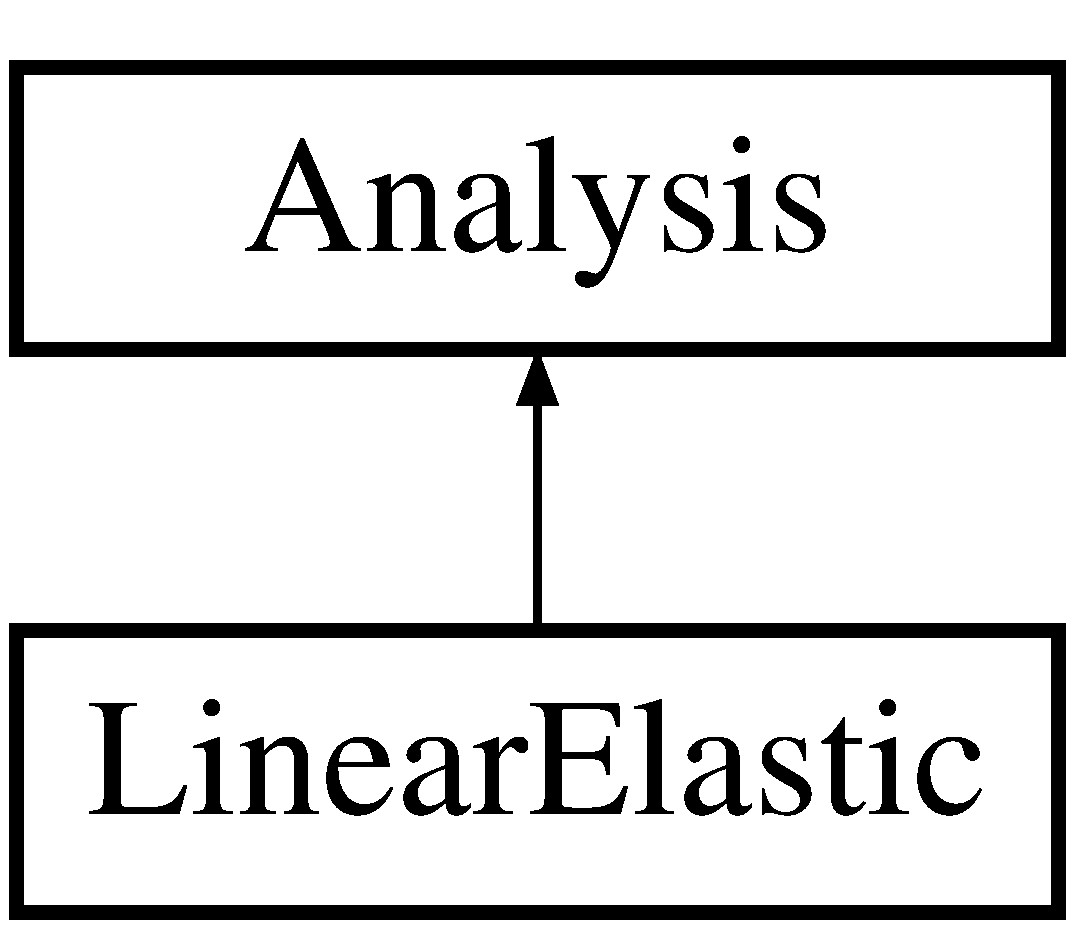
\includegraphics[height=2.000000cm]{class_analysis}
\end{center}
\end{figure}
\subsection*{Public Member Functions}
\begin{DoxyCompactItemize}
\item 
\mbox{\Hypertarget{class_analysis_a1cf251eb8dc62b30815ab5548ad88f73}\label{class_analysis_a1cf251eb8dc62b30815ab5548ad88f73}} 
\mbox{\hyperlink{class_analysis_a1cf251eb8dc62b30815ab5548ad88f73}{Analysis}} ()
\begin{DoxyCompactList}\small\item\em Default constructor for \mbox{\hyperlink{class_analysis}{Analysis}}. \end{DoxyCompactList}\item 
\mbox{\hyperlink{class_analysis_aae14526bb70c6372fd662b46aab74d2d}{Analysis}} (std\+::string const \&file\+Name)
\begin{DoxyCompactList}\small\item\em Custom constructor to create the mesh from input file for analysis. \end{DoxyCompactList}\item 
\mbox{\Hypertarget{class_analysis_a172ae0a3cbb68daa373baf081f5c00d9}\label{class_analysis_a172ae0a3cbb68daa373baf081f5c00d9}} 
virtual \mbox{\hyperlink{class_analysis_a172ae0a3cbb68daa373baf081f5c00d9}{$\sim$\+Analysis}} ()
\begin{DoxyCompactList}\small\item\em Virtual destructor for abstract class. \end{DoxyCompactList}\item 
\mbox{\Hypertarget{class_analysis_a951d32f9e28ea1a5942020f1304208ee}\label{class_analysis_a951d32f9e28ea1a5942020f1304208ee}} 
void \mbox{\hyperlink{class_analysis_a951d32f9e28ea1a5942020f1304208ee}{assemble\+Stiffness}} ()
\begin{DoxyCompactList}\small\item\em Assemble the global stiffness matrix from the local stiffness matrix of each element. \end{DoxyCompactList}\item 
\mbox{\Hypertarget{class_analysis_ab1c7b59927d7787ef75b0bba651b045c}\label{class_analysis_ab1c7b59927d7787ef75b0bba651b045c}} 
void \mbox{\hyperlink{class_analysis_ab1c7b59927d7787ef75b0bba651b045c}{apply\+Force}} ()
\begin{DoxyCompactList}\small\item\em Apply the load at nodes. \end{DoxyCompactList}\item 
\mbox{\Hypertarget{class_analysis_aec157316b08568c84d8d8344a724ff89}\label{class_analysis_aec157316b08568c84d8d8344a724ff89}} 
void \mbox{\hyperlink{class_analysis_aec157316b08568c84d8d8344a724ff89}{boundary\+Condition}} ()
\begin{DoxyCompactList}\small\item\em Designate boundary condition at nodes. \end{DoxyCompactList}\item 
\mbox{\Hypertarget{class_analysis_a93e6427625d7441986e8045da772892f}\label{class_analysis_a93e6427625d7441986e8045da772892f}} 
virtual void \mbox{\hyperlink{class_analysis_a93e6427625d7441986e8045da772892f}{solve\+Disp}} ()=0
\begin{DoxyCompactList}\small\item\em Solve for nodal displacement using different approaches. \end{DoxyCompactList}\item 
\mbox{\Hypertarget{class_analysis_a00c4b54646392d48ea2862ab3987a96d}\label{class_analysis_a00c4b54646392d48ea2862ab3987a96d}} 
void \mbox{\hyperlink{class_analysis_a00c4b54646392d48ea2862ab3987a96d}{compute\+Strain\+And\+Stress}} ()
\begin{DoxyCompactList}\small\item\em Compute nodal strain and stress from the extrapolation of results at Gaussian integration points and average the value over the mesh. \end{DoxyCompactList}\item 
\mbox{\Hypertarget{class_analysis_a6def63bf2890a4d9fa76c1af350703b8}\label{class_analysis_a6def63bf2890a4d9fa76c1af350703b8}} 
void \mbox{\hyperlink{class_analysis_a6def63bf2890a4d9fa76c1af350703b8}{print\+Disp}} () const
\begin{DoxyCompactList}\small\item\em Print the nodal displacement. \end{DoxyCompactList}\item 
\mbox{\Hypertarget{class_analysis_add0ccc185311df2140b66590b036b9fb}\label{class_analysis_add0ccc185311df2140b66590b036b9fb}} 
void \mbox{\hyperlink{class_analysis_add0ccc185311df2140b66590b036b9fb}{print\+Force}} () const
\begin{DoxyCompactList}\small\item\em Print the nodal force. \end{DoxyCompactList}\item 
\mbox{\Hypertarget{class_analysis_ab3087cac038045cc9cc4b8b8e200d16b}\label{class_analysis_ab3087cac038045cc9cc4b8b8e200d16b}} 
void \mbox{\hyperlink{class_analysis_ab3087cac038045cc9cc4b8b8e200d16b}{print\+Strain}} () const
\begin{DoxyCompactList}\small\item\em Print the nodal strain. \end{DoxyCompactList}\item 
\mbox{\Hypertarget{class_analysis_a81a4488de8e18d1c067c94a9edd2ac61}\label{class_analysis_a81a4488de8e18d1c067c94a9edd2ac61}} 
void \mbox{\hyperlink{class_analysis_a81a4488de8e18d1c067c94a9edd2ac61}{print\+Stress}} () const
\begin{DoxyCompactList}\small\item\em Print the nodal stress. \end{DoxyCompactList}\item 
\mbox{\Hypertarget{class_analysis_a0c17471cdbed978e4c4d62718e7b1578}\label{class_analysis_a0c17471cdbed978e4c4d62718e7b1578}} 
void \mbox{\hyperlink{class_analysis_a0c17471cdbed978e4c4d62718e7b1578}{write\+To\+File}} (std\+::string const \&file\+Name) const
\begin{DoxyCompactList}\small\item\em Write the outputs to file. \end{DoxyCompactList}\end{DoxyCompactItemize}
\subsection*{Protected Attributes}
\begin{DoxyCompactItemize}
\item 
\mbox{\Hypertarget{class_analysis_a34604f343af1a7d0ee2d19f2a905773b}\label{class_analysis_a34604f343af1a7d0ee2d19f2a905773b}} 
\mbox{\hyperlink{class_mesh}{Mesh}} \mbox{\hyperlink{class_analysis_a34604f343af1a7d0ee2d19f2a905773b}{mesh}}
\begin{DoxyCompactList}\small\item\em The mesh information of the problem. \end{DoxyCompactList}\item 
\mbox{\Hypertarget{class_analysis_a87256ae6f2ee1d1218b99bf287335fde}\label{class_analysis_a87256ae6f2ee1d1218b99bf287335fde}} 
Sparse\+Matrix$<$ double $>$ \mbox{\hyperlink{class_analysis_a87256ae6f2ee1d1218b99bf287335fde}{global\+Stiffness}}
\begin{DoxyCompactList}\small\item\em The global stiffness matrix as a 2n-\/by-\/2n sparse matrix. \end{DoxyCompactList}\item 
\mbox{\Hypertarget{class_analysis_a3e2cbd72b96f13d00c8758631c1d6bc9}\label{class_analysis_a3e2cbd72b96f13d00c8758631c1d6bc9}} 
Vector\+Xd \mbox{\hyperlink{class_analysis_a3e2cbd72b96f13d00c8758631c1d6bc9}{nodal\+Disp}}
\begin{DoxyCompactList}\small\item\em The nodal displacement 2n-\/by-\/1 vector. \end{DoxyCompactList}\item 
\mbox{\Hypertarget{class_analysis_aab2110fe7a0fffd9dd738ed9c5f45012}\label{class_analysis_aab2110fe7a0fffd9dd738ed9c5f45012}} 
Vector\+Xd \mbox{\hyperlink{class_analysis_aab2110fe7a0fffd9dd738ed9c5f45012}{nodal\+Force}}
\begin{DoxyCompactList}\small\item\em The nodal force 2n-\/by-\/1 vector. \end{DoxyCompactList}\item 
\mbox{\Hypertarget{class_analysis_a9fa4ad52de8cc42341212d09622949c7}\label{class_analysis_a9fa4ad52de8cc42341212d09622949c7}} 
Matrix\+Xd \mbox{\hyperlink{class_analysis_a9fa4ad52de8cc42341212d09622949c7}{nodal\+Strain}}
\begin{DoxyCompactList}\small\item\em The nodal strain n-\/by-\/4 matrix. \end{DoxyCompactList}\item 
\mbox{\Hypertarget{class_analysis_ae0e69d62aa3cd400b1ae46f430a59cb3}\label{class_analysis_ae0e69d62aa3cd400b1ae46f430a59cb3}} 
Matrix\+Xd \mbox{\hyperlink{class_analysis_ae0e69d62aa3cd400b1ae46f430a59cb3}{nodal\+Stress}}
\begin{DoxyCompactList}\small\item\em The nodal strain n-\/by-\/4 matrix. \end{DoxyCompactList}\end{DoxyCompactItemize}


\subsection{Detailed Description}


Definition at line 41 of file Analysis.\+h.



\subsection{Constructor \& Destructor Documentation}
\mbox{\Hypertarget{class_analysis_aae14526bb70c6372fd662b46aab74d2d}\label{class_analysis_aae14526bb70c6372fd662b46aab74d2d}} 
\index{Analysis@{Analysis}!Analysis@{Analysis}}
\index{Analysis@{Analysis}!Analysis@{Analysis}}
\subsubsection{\texorpdfstring{Analysis()}{Analysis()}}
{\footnotesize\ttfamily Analysis\+::\+Analysis (\begin{DoxyParamCaption}\item[{std\+::string const \&}]{file\+Name }\end{DoxyParamCaption})}



Custom constructor to create the mesh from input file for analysis. 


\begin{DoxyParams}{Parameters}
{\em file\+Name} & The path to the input file. \\
\hline
\end{DoxyParams}


Definition at line 18 of file Analysis.\+cpp.



The documentation for this class was generated from the following files\+:\begin{DoxyCompactItemize}
\item 
\mbox{\hyperlink{_analysis_8h}{Analysis.\+h}}\item 
\mbox{\hyperlink{_analysis_8cpp}{Analysis.\+cpp}}\end{DoxyCompactItemize}

\hypertarget{class_element}{}\section{Element Class Reference}
\label{class_element}\index{Element@{Element}}
Inheritance diagram for Element\+:\begin{figure}[H]
\begin{center}
\leavevmode
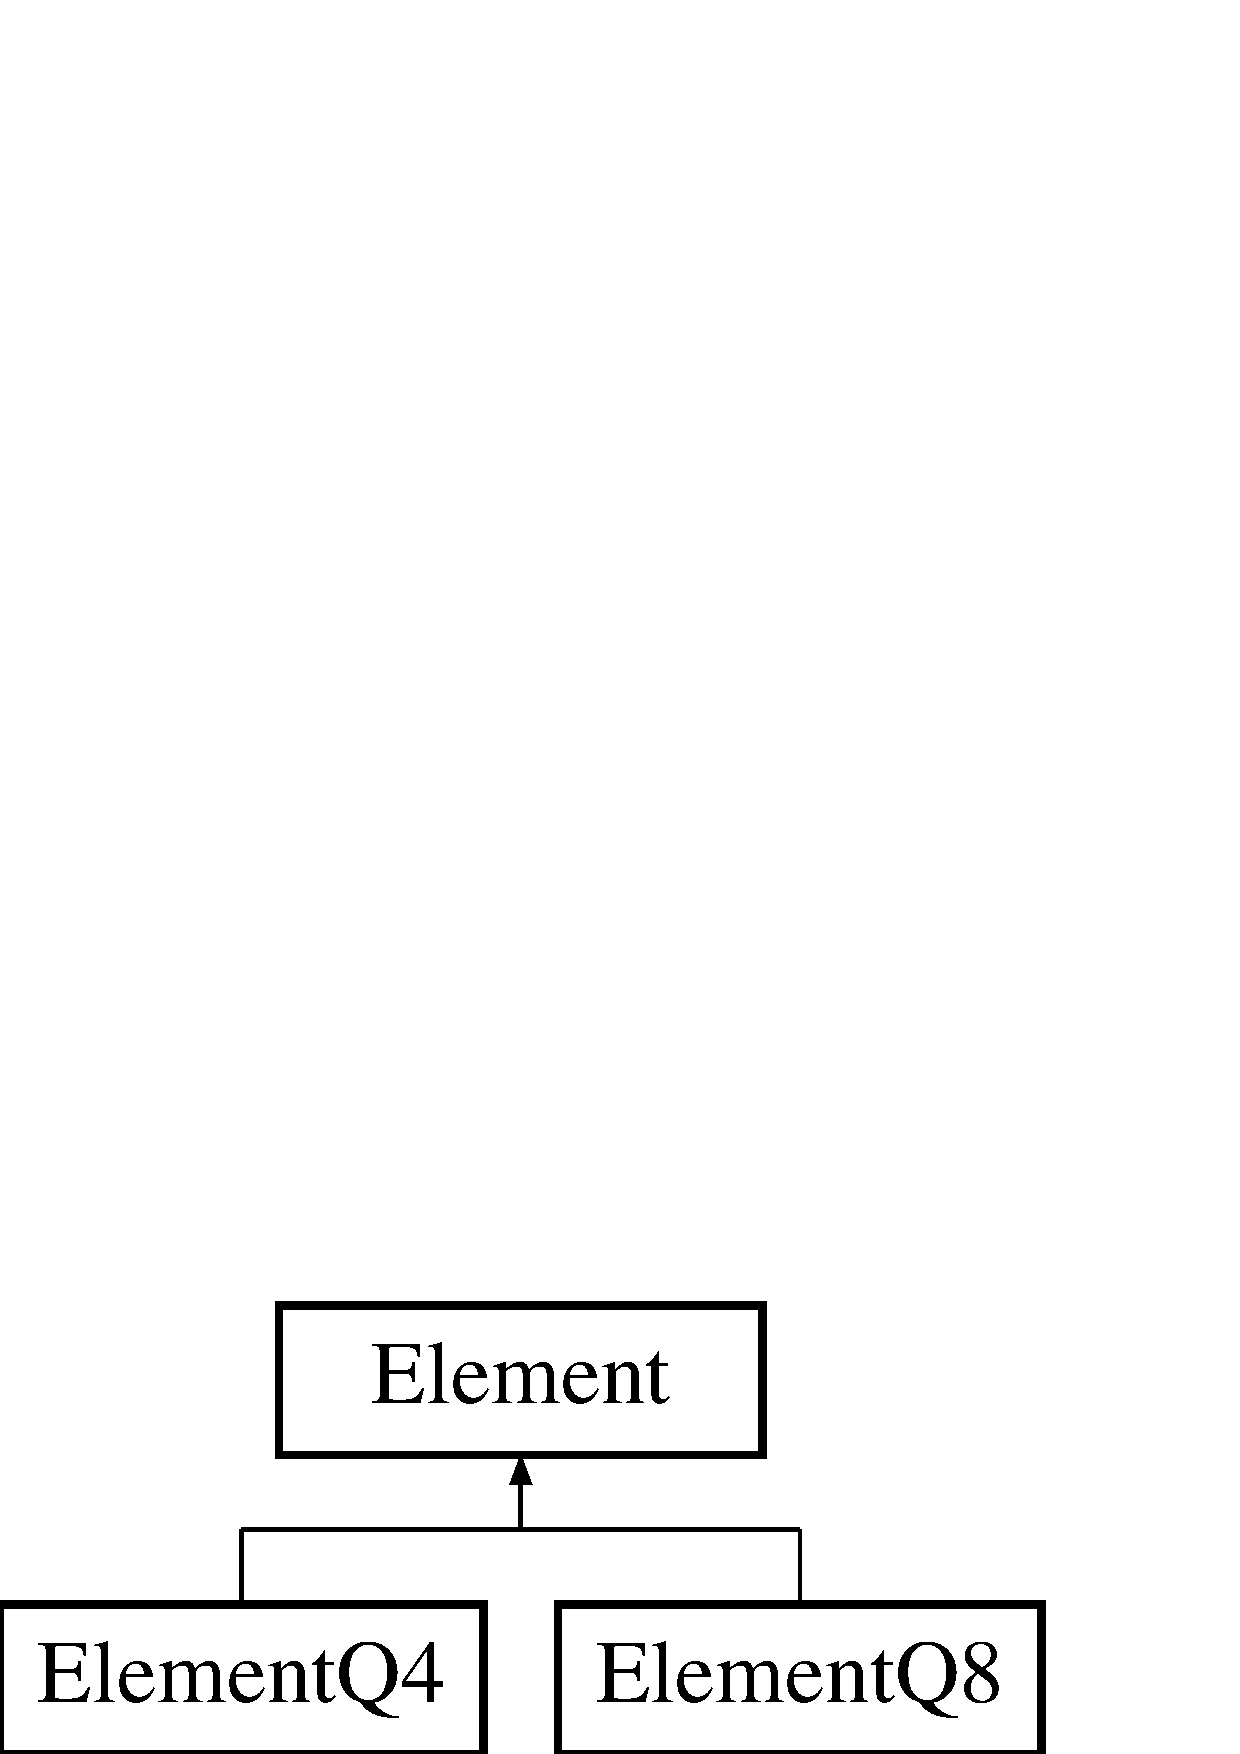
\includegraphics[height=2.000000cm]{class_element}
\end{center}
\end{figure}
\subsection*{Public Member Functions}
\begin{DoxyCompactItemize}
\item 
\mbox{\Hypertarget{class_element_ab0d0e20be9a36ae676202db753faeec9}\label{class_element_ab0d0e20be9a36ae676202db753faeec9}} 
\mbox{\hyperlink{class_element_ab0d0e20be9a36ae676202db753faeec9}{Element}} ()
\begin{DoxyCompactList}\small\item\em Default constructor for \mbox{\hyperlink{class_element}{Element}}. \end{DoxyCompactList}\item 
\mbox{\hyperlink{class_element_a05c744ed2de597b38da74c7765f5ed1b}{Element}} (const int \&index, const std\+::vector$<$ int $>$ \&node\+List, \mbox{\hyperlink{class_node}{Node}} $\ast$$\ast$const mesh\+Node)
\begin{DoxyCompactList}\small\item\em Custom constructor to create an element with given node indices. \end{DoxyCompactList}\item 
\mbox{\Hypertarget{class_element_a68700ab3d0e5551cb456e91c3a8fc61b}\label{class_element_a68700ab3d0e5551cb456e91c3a8fc61b}} 
\mbox{\hyperlink{class_element_a68700ab3d0e5551cb456e91c3a8fc61b}{Element}} (\mbox{\hyperlink{class_element}{Element}} const \&other)
\begin{DoxyCompactList}\small\item\em Copy constructor. \end{DoxyCompactList}\item 
\mbox{\Hypertarget{class_element_a2baffaa8af3b584a906206d0381cd204}\label{class_element_a2baffaa8af3b584a906206d0381cd204}} 
\mbox{\hyperlink{class_element}{Element}} const  \& \mbox{\hyperlink{class_element_a2baffaa8af3b584a906206d0381cd204}{operator=}} (\mbox{\hyperlink{class_element}{Element}} const \&other)
\begin{DoxyCompactList}\small\item\em Assignment operator. \end{DoxyCompactList}\item 
virtual \mbox{\hyperlink{class_element_a13d54ba9c08b6bec651402f1c2bb002c}{$\sim$\+Element}} ()
\begin{DoxyCompactList}\small\item\em Destructor. \end{DoxyCompactList}\item 
void \mbox{\hyperlink{class_element_ad74b47354fe0608c9baba38c79e5b549}{set\+Material}} (const double \&M, const double \&v)
\begin{DoxyCompactList}\small\item\em Assign the material properties of the element. \end{DoxyCompactList}\item 
const Matrix\+Xd \& \mbox{\hyperlink{class_element_abd9d11d211f4f5e6f9e213a1013f36ed}{E\+Matrix}} () const
\begin{DoxyCompactList}\small\item\em Get the stress-\/strain constitutive matrix of the element. \end{DoxyCompactList}\item 
virtual const Matrix\+Xd \& \mbox{\hyperlink{class_element_a603fbe060b5d6979506f0d2130e6c171}{local\+Stiffness}} ()=0
\begin{DoxyCompactList}\small\item\em Compute the local element stiffness matrix formulated by differentiation of element strain energy and numerical integration (Gaussian quadrature). \end{DoxyCompactList}\item 
virtual Matrix\+Xd \mbox{\hyperlink{class_element_ad469c745f0bcb9d7a3431b1608c1ade6}{jacobian}} (const Vector2d \&point) const =0
\begin{DoxyCompactList}\small\item\em Compute the Jacobian coordinates transformation matrix at a given point. \end{DoxyCompactList}\item 
virtual Matrix\+Xd \mbox{\hyperlink{class_element_ae3c88315d1a30addff6379a9089465ca}{B\+Matrix}} (const Vector2d \&gaussian\+Point) const =0
\begin{DoxyCompactList}\small\item\em Compute the strain-\/displacement constitutive matrix. \end{DoxyCompactList}\item 
virtual \mbox{\hyperlink{class_shape}{Shape}} $\ast$const \mbox{\hyperlink{class_element_a54c5c297abff4ac3abacd815342a9645}{get\+Shape}} () const =0
\begin{DoxyCompactList}\small\item\em Get the shape object of this element. \end{DoxyCompactList}\item 
const int \& \mbox{\hyperlink{class_element_a85dc312253f1d39c29659393fbb1d485}{get\+Index}} () const
\begin{DoxyCompactList}\small\item\em Get the index of this element. \end{DoxyCompactList}\item 
const int \& \mbox{\hyperlink{class_element_a0221b246d9ca632136cc39790c46ee8f}{get\+Size}} () const
\begin{DoxyCompactList}\small\item\em Get the size/type of this element. \end{DoxyCompactList}\item 
const Vector\+Xi \& \mbox{\hyperlink{class_element_a763e0e4a46e68823903557a605dc5474}{get\+Node\+List}} () const
\begin{DoxyCompactList}\small\item\em Get the list of nodes belong to this element. \end{DoxyCompactList}\item 
const Matrix\+Xd \& \mbox{\hyperlink{class_element_a4d12b24e62592a1456e04d15872d5240}{get\+Node\+Coord}} () const
\begin{DoxyCompactList}\small\item\em Get the stacked coordinates matrix of the nodes belong to this element. \end{DoxyCompactList}\end{DoxyCompactItemize}
\subsection*{Public Attributes}
\begin{DoxyCompactItemize}
\item 
\mbox{\Hypertarget{class_element_adb81184f683d1eebb5b3a28887ff8df4}\label{class_element_adb81184f683d1eebb5b3a28887ff8df4}} 
Matrix\+Xd \mbox{\hyperlink{class_element_adb81184f683d1eebb5b3a28887ff8df4}{local\+Stiff}}
\begin{DoxyCompactList}\small\item\em The 2n-\/by-\/2n local stiffness matrix where n is the number of nodes. \end{DoxyCompactList}\end{DoxyCompactItemize}


\subsection{Detailed Description}


Definition at line 23 of file Element.\+h.



\subsection{Constructor \& Destructor Documentation}
\mbox{\Hypertarget{class_element_a05c744ed2de597b38da74c7765f5ed1b}\label{class_element_a05c744ed2de597b38da74c7765f5ed1b}} 
\index{Element@{Element}!Element@{Element}}
\index{Element@{Element}!Element@{Element}}
\subsubsection{\texorpdfstring{Element()}{Element()}}
{\footnotesize\ttfamily Element\+::\+Element (\begin{DoxyParamCaption}\item[{const int \&}]{index,  }\item[{const std\+::vector$<$ int $>$ \&}]{node\+List,  }\item[{\mbox{\hyperlink{class_node}{Node}} $\ast$$\ast$const}]{mesh\+Node }\end{DoxyParamCaption})}



Custom constructor to create an element with given node indices. 


\begin{DoxyParams}{Parameters}
{\em index} & The index number of current element. \\
\hline
{\em node\+List} & The list of node indices this element is consist of. \\
\hline
{\em mesh\+Node} & \mbox{\hyperlink{class_a}{A}} const pointer to the node pool of the mesh.\\
\hline
\end{DoxyParams}
\begin{DoxyNote}{Note}
Old version of this function pass in all the nodes, which is expensive. This optimized version only pass in a pointer to access the node pool of the mesh. 
\end{DoxyNote}


Definition at line 16 of file Element.\+cpp.

\mbox{\Hypertarget{class_element_a13d54ba9c08b6bec651402f1c2bb002c}\label{class_element_a13d54ba9c08b6bec651402f1c2bb002c}} 
\index{Element@{Element}!````~Element@{$\sim$\+Element}}
\index{````~Element@{$\sim$\+Element}!Element@{Element}}
\subsubsection{\texorpdfstring{$\sim$\+Element()}{~Element()}}
{\footnotesize\ttfamily Element\+::$\sim$\+Element (\begin{DoxyParamCaption}{ }\end{DoxyParamCaption})\hspace{0.3cm}{\ttfamily [virtual]}}



Destructor. 

\begin{DoxyNote}{Note}
As an abstract class, the destructor must be virtual. 
\end{DoxyNote}


Definition at line 41 of file Element.\+cpp.



\subsection{Member Function Documentation}
\mbox{\Hypertarget{class_element_ae3c88315d1a30addff6379a9089465ca}\label{class_element_ae3c88315d1a30addff6379a9089465ca}} 
\index{Element@{Element}!B\+Matrix@{B\+Matrix}}
\index{B\+Matrix@{B\+Matrix}!Element@{Element}}
\subsubsection{\texorpdfstring{B\+Matrix()}{BMatrix()}}
{\footnotesize\ttfamily virtual Matrix\+Xd Element\+::\+B\+Matrix (\begin{DoxyParamCaption}\item[{const Vector2d \&}]{gaussian\+Point }\end{DoxyParamCaption}) const\hspace{0.3cm}{\ttfamily [pure virtual]}}



Compute the strain-\/displacement constitutive matrix. 

e = D$\ast$u = D$\ast$(N$\ast$u) = (D$\ast$N)u = Bu, so \mbox{\hyperlink{class_b}{B}} is the differential matrix multiplying the shape function.


\begin{DoxyParams}{Parameters}
{\em gaussian\+Point} & The Gaussian point where the \mbox{\hyperlink{class_b}{B}} matrix to be evaluated. \\
\hline
\end{DoxyParams}
\begin{DoxyReturn}{Returns}
The 4-\/by-\/2n \mbox{\hyperlink{class_b}{B}} matrix where n is the number of nodes belong to this element. 
\end{DoxyReturn}


Implemented in \mbox{\hyperlink{class_element_q8_afb41facf96d5bb4be5162724699e3e02}{Element\+Q8}}, and \mbox{\hyperlink{class_element_q4_a092a9584a1b3b22cd929246ba100f91a}{Element\+Q4}}.

\mbox{\Hypertarget{class_element_abd9d11d211f4f5e6f9e213a1013f36ed}\label{class_element_abd9d11d211f4f5e6f9e213a1013f36ed}} 
\index{Element@{Element}!E\+Matrix@{E\+Matrix}}
\index{E\+Matrix@{E\+Matrix}!Element@{Element}}
\subsubsection{\texorpdfstring{E\+Matrix()}{EMatrix()}}
{\footnotesize\ttfamily const Matrix\+Xd \& Element\+::\+E\+Matrix (\begin{DoxyParamCaption}{ }\end{DoxyParamCaption}) const}



Get the stress-\/strain constitutive matrix of the element. 

\begin{DoxyReturn}{Returns}
The 4-\/by-\/4 E matrix. 
\end{DoxyReturn}


Definition at line 59 of file Element.\+cpp.

\mbox{\Hypertarget{class_element_a85dc312253f1d39c29659393fbb1d485}\label{class_element_a85dc312253f1d39c29659393fbb1d485}} 
\index{Element@{Element}!get\+Index@{get\+Index}}
\index{get\+Index@{get\+Index}!Element@{Element}}
\subsubsection{\texorpdfstring{get\+Index()}{getIndex()}}
{\footnotesize\ttfamily const int \& Element\+::get\+Index (\begin{DoxyParamCaption}{ }\end{DoxyParamCaption}) const}



Get the index of this element. 

\begin{DoxyReturn}{Returns}
The index. 
\end{DoxyReturn}


Definition at line 64 of file Element.\+cpp.

\mbox{\Hypertarget{class_element_a4d12b24e62592a1456e04d15872d5240}\label{class_element_a4d12b24e62592a1456e04d15872d5240}} 
\index{Element@{Element}!get\+Node\+Coord@{get\+Node\+Coord}}
\index{get\+Node\+Coord@{get\+Node\+Coord}!Element@{Element}}
\subsubsection{\texorpdfstring{get\+Node\+Coord()}{getNodeCoord()}}
{\footnotesize\ttfamily const Matrix\+Xd \& Element\+::get\+Node\+Coord (\begin{DoxyParamCaption}{ }\end{DoxyParamCaption}) const}



Get the stacked coordinates matrix of the nodes belong to this element. 

\begin{DoxyReturn}{Returns}
The node coordinates as a n-\/by-\/2 matrix. 
\end{DoxyReturn}


Definition at line 79 of file Element.\+cpp.

\mbox{\Hypertarget{class_element_a763e0e4a46e68823903557a605dc5474}\label{class_element_a763e0e4a46e68823903557a605dc5474}} 
\index{Element@{Element}!get\+Node\+List@{get\+Node\+List}}
\index{get\+Node\+List@{get\+Node\+List}!Element@{Element}}
\subsubsection{\texorpdfstring{get\+Node\+List()}{getNodeList()}}
{\footnotesize\ttfamily const Vector\+Xi \& Element\+::get\+Node\+List (\begin{DoxyParamCaption}{ }\end{DoxyParamCaption}) const}



Get the list of nodes belong to this element. 

\begin{DoxyReturn}{Returns}
The node list as a n-\/by-\/1 vector. 
\end{DoxyReturn}


Definition at line 74 of file Element.\+cpp.

\mbox{\Hypertarget{class_element_a54c5c297abff4ac3abacd815342a9645}\label{class_element_a54c5c297abff4ac3abacd815342a9645}} 
\index{Element@{Element}!get\+Shape@{get\+Shape}}
\index{get\+Shape@{get\+Shape}!Element@{Element}}
\subsubsection{\texorpdfstring{get\+Shape()}{getShape()}}
{\footnotesize\ttfamily virtual \mbox{\hyperlink{class_shape}{Shape}}$\ast$ const Element\+::get\+Shape (\begin{DoxyParamCaption}{ }\end{DoxyParamCaption}) const\hspace{0.3cm}{\ttfamily [pure virtual]}}



Get the shape object of this element. 

\begin{DoxyReturn}{Returns}
\mbox{\hyperlink{class_a}{A}} pointer to the shape object of this element.
\end{DoxyReturn}
\begin{DoxyNote}{Note}
For different element, we would have different shape property, so we return a generic polymorphed \mbox{\hyperlink{class_shape}{Shape}} class pointer to achieve the standardized behavior of our program. It should also be noted that this is a virtual method, and the \mbox{\hyperlink{class_shape}{Shape}} property of each element type is stored as a static member of that class. This is really an elegant solution to pave our path towards the hybrid element case. And returning a const pointer secures the usage of shape object. 
\end{DoxyNote}


Implemented in \mbox{\hyperlink{class_element_q8_a06118e8d0c0a0cb247c249f22e11eeaf}{Element\+Q8}}, and \mbox{\hyperlink{class_element_q4_a3e2b762e838f20a10c184f55d3d4ff85}{Element\+Q4}}.

\mbox{\Hypertarget{class_element_a0221b246d9ca632136cc39790c46ee8f}\label{class_element_a0221b246d9ca632136cc39790c46ee8f}} 
\index{Element@{Element}!get\+Size@{get\+Size}}
\index{get\+Size@{get\+Size}!Element@{Element}}
\subsubsection{\texorpdfstring{get\+Size()}{getSize()}}
{\footnotesize\ttfamily const int \& Element\+::get\+Size (\begin{DoxyParamCaption}{ }\end{DoxyParamCaption}) const}



Get the size/type of this element. 

\begin{DoxyReturn}{Returns}
The size/type. 
\end{DoxyReturn}


Definition at line 69 of file Element.\+cpp.

\mbox{\Hypertarget{class_element_ad469c745f0bcb9d7a3431b1608c1ade6}\label{class_element_ad469c745f0bcb9d7a3431b1608c1ade6}} 
\index{Element@{Element}!jacobian@{jacobian}}
\index{jacobian@{jacobian}!Element@{Element}}
\subsubsection{\texorpdfstring{jacobian()}{jacobian()}}
{\footnotesize\ttfamily virtual Matrix\+Xd Element\+::jacobian (\begin{DoxyParamCaption}\item[{const Vector2d \&}]{point }\end{DoxyParamCaption}) const\hspace{0.3cm}{\ttfamily [pure virtual]}}



Compute the Jacobian coordinates transformation matrix at a given point. 


\begin{DoxyParams}{Parameters}
{\em point} & The point where the Jacobian matrix to be evaluated. \\
\hline
\end{DoxyParams}
\begin{DoxyReturn}{Returns}
The 2-\/by-\/2 (2D) Jacobian matrix. 
\end{DoxyReturn}


Implemented in \mbox{\hyperlink{class_element_q8_ae23bf98a466daa224224da495d5724ff}{Element\+Q8}}, and \mbox{\hyperlink{class_element_q4_a1347c3ce4ef1c34a16aa72fdf593932d}{Element\+Q4}}.

\mbox{\Hypertarget{class_element_a603fbe060b5d6979506f0d2130e6c171}\label{class_element_a603fbe060b5d6979506f0d2130e6c171}} 
\index{Element@{Element}!local\+Stiffness@{local\+Stiffness}}
\index{local\+Stiffness@{local\+Stiffness}!Element@{Element}}
\subsubsection{\texorpdfstring{local\+Stiffness()}{localStiffness()}}
{\footnotesize\ttfamily virtual const Matrix\+Xd\& Element\+::local\+Stiffness (\begin{DoxyParamCaption}{ }\end{DoxyParamCaption})\hspace{0.3cm}{\ttfamily [pure virtual]}}



Compute the local element stiffness matrix formulated by differentiation of element strain energy and numerical integration (Gaussian quadrature). 

\begin{DoxyReturn}{Returns}
The 2n-\/by-\/2n element stiffness matrix where n is number of nodes belong to this element. 
\end{DoxyReturn}


Implemented in \mbox{\hyperlink{class_element_q8_afc898e404f9abb5a5a4d74eee54476b7}{Element\+Q8}}, and \mbox{\hyperlink{class_element_q4_a9a127fdfd6f80efe3c35f20d7b1296cf}{Element\+Q4}}.

\mbox{\Hypertarget{class_element_ad74b47354fe0608c9baba38c79e5b549}\label{class_element_ad74b47354fe0608c9baba38c79e5b549}} 
\index{Element@{Element}!set\+Material@{set\+Material}}
\index{set\+Material@{set\+Material}!Element@{Element}}
\subsubsection{\texorpdfstring{set\+Material()}{setMaterial()}}
{\footnotesize\ttfamily void Element\+::set\+Material (\begin{DoxyParamCaption}\item[{const double \&}]{M,  }\item[{const double \&}]{v }\end{DoxyParamCaption})}



Assign the material properties of the element. 


\begin{DoxyParams}{Parameters}
{\em M} & The modulus. \\
\hline
{\em v} & The Poisson\textquotesingle{}s ratio. \\
\hline
\end{DoxyParams}


Definition at line 46 of file Element.\+cpp.



The documentation for this class was generated from the following files\+:\begin{DoxyCompactItemize}
\item 
\mbox{\hyperlink{_element_8h}{Element.\+h}}\item 
\mbox{\hyperlink{_element_8cpp}{Element.\+cpp}}\end{DoxyCompactItemize}

\hypertarget{class_element_q4}{}\section{Element\+Q4 Class Reference}
\label{class_element_q4}\index{Element\+Q4@{Element\+Q4}}
Inheritance diagram for Element\+Q4\+:\begin{figure}[H]
\begin{center}
\leavevmode
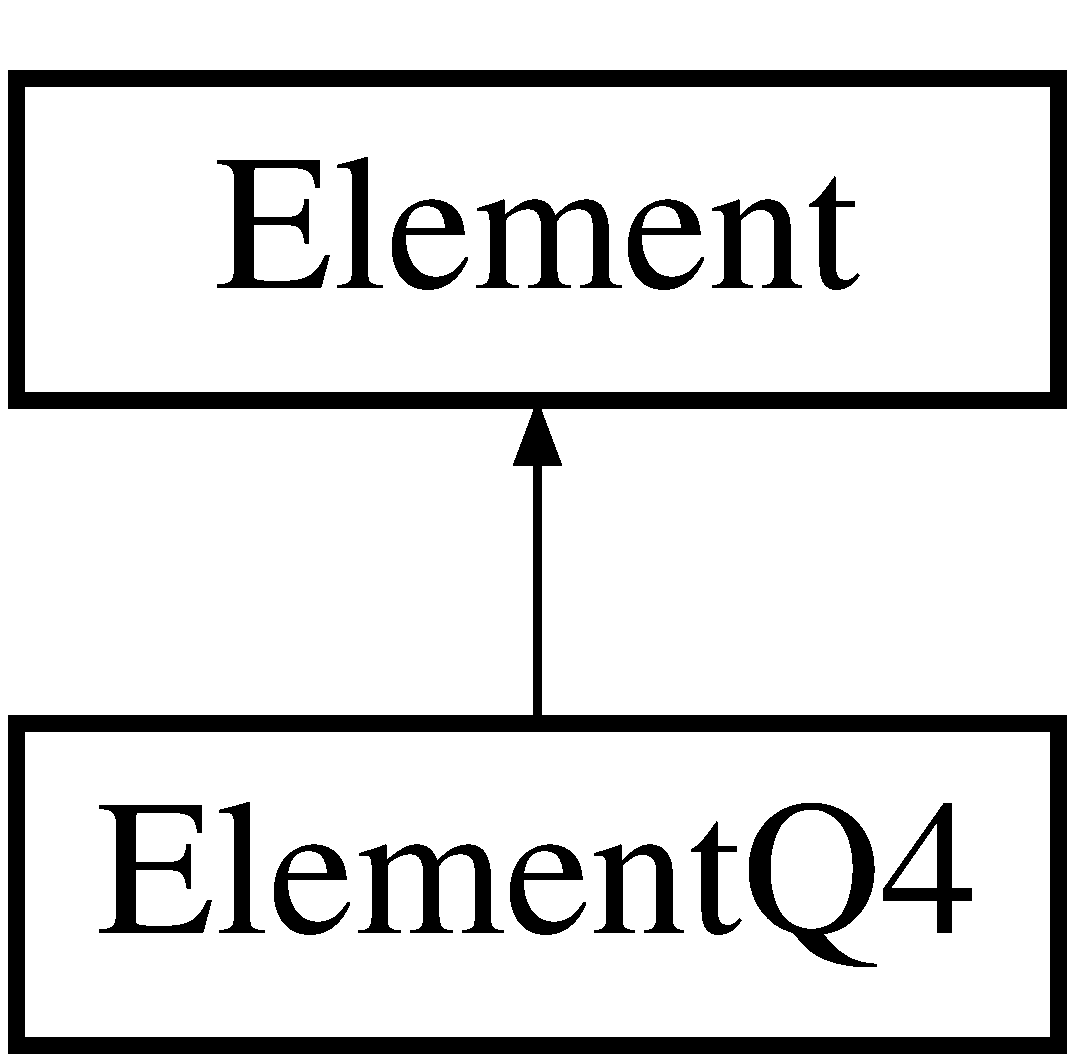
\includegraphics[height=2.000000cm]{class_element_q4}
\end{center}
\end{figure}
\subsection*{Public Member Functions}
\begin{DoxyCompactItemize}
\item 
\mbox{\Hypertarget{class_element_q4_ab119a15023a7abb356d5db5961e2febb}\label{class_element_q4_ab119a15023a7abb356d5db5961e2febb}} 
{\bfseries Element\+Q4} (const int \&index, const std\+::vector$<$ int $>$ \&node\+List, \mbox{\hyperlink{class_node}{Node}} $\ast$$\ast$const mesh\+Node)
\item 
const Matrix\+Xd \& \mbox{\hyperlink{class_element_q4_a9a127fdfd6f80efe3c35f20d7b1296cf}{local\+Stiffness}} ()
\begin{DoxyCompactList}\small\item\em Compute the local element stiffness matrix formulated by differentiation of element strain energy and numerical integration (Gaussian quadrature). \end{DoxyCompactList}\item 
Matrix\+Xd \mbox{\hyperlink{class_element_q4_a1347c3ce4ef1c34a16aa72fdf593932d}{jacobian}} (const Vector2d \&point) const
\begin{DoxyCompactList}\small\item\em Compute the Jacobian coordinates transformation matrix at a given point. \end{DoxyCompactList}\item 
Matrix\+Xd \mbox{\hyperlink{class_element_q4_a092a9584a1b3b22cd929246ba100f91a}{B\+Matrix}} (const Vector2d \&gaussian\+Point) const
\begin{DoxyCompactList}\small\item\em Compute the strain-\/displacement constitutive matrix. \end{DoxyCompactList}\item 
\mbox{\hyperlink{class_shape}{Shape}} $\ast$const \mbox{\hyperlink{class_element_q4_a3e2b762e838f20a10c184f55d3d4ff85}{get\+Shape}} () const
\begin{DoxyCompactList}\small\item\em Get the shape object of this element. \end{DoxyCompactList}\end{DoxyCompactItemize}
\subsection*{Additional Inherited Members}


\subsection{Member Function Documentation}
\mbox{\Hypertarget{class_element_q4_a092a9584a1b3b22cd929246ba100f91a}\label{class_element_q4_a092a9584a1b3b22cd929246ba100f91a}} 
\index{Element\+Q4@{Element\+Q4}!B\+Matrix@{B\+Matrix}}
\index{B\+Matrix@{B\+Matrix}!Element\+Q4@{Element\+Q4}}
\subsubsection{\texorpdfstring{B\+Matrix()}{BMatrix()}}
{\footnotesize\ttfamily Matrix\+Xd Element\+Q4\+::\+B\+Matrix (\begin{DoxyParamCaption}\item[{const Vector2d \&}]{gaussian\+Point }\end{DoxyParamCaption}) const\hspace{0.3cm}{\ttfamily [virtual]}}



Compute the strain-\/displacement constitutive matrix. 

e = D$\ast$u = D$\ast$(N$\ast$u) = (D$\ast$N)u = Bu, so B is the differential matrix multiplying the shape function.


\begin{DoxyParams}{Parameters}
{\em gaussian\+Point} & The Gaussian point where the B matrix to be evaluated. \\
\hline
\end{DoxyParams}
\begin{DoxyReturn}{Returns}
The 4-\/by-\/2n B matrix where n is the number of nodes belong to this element. 
\end{DoxyReturn}


Implements \mbox{\hyperlink{class_element_ae3c88315d1a30addff6379a9089465ca}{Element}}.

\mbox{\Hypertarget{class_element_q4_a3e2b762e838f20a10c184f55d3d4ff85}\label{class_element_q4_a3e2b762e838f20a10c184f55d3d4ff85}} 
\index{Element\+Q4@{Element\+Q4}!get\+Shape@{get\+Shape}}
\index{get\+Shape@{get\+Shape}!Element\+Q4@{Element\+Q4}}
\subsubsection{\texorpdfstring{get\+Shape()}{getShape()}}
{\footnotesize\ttfamily \mbox{\hyperlink{class_shape}{Shape}} $\ast$const Element\+Q4\+::get\+Shape (\begin{DoxyParamCaption}{ }\end{DoxyParamCaption}) const\hspace{0.3cm}{\ttfamily [virtual]}}



Get the shape object of this element. 

\begin{DoxyReturn}{Returns}
A pointer to the shape object of this element.
\end{DoxyReturn}
\begin{DoxyNote}{Note}
For different element, we would have different shape property, so we return a generic polymorphed \mbox{\hyperlink{class_shape}{Shape}} class pointer to achieve the standardized behavior of our program. It should also be noted that this is a virtual method, and the \mbox{\hyperlink{class_shape}{Shape}} property of each element type is stored as a static member of that class. This is really an elegant solution to pave our path towards the hybrid element case. And returning a const pointer secures the usage of shape object. 
\end{DoxyNote}


Implements \mbox{\hyperlink{class_element_a54c5c297abff4ac3abacd815342a9645}{Element}}.

\mbox{\Hypertarget{class_element_q4_a1347c3ce4ef1c34a16aa72fdf593932d}\label{class_element_q4_a1347c3ce4ef1c34a16aa72fdf593932d}} 
\index{Element\+Q4@{Element\+Q4}!jacobian@{jacobian}}
\index{jacobian@{jacobian}!Element\+Q4@{Element\+Q4}}
\subsubsection{\texorpdfstring{jacobian()}{jacobian()}}
{\footnotesize\ttfamily Matrix\+Xd Element\+Q4\+::jacobian (\begin{DoxyParamCaption}\item[{const Vector2d \&}]{point }\end{DoxyParamCaption}) const\hspace{0.3cm}{\ttfamily [virtual]}}



Compute the Jacobian coordinates transformation matrix at a given point. 


\begin{DoxyParams}{Parameters}
{\em point} & The point where the Jacobian matrix to be evaluated. \\
\hline
\end{DoxyParams}
\begin{DoxyReturn}{Returns}
The 2-\/by-\/2 (2D) Jacobian matrix. 
\end{DoxyReturn}


Implements \mbox{\hyperlink{class_element_ad469c745f0bcb9d7a3431b1608c1ade6}{Element}}.

\mbox{\Hypertarget{class_element_q4_a9a127fdfd6f80efe3c35f20d7b1296cf}\label{class_element_q4_a9a127fdfd6f80efe3c35f20d7b1296cf}} 
\index{Element\+Q4@{Element\+Q4}!local\+Stiffness@{local\+Stiffness}}
\index{local\+Stiffness@{local\+Stiffness}!Element\+Q4@{Element\+Q4}}
\subsubsection{\texorpdfstring{local\+Stiffness()}{localStiffness()}}
{\footnotesize\ttfamily const Matrix\+Xd \& Element\+Q4\+::local\+Stiffness (\begin{DoxyParamCaption}{ }\end{DoxyParamCaption})\hspace{0.3cm}{\ttfamily [virtual]}}



Compute the local element stiffness matrix formulated by differentiation of element strain energy and numerical integration (Gaussian quadrature). 

\begin{DoxyReturn}{Returns}
The 2n-\/by-\/2n element stiffness matrix where n is number of nodes belong to this element. 
\end{DoxyReturn}


Implements \mbox{\hyperlink{class_element_a603fbe060b5d6979506f0d2130e6c171}{Element}}.



The documentation for this class was generated from the following files\+:\begin{DoxyCompactItemize}
\item 
\mbox{\hyperlink{_element_q4_8h}{Element\+Q4.\+h}}\item 
\mbox{\hyperlink{_element_q4_8cpp}{Element\+Q4.\+cpp}}\end{DoxyCompactItemize}

\hypertarget{class_element_q8}{}\section{Element\+Q8 Class Reference}
\label{class_element_q8}\index{Element\+Q8@{Element\+Q8}}
Inheritance diagram for Element\+Q8\+:\begin{figure}[H]
\begin{center}
\leavevmode
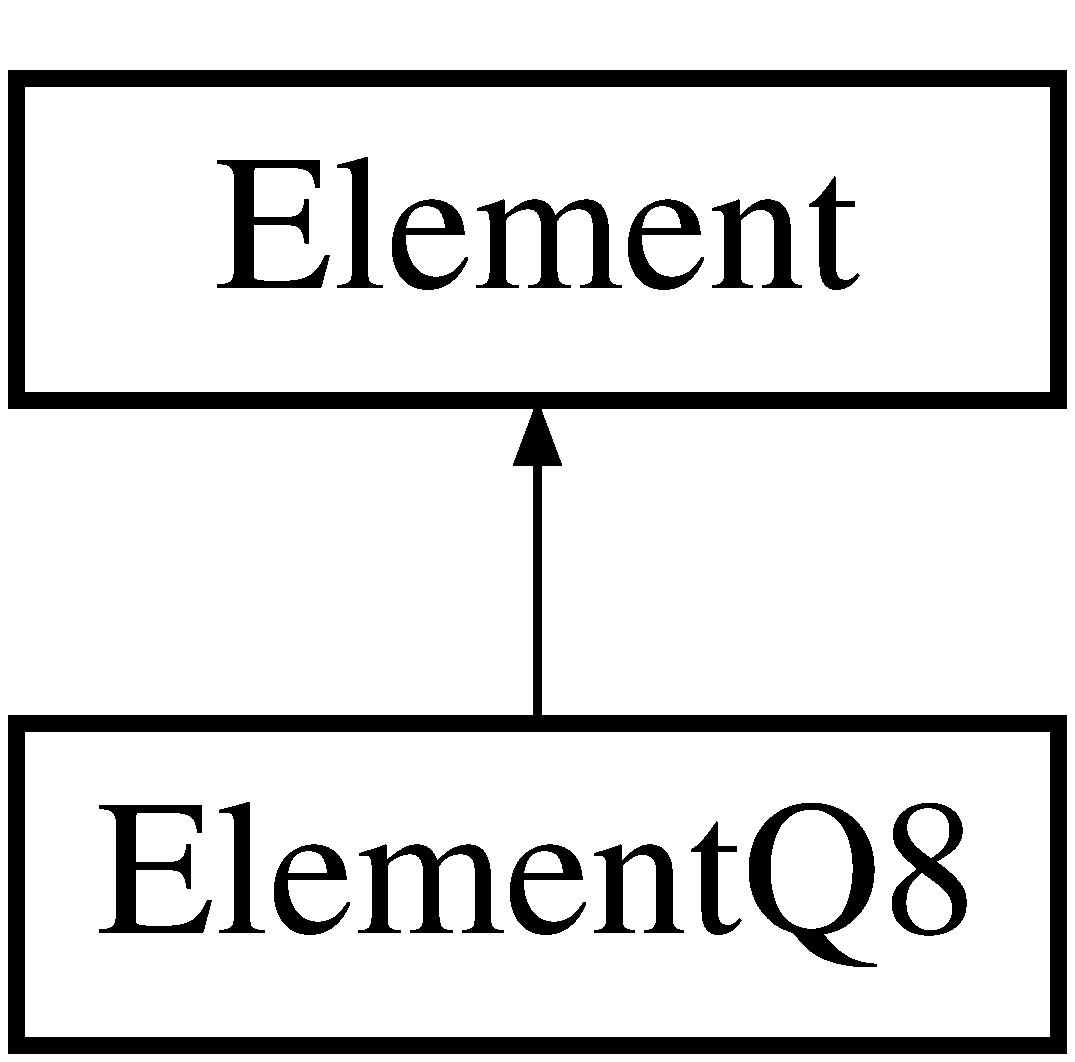
\includegraphics[height=2.000000cm]{class_element_q8}
\end{center}
\end{figure}
\subsection*{Public Member Functions}
\begin{DoxyCompactItemize}
\item 
\mbox{\Hypertarget{class_element_q8_a62c1f93cb438055e8412b3f957e72a20}\label{class_element_q8_a62c1f93cb438055e8412b3f957e72a20}} 
{\bfseries Element\+Q8} (const int \&index, const std\+::vector$<$ int $>$ \&node\+List, \mbox{\hyperlink{class_node}{Node}} $\ast$$\ast$const mesh\+Node)
\item 
const Matrix\+Xd \& \mbox{\hyperlink{class_element_q8_afc898e404f9abb5a5a4d74eee54476b7}{local\+Stiffness}} ()
\begin{DoxyCompactList}\small\item\em Compute the local element stiffness matrix formulated by differentiation of element strain energy and numerical integration (Gaussian quadrature). \end{DoxyCompactList}\item 
Matrix\+Xd \mbox{\hyperlink{class_element_q8_ae23bf98a466daa224224da495d5724ff}{jacobian}} (const Vector2d \&point) const
\begin{DoxyCompactList}\small\item\em Compute the Jacobian coordinates transformation matrix at a given point. \end{DoxyCompactList}\item 
Matrix\+Xd \mbox{\hyperlink{class_element_q8_afb41facf96d5bb4be5162724699e3e02}{B\+Matrix}} (const Vector2d \&point) const
\begin{DoxyCompactList}\small\item\em Compute the strain-\/displacement constitutive matrix. \end{DoxyCompactList}\item 
\mbox{\hyperlink{class_shape}{Shape}} $\ast$const \mbox{\hyperlink{class_element_q8_a06118e8d0c0a0cb247c249f22e11eeaf}{get\+Shape}} () const
\begin{DoxyCompactList}\small\item\em Get the shape object of this element. \end{DoxyCompactList}\end{DoxyCompactItemize}
\subsection*{Static Public Attributes}
\begin{DoxyCompactItemize}
\item 
\mbox{\Hypertarget{class_element_q8_a62510ae2d4322be38825928a1f0e2747}\label{class_element_q8_a62510ae2d4322be38825928a1f0e2747}} 
static static\+Members \mbox{\hyperlink{class_element_q8_a62510ae2d4322be38825928a1f0e2747}{statics}}
\begin{DoxyCompactList}\small\item\em \mbox{\hyperlink{class_a}{A}} static structure that manages all the static members used in this class. \end{DoxyCompactList}\end{DoxyCompactItemize}
\subsection*{Additional Inherited Members}


\subsection{Detailed Description}


Definition at line 18 of file Element\+Q8.\+h.



\subsection{Member Function Documentation}
\mbox{\Hypertarget{class_element_q8_afb41facf96d5bb4be5162724699e3e02}\label{class_element_q8_afb41facf96d5bb4be5162724699e3e02}} 
\index{Element\+Q8@{Element\+Q8}!B\+Matrix@{B\+Matrix}}
\index{B\+Matrix@{B\+Matrix}!Element\+Q8@{Element\+Q8}}
\subsubsection{\texorpdfstring{B\+Matrix()}{BMatrix()}}
{\footnotesize\ttfamily Matrix\+Xd Element\+Q8\+::\+B\+Matrix (\begin{DoxyParamCaption}\item[{const Vector2d \&}]{gaussian\+Point }\end{DoxyParamCaption}) const\hspace{0.3cm}{\ttfamily [virtual]}}



Compute the strain-\/displacement constitutive matrix. 

e = D$\ast$u = D$\ast$(N$\ast$u) = (D$\ast$N)u = Bu, so \mbox{\hyperlink{class_b}{B}} is the differential matrix multiplying the shape function.


\begin{DoxyParams}{Parameters}
{\em gaussian\+Point} & The Gaussian point where the \mbox{\hyperlink{class_b}{B}} matrix to be evaluated. \\
\hline
\end{DoxyParams}
\begin{DoxyReturn}{Returns}
The 4-\/by-\/2n \mbox{\hyperlink{class_b}{B}} matrix where n is the number of nodes belong to this element. 
\end{DoxyReturn}


Implements \mbox{\hyperlink{class_element_ae3c88315d1a30addff6379a9089465ca}{Element}}.



Definition at line 44 of file Element\+Q8.\+cpp.

\mbox{\Hypertarget{class_element_q8_a06118e8d0c0a0cb247c249f22e11eeaf}\label{class_element_q8_a06118e8d0c0a0cb247c249f22e11eeaf}} 
\index{Element\+Q8@{Element\+Q8}!get\+Shape@{get\+Shape}}
\index{get\+Shape@{get\+Shape}!Element\+Q8@{Element\+Q8}}
\subsubsection{\texorpdfstring{get\+Shape()}{getShape()}}
{\footnotesize\ttfamily \mbox{\hyperlink{class_shape}{Shape}} $\ast$const Element\+Q8\+::get\+Shape (\begin{DoxyParamCaption}{ }\end{DoxyParamCaption}) const\hspace{0.3cm}{\ttfamily [virtual]}}



Get the shape object of this element. 

\begin{DoxyReturn}{Returns}
\mbox{\hyperlink{class_a}{A}} pointer to the shape object of this element.
\end{DoxyReturn}
\begin{DoxyNote}{Note}
For different element, we would have different shape property, so we return a generic polymorphed \mbox{\hyperlink{class_shape}{Shape}} class pointer to achieve the standardized behavior of our program. It should also be noted that this is a virtual method, and the \mbox{\hyperlink{class_shape}{Shape}} property of each element type is stored as a static member of that class. This is really an elegant solution to pave our path towards the hybrid element case. And returning a const pointer secures the usage of shape object. 
\end{DoxyNote}


Implements \mbox{\hyperlink{class_element_a54c5c297abff4ac3abacd815342a9645}{Element}}.



Definition at line 66 of file Element\+Q8.\+cpp.

\mbox{\Hypertarget{class_element_q8_ae23bf98a466daa224224da495d5724ff}\label{class_element_q8_ae23bf98a466daa224224da495d5724ff}} 
\index{Element\+Q8@{Element\+Q8}!jacobian@{jacobian}}
\index{jacobian@{jacobian}!Element\+Q8@{Element\+Q8}}
\subsubsection{\texorpdfstring{jacobian()}{jacobian()}}
{\footnotesize\ttfamily Matrix\+Xd Element\+Q8\+::jacobian (\begin{DoxyParamCaption}\item[{const Vector2d \&}]{point }\end{DoxyParamCaption}) const\hspace{0.3cm}{\ttfamily [virtual]}}



Compute the Jacobian coordinates transformation matrix at a given point. 


\begin{DoxyParams}{Parameters}
{\em point} & The point where the Jacobian matrix to be evaluated. \\
\hline
\end{DoxyParams}
\begin{DoxyReturn}{Returns}
The 2-\/by-\/2 (2D) Jacobian matrix. 
\end{DoxyReturn}


Implements \mbox{\hyperlink{class_element_ad469c745f0bcb9d7a3431b1608c1ade6}{Element}}.



Definition at line 39 of file Element\+Q8.\+cpp.

\mbox{\Hypertarget{class_element_q8_afc898e404f9abb5a5a4d74eee54476b7}\label{class_element_q8_afc898e404f9abb5a5a4d74eee54476b7}} 
\index{Element\+Q8@{Element\+Q8}!local\+Stiffness@{local\+Stiffness}}
\index{local\+Stiffness@{local\+Stiffness}!Element\+Q8@{Element\+Q8}}
\subsubsection{\texorpdfstring{local\+Stiffness()}{localStiffness()}}
{\footnotesize\ttfamily const Matrix\+Xd \& Element\+Q8\+::local\+Stiffness (\begin{DoxyParamCaption}{ }\end{DoxyParamCaption})\hspace{0.3cm}{\ttfamily [virtual]}}



Compute the local element stiffness matrix formulated by differentiation of element strain energy and numerical integration (Gaussian quadrature). 

\begin{DoxyReturn}{Returns}
The 2n-\/by-\/2n element stiffness matrix where n is number of nodes belong to this element. 
\end{DoxyReturn}


Implements \mbox{\hyperlink{class_element_a603fbe060b5d6979506f0d2130e6c171}{Element}}.



Definition at line 30 of file Element\+Q8.\+cpp.



The documentation for this class was generated from the following files\+:\begin{DoxyCompactItemize}
\item 
\mbox{\hyperlink{_element_q8_8h}{Element\+Q8.\+h}}\item 
\mbox{\hyperlink{_element_q8_8cpp}{Element\+Q8.\+cpp}}\end{DoxyCompactItemize}

\hypertarget{class_linear_elastic}{}\section{Linear\+Elastic Class Reference}
\label{class_linear_elastic}\index{Linear\+Elastic@{Linear\+Elastic}}
Inheritance diagram for Linear\+Elastic\+:\begin{figure}[H]
\begin{center}
\leavevmode
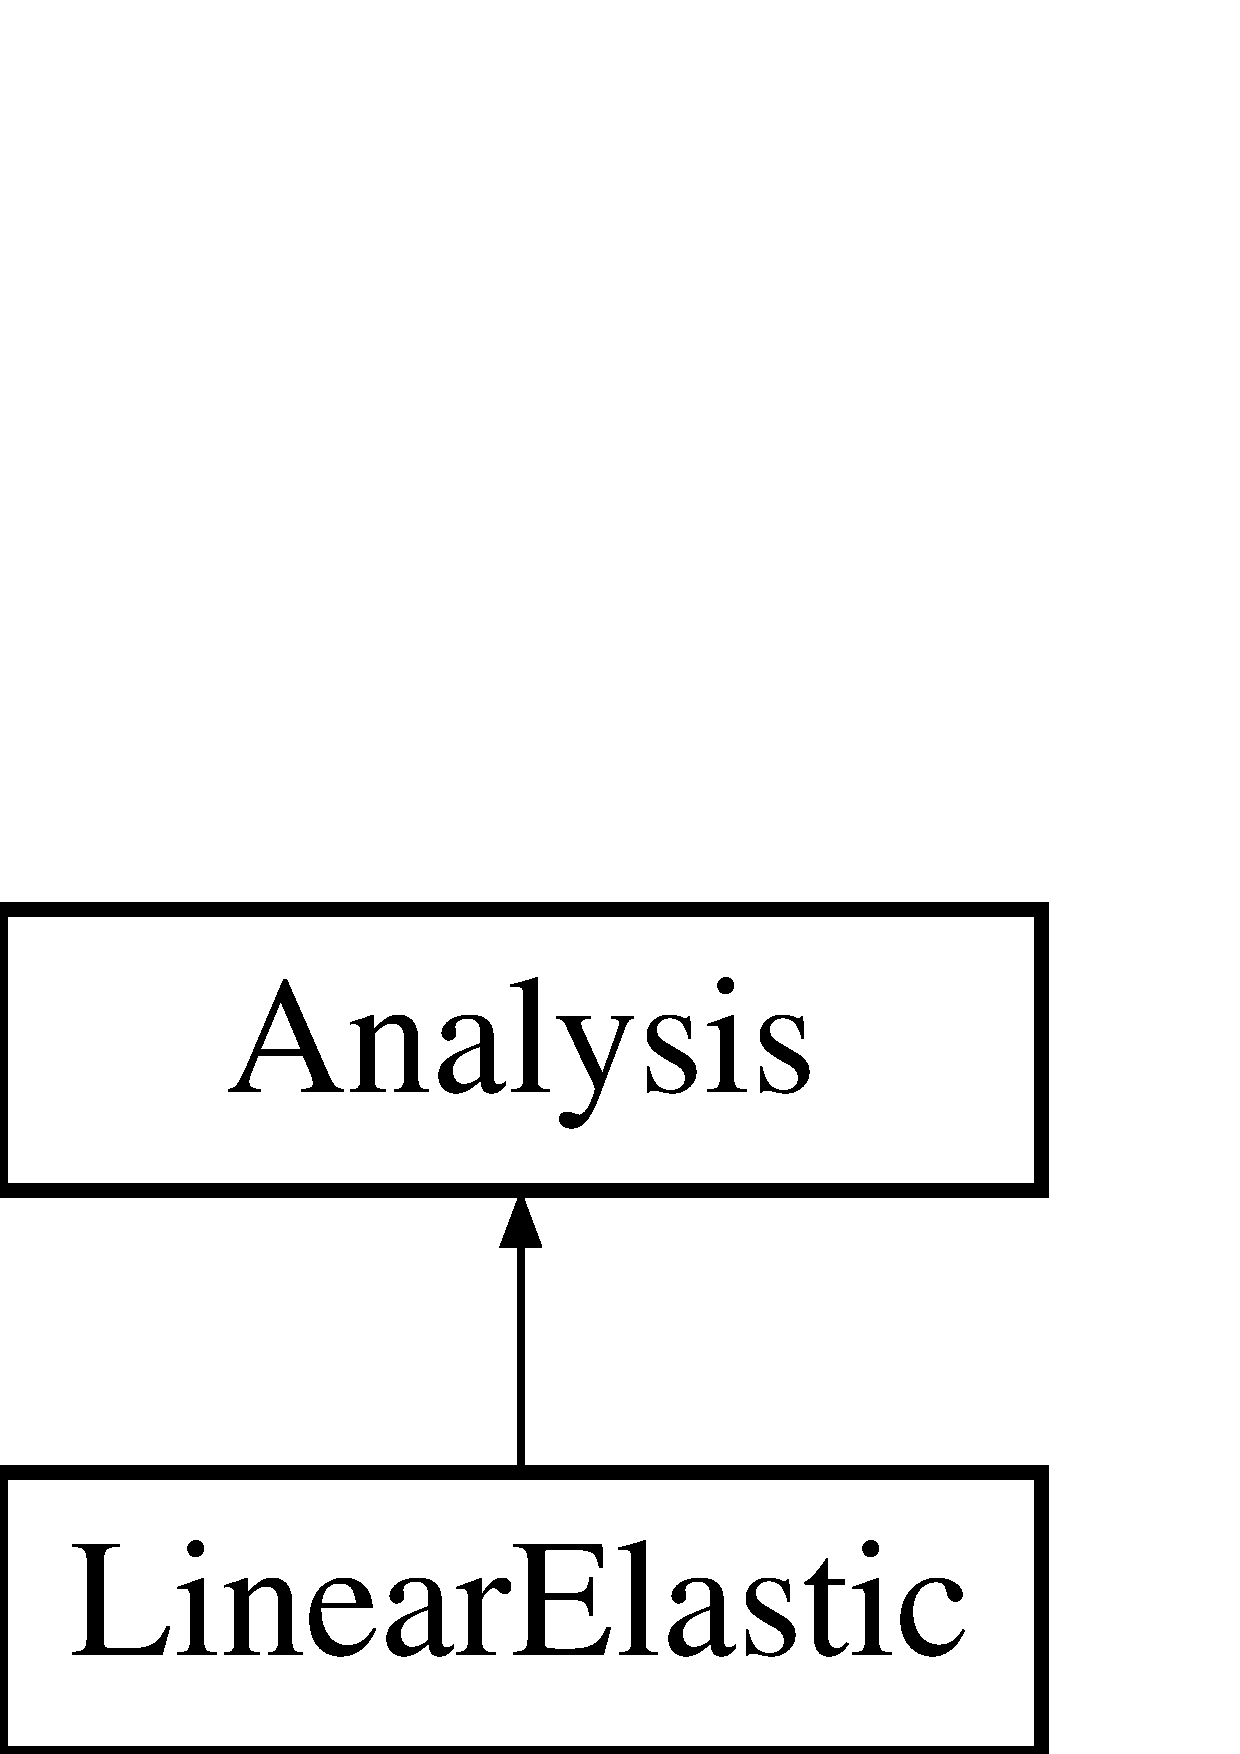
\includegraphics[height=2.000000cm]{class_linear_elastic}
\end{center}
\end{figure}
\subsection*{Public Member Functions}
\begin{DoxyCompactItemize}
\item 
\mbox{\Hypertarget{class_linear_elastic_af1b56916522c2f91f4f6e817ed63cfbe}\label{class_linear_elastic_af1b56916522c2f91f4f6e817ed63cfbe}} 
{\bfseries Linear\+Elastic} (std\+::string const \&file\+Name)
\item 
\mbox{\Hypertarget{class_linear_elastic_add96aa6fdb7cbbbcef2dca1f31ca0779}\label{class_linear_elastic_add96aa6fdb7cbbbcef2dca1f31ca0779}} 
void \mbox{\hyperlink{class_linear_elastic_add96aa6fdb7cbbbcef2dca1f31ca0779}{solve\+Disp}} ()
\begin{DoxyCompactList}\small\item\em Solve for nodal displacement using different approaches. \end{DoxyCompactList}\end{DoxyCompactItemize}
\subsection*{Additional Inherited Members}


The documentation for this class was generated from the following files\+:\begin{DoxyCompactItemize}
\item 
\mbox{\hyperlink{_linear_elastic_8h}{Linear\+Elastic.\+h}}\item 
\mbox{\hyperlink{_linear_elastic_8cpp}{Linear\+Elastic.\+cpp}}\end{DoxyCompactItemize}

\hypertarget{class_material}{}\section{Material Class Reference}
\label{class_material}\index{Material@{Material}}


\mbox{\hyperlink{class_material}{Material}} class for storing the engineering properties of elements.  




{\ttfamily \#include $<$Material.\+h$>$}

\subsection*{Public Member Functions}
\begin{DoxyCompactItemize}
\item 
\mbox{\hyperlink{class_material_aa37938070139aa60f67d245d3b0ce352}{Material}} (const std\+::vector$<$ double $>$ \&properties)
\begin{DoxyCompactList}\small\item\em Custom constructor to create an element material. \end{DoxyCompactList}\item 
const Matrix\+Xd \& \mbox{\hyperlink{class_material_abaae85c04f84374421337e2bf140ec0a}{E\+Matrix}} () const
\begin{DoxyCompactList}\small\item\em Get the stress-\/strain constitutive matrix of the element. \end{DoxyCompactList}\item 
const Vector2d \& \mbox{\hyperlink{class_material_a5995e3b7d8063f670e33f2fcd7315928}{body\+Force}} () const
\begin{DoxyCompactList}\small\item\em Get the body force to be used in the load condition. \end{DoxyCompactList}\item 
const Vector\+Xd \& \mbox{\hyperlink{class_material_ae84dc6468819487050db131b589ffb95}{thermal\+Strain}} () const
\begin{DoxyCompactList}\small\item\em Get the thermal strain to be used in the stress computation. \end{DoxyCompactList}\end{DoxyCompactItemize}
\subsection*{Protected Attributes}
\begin{DoxyCompactItemize}
\item 
\mbox{\Hypertarget{class_material_a505d8c136dd80cdfb78e2b9f6468be46}\label{class_material_a505d8c136dd80cdfb78e2b9f6468be46}} 
double \mbox{\hyperlink{class_material_a505d8c136dd80cdfb78e2b9f6468be46}{modulus\+\_\+}}
\begin{DoxyCompactList}\small\item\em The modulus. \end{DoxyCompactList}\item 
\mbox{\Hypertarget{class_material_ac49581c3474d4106011a211f063c5b1d}\label{class_material_ac49581c3474d4106011a211f063c5b1d}} 
double \mbox{\hyperlink{class_material_ac49581c3474d4106011a211f063c5b1d}{poisson\+Ratio\+\_\+}}
\begin{DoxyCompactList}\small\item\em The Poisson\textquotesingle{}s ratio. \end{DoxyCompactList}\item 
\mbox{\Hypertarget{class_material_ad8eb23b2b0c134635888be8e3b6a824c}\label{class_material_ad8eb23b2b0c134635888be8e3b6a824c}} 
Matrix\+Xd \mbox{\hyperlink{class_material_ad8eb23b2b0c134635888be8e3b6a824c}{E\+\_\+}}
\begin{DoxyCompactList}\small\item\em The 4-\/by-\/4 stress-\/strain constitutive matrix sigma = E $\ast$ e. \end{DoxyCompactList}\item 
\mbox{\Hypertarget{class_material_af29cbdb8e4fa9fbc0e04cf89b72a2c18}\label{class_material_af29cbdb8e4fa9fbc0e04cf89b72a2c18}} 
Vector2d \mbox{\hyperlink{class_material_af29cbdb8e4fa9fbc0e04cf89b72a2c18}{body\+Force\+\_\+}}
\begin{DoxyCompactList}\small\item\em The body force (unit weight) \end{DoxyCompactList}\item 
\mbox{\Hypertarget{class_material_a51b256107e8ddc53c6b12b90b481034d}\label{class_material_a51b256107e8ddc53c6b12b90b481034d}} 
double \mbox{\hyperlink{class_material_a51b256107e8ddc53c6b12b90b481034d}{thermal\+Coeff\+\_\+}}
\begin{DoxyCompactList}\small\item\em The coefficient of thermal effect. \end{DoxyCompactList}\item 
\mbox{\Hypertarget{class_material_a4c80934742a60ab5414e92c4b97d08ca}\label{class_material_a4c80934742a60ab5414e92c4b97d08ca}} 
double \mbox{\hyperlink{class_material_a4c80934742a60ab5414e92c4b97d08ca}{delta\+T\+\_\+}}
\begin{DoxyCompactList}\small\item\em The temperature change (assume same across the entire element) \end{DoxyCompactList}\item 
\mbox{\Hypertarget{class_material_a26c58d90ad30a49acb8342196166ab41}\label{class_material_a26c58d90ad30a49acb8342196166ab41}} 
Vector\+Xd \mbox{\hyperlink{class_material_a26c58d90ad30a49acb8342196166ab41}{thermal\+Strain\+\_\+}}
\begin{DoxyCompactList}\small\item\em The thermal strain. \end{DoxyCompactList}\end{DoxyCompactItemize}


\subsection{Detailed Description}
\mbox{\hyperlink{class_material}{Material}} class for storing the engineering properties of elements. 



\subsection{Constructor \& Destructor Documentation}
\mbox{\Hypertarget{class_material_aa37938070139aa60f67d245d3b0ce352}\label{class_material_aa37938070139aa60f67d245d3b0ce352}} 
\index{Material@{Material}!Material@{Material}}
\index{Material@{Material}!Material@{Material}}
\subsubsection{\texorpdfstring{Material()}{Material()}}
{\footnotesize\ttfamily Material\+::\+Material (\begin{DoxyParamCaption}\item[{const std\+::vector$<$ double $>$ \&}]{properties }\end{DoxyParamCaption})}



Custom constructor to create an element material. 


\begin{DoxyParams}{Parameters}
{\em properties} & A list of the property parameters. \\
\hline
\end{DoxyParams}


\subsection{Member Function Documentation}
\mbox{\Hypertarget{class_material_a5995e3b7d8063f670e33f2fcd7315928}\label{class_material_a5995e3b7d8063f670e33f2fcd7315928}} 
\index{Material@{Material}!body\+Force@{body\+Force}}
\index{body\+Force@{body\+Force}!Material@{Material}}
\subsubsection{\texorpdfstring{body\+Force()}{bodyForce()}}
{\footnotesize\ttfamily const Vector2d \& Material\+::body\+Force (\begin{DoxyParamCaption}{ }\end{DoxyParamCaption}) const}



Get the body force to be used in the load condition. 

\begin{DoxyReturn}{Returns}
The body force as a 2-\/by-\/1 vector for 2D axisymmetric problem. 
\end{DoxyReturn}
\mbox{\Hypertarget{class_material_abaae85c04f84374421337e2bf140ec0a}\label{class_material_abaae85c04f84374421337e2bf140ec0a}} 
\index{Material@{Material}!E\+Matrix@{E\+Matrix}}
\index{E\+Matrix@{E\+Matrix}!Material@{Material}}
\subsubsection{\texorpdfstring{E\+Matrix()}{EMatrix()}}
{\footnotesize\ttfamily const Matrix\+Xd \& Material\+::\+E\+Matrix (\begin{DoxyParamCaption}{ }\end{DoxyParamCaption}) const}



Get the stress-\/strain constitutive matrix of the element. 

\begin{DoxyReturn}{Returns}
The 4-\/by-\/4 E matrix. 
\end{DoxyReturn}
\mbox{\Hypertarget{class_material_ae84dc6468819487050db131b589ffb95}\label{class_material_ae84dc6468819487050db131b589ffb95}} 
\index{Material@{Material}!thermal\+Strain@{thermal\+Strain}}
\index{thermal\+Strain@{thermal\+Strain}!Material@{Material}}
\subsubsection{\texorpdfstring{thermal\+Strain()}{thermalStrain()}}
{\footnotesize\ttfamily const Vector\+Xd \& Material\+::thermal\+Strain (\begin{DoxyParamCaption}{ }\end{DoxyParamCaption}) const}



Get the thermal strain to be used in the stress computation. 

\begin{DoxyReturn}{Returns}
The thermal strain as a 4-\/by-\/1 vector for 2D axisymmetric problem. 
\end{DoxyReturn}


The documentation for this class was generated from the following files\+:\begin{DoxyCompactItemize}
\item 
\mbox{\hyperlink{_material_8h}{Material.\+h}}\item 
\mbox{\hyperlink{_material_8cpp}{Material.\+cpp}}\end{DoxyCompactItemize}

\hypertarget{class_mesh}{}\section{Mesh Class Reference}
\label{class_mesh}\index{Mesh@{Mesh}}
\subsection*{Public Member Functions}
\begin{DoxyCompactItemize}
\item 
\mbox{\Hypertarget{class_mesh_a2af137f1571af89172b9c102302c416b}\label{class_mesh_a2af137f1571af89172b9c102302c416b}} 
\mbox{\hyperlink{class_mesh_a2af137f1571af89172b9c102302c416b}{Mesh}} ()
\begin{DoxyCompactList}\small\item\em Default constructor for \mbox{\hyperlink{class_mesh}{Mesh}}. \end{DoxyCompactList}\item 
\mbox{\hyperlink{class_mesh_af9ff79e2003cfde74b16266cd8113acf}{Mesh}} (std\+::string const \&file\+Name)
\begin{DoxyCompactList}\small\item\em Custom constructor to create a mesh with given file name. \end{DoxyCompactList}\item 
\mbox{\Hypertarget{class_mesh_a5efe4da1a4c0971cfb037bd70304c303}\label{class_mesh_a5efe4da1a4c0971cfb037bd70304c303}} 
\mbox{\hyperlink{class_mesh_a5efe4da1a4c0971cfb037bd70304c303}{$\sim$\+Mesh}} ()
\begin{DoxyCompactList}\small\item\em Destructor for \mbox{\hyperlink{class_mesh}{Mesh}}. \end{DoxyCompactList}\item 
void \mbox{\hyperlink{class_mesh_a519813e103dbb3fb1739a2c40b3e1153}{read\+From\+File}} (std\+::string const \&file\+Name)
\begin{DoxyCompactList}\small\item\em Read in all the information and build the mesh. \end{DoxyCompactList}\item 
const int \& \mbox{\hyperlink{class_mesh_a6a535f67f00ed39f945aaa1e8039a277}{node\+Count}} () const
\begin{DoxyCompactList}\small\item\em Get the total number of the nodes. \end{DoxyCompactList}\item 
const int \& \mbox{\hyperlink{class_mesh_aa1b2aafa40bd4b335e9bf6306e482881}{element\+Count}} () const
\begin{DoxyCompactList}\small\item\em Get the total number of the elements. \end{DoxyCompactList}\item 
\mbox{\hyperlink{class_node}{Node}} $\ast$const \mbox{\hyperlink{class_mesh_a071a8dfe15c00fcabc9c4071306487d4}{get\+Node}} (const int \&index) const
\begin{DoxyCompactList}\small\item\em Get the node at given zero-\/based index. \end{DoxyCompactList}\item 
\mbox{\hyperlink{class_element}{Element}} $\ast$const \mbox{\hyperlink{class_mesh_ada2ae7b8640a3999780d7e738ee4154e}{get\+Element}} (const int \&index) const
\begin{DoxyCompactList}\small\item\em Get the element at given zero-\/based index. \end{DoxyCompactList}\item 
\mbox{\hyperlink{class_node}{Node}} $\ast$$\ast$const \mbox{\hyperlink{class_mesh_ae596a597115563fb308d99e5e15a62e6}{node\+Array}} () const
\begin{DoxyCompactList}\small\item\em Get the node array. \end{DoxyCompactList}\item 
\mbox{\hyperlink{class_element}{Element}} $\ast$$\ast$const \mbox{\hyperlink{class_mesh_a042cc2ef19b7090f830b915721818181}{element\+Array}} () const
\begin{DoxyCompactList}\small\item\em Get the element array. \end{DoxyCompactList}\end{DoxyCompactItemize}
\subsection*{Public Attributes}
\begin{DoxyCompactItemize}
\item 
std\+::vector$<$ int $>$ \mbox{\hyperlink{class_mesh_a5a1c5739ef85c8f9071f689e790b5251}{boundary\+Node\+List}}
\begin{DoxyCompactList}\small\item\em \mbox{\hyperlink{class_a}{A}} list of the degree of freedom that are at boundary. \end{DoxyCompactList}\item 
\mbox{\Hypertarget{class_mesh_ab331f3e3efeb2934c202b07db8a6c1a5}\label{class_mesh_ab331f3e3efeb2934c202b07db8a6c1a5}} 
std\+::vector$<$ double $>$ \mbox{\hyperlink{class_mesh_ab331f3e3efeb2934c202b07db8a6c1a5}{boundary\+Value}}
\begin{DoxyCompactList}\small\item\em The boundary values corresponding to the D\+OF list above. \end{DoxyCompactList}\item 
\mbox{\Hypertarget{class_mesh_ad54254084b97877bb4d0f9d9d9cbb380}\label{class_mesh_ad54254084b97877bb4d0f9d9d9cbb380}} 
std\+::vector$<$ int $>$ \mbox{\hyperlink{class_mesh_ad54254084b97877bb4d0f9d9d9cbb380}{load\+Node\+List}}
\begin{DoxyCompactList}\small\item\em \mbox{\hyperlink{class_a}{A}} D\+OF list (see above) of the node with applied load. \end{DoxyCompactList}\item 
\mbox{\Hypertarget{class_mesh_a688adb457f52ffa939f53f22afae697e}\label{class_mesh_a688adb457f52ffa939f53f22afae697e}} 
std\+::vector$<$ double $>$ \mbox{\hyperlink{class_mesh_a688adb457f52ffa939f53f22afae697e}{load\+Value}}
\begin{DoxyCompactList}\small\item\em The load values at the node. \end{DoxyCompactList}\end{DoxyCompactItemize}


\subsection{Detailed Description}


Definition at line 20 of file Mesh.\+h.



\subsection{Constructor \& Destructor Documentation}
\mbox{\Hypertarget{class_mesh_af9ff79e2003cfde74b16266cd8113acf}\label{class_mesh_af9ff79e2003cfde74b16266cd8113acf}} 
\index{Mesh@{Mesh}!Mesh@{Mesh}}
\index{Mesh@{Mesh}!Mesh@{Mesh}}
\subsubsection{\texorpdfstring{Mesh()}{Mesh()}}
{\footnotesize\ttfamily Mesh\+::\+Mesh (\begin{DoxyParamCaption}\item[{std\+::string const \&}]{file\+Name }\end{DoxyParamCaption})}



Custom constructor to create a mesh with given file name. 


\begin{DoxyParams}{Parameters}
{\em file\+Name} & The path to the input file. \\
\hline
\end{DoxyParams}


Definition at line 25 of file Mesh.\+cpp.



\subsection{Member Function Documentation}
\mbox{\Hypertarget{class_mesh_a042cc2ef19b7090f830b915721818181}\label{class_mesh_a042cc2ef19b7090f830b915721818181}} 
\index{Mesh@{Mesh}!element\+Array@{element\+Array}}
\index{element\+Array@{element\+Array}!Mesh@{Mesh}}
\subsubsection{\texorpdfstring{element\+Array()}{elementArray()}}
{\footnotesize\ttfamily \mbox{\hyperlink{class_element}{Element}} $\ast$$\ast$const Mesh\+::element\+Array (\begin{DoxyParamCaption}{ }\end{DoxyParamCaption}) const}



Get the element array. 

\begin{DoxyReturn}{Returns}
\mbox{\hyperlink{class_a}{A}} pointer to the element pool.
\end{DoxyReturn}
\begin{DoxyNote}{Note}
There are two ways to query a node/element\+: mesh.\+node\+Array()\mbox{[}i\mbox{]} OR mesh.\+get\+Node(i) 
\end{DoxyNote}


Definition at line 221 of file Mesh.\+cpp.

\mbox{\Hypertarget{class_mesh_aa1b2aafa40bd4b335e9bf6306e482881}\label{class_mesh_aa1b2aafa40bd4b335e9bf6306e482881}} 
\index{Mesh@{Mesh}!element\+Count@{element\+Count}}
\index{element\+Count@{element\+Count}!Mesh@{Mesh}}
\subsubsection{\texorpdfstring{element\+Count()}{elementCount()}}
{\footnotesize\ttfamily const int \& Mesh\+::element\+Count (\begin{DoxyParamCaption}{ }\end{DoxyParamCaption}) const}



Get the total number of the elements. 

\begin{DoxyReturn}{Returns}
The total number of the elements. 
\end{DoxyReturn}


Definition at line 201 of file Mesh.\+cpp.

\mbox{\Hypertarget{class_mesh_ada2ae7b8640a3999780d7e738ee4154e}\label{class_mesh_ada2ae7b8640a3999780d7e738ee4154e}} 
\index{Mesh@{Mesh}!get\+Element@{get\+Element}}
\index{get\+Element@{get\+Element}!Mesh@{Mesh}}
\subsubsection{\texorpdfstring{get\+Element()}{getElement()}}
{\footnotesize\ttfamily \mbox{\hyperlink{class_element}{Element}} $\ast$const Mesh\+::get\+Element (\begin{DoxyParamCaption}\item[{const int \&}]{index }\end{DoxyParamCaption}) const}



Get the element at given zero-\/based index. 


\begin{DoxyParams}{Parameters}
{\em index} & The index for query. \\
\hline
\end{DoxyParams}
\begin{DoxyReturn}{Returns}
\mbox{\hyperlink{class_a}{A}} pointer to the element being queried. 
\end{DoxyReturn}


Definition at line 211 of file Mesh.\+cpp.

\mbox{\Hypertarget{class_mesh_a071a8dfe15c00fcabc9c4071306487d4}\label{class_mesh_a071a8dfe15c00fcabc9c4071306487d4}} 
\index{Mesh@{Mesh}!get\+Node@{get\+Node}}
\index{get\+Node@{get\+Node}!Mesh@{Mesh}}
\subsubsection{\texorpdfstring{get\+Node()}{getNode()}}
{\footnotesize\ttfamily \mbox{\hyperlink{class_node}{Node}} $\ast$const Mesh\+::get\+Node (\begin{DoxyParamCaption}\item[{const int \&}]{index }\end{DoxyParamCaption}) const}



Get the node at given zero-\/based index. 


\begin{DoxyParams}{Parameters}
{\em index} & The index for query. \\
\hline
\end{DoxyParams}
\begin{DoxyReturn}{Returns}
\mbox{\hyperlink{class_a}{A}} pointer to the node being queried. 
\end{DoxyReturn}


Definition at line 206 of file Mesh.\+cpp.

\mbox{\Hypertarget{class_mesh_ae596a597115563fb308d99e5e15a62e6}\label{class_mesh_ae596a597115563fb308d99e5e15a62e6}} 
\index{Mesh@{Mesh}!node\+Array@{node\+Array}}
\index{node\+Array@{node\+Array}!Mesh@{Mesh}}
\subsubsection{\texorpdfstring{node\+Array()}{nodeArray()}}
{\footnotesize\ttfamily \mbox{\hyperlink{class_node}{Node}} $\ast$$\ast$const Mesh\+::node\+Array (\begin{DoxyParamCaption}{ }\end{DoxyParamCaption}) const}



Get the node array. 

\begin{DoxyReturn}{Returns}
\mbox{\hyperlink{class_a}{A}} pointer to the node pool. 
\end{DoxyReturn}


Definition at line 216 of file Mesh.\+cpp.

\mbox{\Hypertarget{class_mesh_a6a535f67f00ed39f945aaa1e8039a277}\label{class_mesh_a6a535f67f00ed39f945aaa1e8039a277}} 
\index{Mesh@{Mesh}!node\+Count@{node\+Count}}
\index{node\+Count@{node\+Count}!Mesh@{Mesh}}
\subsubsection{\texorpdfstring{node\+Count()}{nodeCount()}}
{\footnotesize\ttfamily const int \& Mesh\+::node\+Count (\begin{DoxyParamCaption}{ }\end{DoxyParamCaption}) const}



Get the total number of the nodes. 

\begin{DoxyReturn}{Returns}
The total number of the nodes. 
\end{DoxyReturn}


Definition at line 196 of file Mesh.\+cpp.

\mbox{\Hypertarget{class_mesh_a519813e103dbb3fb1739a2c40b3e1153}\label{class_mesh_a519813e103dbb3fb1739a2c40b3e1153}} 
\index{Mesh@{Mesh}!read\+From\+File@{read\+From\+File}}
\index{read\+From\+File@{read\+From\+File}!Mesh@{Mesh}}
\subsubsection{\texorpdfstring{read\+From\+File()}{readFromFile()}}
{\footnotesize\ttfamily void Mesh\+::read\+From\+File (\begin{DoxyParamCaption}\item[{std\+::string const \&}]{file\+Name }\end{DoxyParamCaption})}



Read in all the information and build the mesh. 


\begin{DoxyParams}{Parameters}
{\em file\+Name} & The path to the input file. \\
\hline
\end{DoxyParams}


Definition at line 45 of file Mesh.\+cpp.



\subsection{Member Data Documentation}
\mbox{\Hypertarget{class_mesh_a5a1c5739ef85c8f9071f689e790b5251}\label{class_mesh_a5a1c5739ef85c8f9071f689e790b5251}} 
\index{Mesh@{Mesh}!boundary\+Node\+List@{boundary\+Node\+List}}
\index{boundary\+Node\+List@{boundary\+Node\+List}!Mesh@{Mesh}}
\subsubsection{\texorpdfstring{boundary\+Node\+List}{boundaryNodeList}}
{\footnotesize\ttfamily std\+::vector$<$int$>$ Mesh\+::boundary\+Node\+List}



\mbox{\hyperlink{class_a}{A}} list of the degree of freedom that are at boundary. 

\begin{DoxyNote}{Note}
Actually this is not N\+O\+DE list, but degree of freedom list, e.\+g., if node 1,2 are X\&Y fixed, node 4 is x fixed, then the D\+OF list is (2,3 $\vert$ 4,5 $\vert$ 8) and the boundary value list below is (0,0,0,0,0). 
\end{DoxyNote}


Definition at line 100 of file Mesh.\+h.



The documentation for this class was generated from the following files\+:\begin{DoxyCompactItemize}
\item 
\mbox{\hyperlink{_mesh_8h}{Mesh.\+h}}\item 
\mbox{\hyperlink{_mesh_8cpp}{Mesh.\+cpp}}\end{DoxyCompactItemize}

\hypertarget{class_node}{}\section{Node Class Reference}
\label{class_node}\index{Node@{Node}}
\subsection*{Public Member Functions}
\begin{DoxyCompactItemize}
\item 
\mbox{\Hypertarget{class_node_ad7a34779cad45d997bfd6d3d8043c75f}\label{class_node_ad7a34779cad45d997bfd6d3d8043c75f}} 
\mbox{\hyperlink{class_node_ad7a34779cad45d997bfd6d3d8043c75f}{Node}} ()
\begin{DoxyCompactList}\small\item\em Default constructor for \mbox{\hyperlink{class_node}{Node}}. \end{DoxyCompactList}\item 
\mbox{\hyperlink{class_node_a7dd5e46921c9aa573f8167e1f3d0acaa}{Node}} (const int \&index, const double \&x, const double \&y)
\begin{DoxyCompactList}\small\item\em Custom constructor to create a node with given node coordinates. \end{DoxyCompactList}\item 
\mbox{\Hypertarget{class_node_aef463e59f7af71d83b6392089c27bcba}\label{class_node_aef463e59f7af71d83b6392089c27bcba}} 
\mbox{\hyperlink{class_node_aef463e59f7af71d83b6392089c27bcba}{Node}} (\mbox{\hyperlink{class_node}{Node}} const \&other)
\begin{DoxyCompactList}\small\item\em Copy constructor. \end{DoxyCompactList}\item 
\mbox{\Hypertarget{class_node_a0abaefd98651b6cdba055d4644360170}\label{class_node_a0abaefd98651b6cdba055d4644360170}} 
\mbox{\hyperlink{class_node}{Node}} const  \& \mbox{\hyperlink{class_node_a0abaefd98651b6cdba055d4644360170}{operator=}} (\mbox{\hyperlink{class_node}{Node}} const \&other)
\begin{DoxyCompactList}\small\item\em Assignment operator. \end{DoxyCompactList}\item 
\mbox{\Hypertarget{class_node_aa0840c3cb5c7159be6d992adecd2097c}\label{class_node_aa0840c3cb5c7159be6d992adecd2097c}} 
\mbox{\hyperlink{class_node_aa0840c3cb5c7159be6d992adecd2097c}{$\sim$\+Node}} ()
\begin{DoxyCompactList}\small\item\em Destructor. \end{DoxyCompactList}\item 
void \mbox{\hyperlink{class_node_acea5ca0209b0c5cffa48d564320e4d56}{set\+Global\+Coord}} (const double \&x, const double \&y)
\begin{DoxyCompactList}\small\item\em Assign the initial global coordinates (r,z) of the node. \end{DoxyCompactList}\item 
void \mbox{\hyperlink{class_node_a9703bb2540dbc410edd3a168a6c51cd6}{set\+Disp}} (const double \&u, const double \&v)
\begin{DoxyCompactList}\small\item\em Assign the final solved displacements (u,v) at the node. \end{DoxyCompactList}\item 
void \mbox{\hyperlink{class_node_a261921c1143a8dfb7f7f7f454ce827e3}{set\+Force}} (const double \&Fx, const double \&Fy)
\begin{DoxyCompactList}\small\item\em Assign the final solved force (Fx, Fy) at the node. \end{DoxyCompactList}\item 
void \mbox{\hyperlink{class_node_a31e8635344b96ab5df9e6df5e5466533}{set\+Strain\+And\+Stress}} (const Vector\+Xd \&strain, const Vector\+Xd \&stress)
\begin{DoxyCompactList}\small\item\em Cumulate the stress and strain values at this node by summing up the values from each adjacent element. \end{DoxyCompactList}\item 
const Vector\+Xd \& \mbox{\hyperlink{class_node_a8a8d206f3e35f105b9a5e45d83e32126}{average\+Strain}} ()
\begin{DoxyCompactList}\small\item\em Average the strain vector at this node. \end{DoxyCompactList}\item 
const Vector\+Xd \& \mbox{\hyperlink{class_node_afe17aee2d10e0a65e48ad892a160f287}{average\+Stress}} ()
\begin{DoxyCompactList}\small\item\em Average the stress vector at this node. \end{DoxyCompactList}\item 
const int \& \mbox{\hyperlink{class_node_a8266479b3d82c502d7b4abc5afccb8c0}{get\+Index}} () const
\begin{DoxyCompactList}\small\item\em Get the index of this node. \end{DoxyCompactList}\item 
const Vector2d \& \mbox{\hyperlink{class_node_ab0129116eb1cff646bd53b8120cd34e6}{get\+Global\+Coord}} () const
\begin{DoxyCompactList}\small\item\em Get the initial global coordinates (r,z) of the node. \end{DoxyCompactList}\item 
const Vector2d \& \mbox{\hyperlink{class_node_a2024b690427f7840b18dc429d4acba7d}{get\+Disp}} () const
\begin{DoxyCompactList}\small\item\em Get the solved displacements (u,v) at the node. \end{DoxyCompactList}\item 
const Vector2d \& \mbox{\hyperlink{class_node_acb1728229a234694419ecda6ad5928c4}{get\+Force}} () const
\begin{DoxyCompactList}\small\item\em Get the solved force (Fx, Fy) at the node. \end{DoxyCompactList}\end{DoxyCompactItemize}


\subsection{Detailed Description}


Definition at line 19 of file Node.\+h.



\subsection{Constructor \& Destructor Documentation}
\mbox{\Hypertarget{class_node_a7dd5e46921c9aa573f8167e1f3d0acaa}\label{class_node_a7dd5e46921c9aa573f8167e1f3d0acaa}} 
\index{Node@{Node}!Node@{Node}}
\index{Node@{Node}!Node@{Node}}
\subsubsection{\texorpdfstring{Node()}{Node()}}
{\footnotesize\ttfamily Node\+::\+Node (\begin{DoxyParamCaption}\item[{const int \&}]{index,  }\item[{const double \&}]{x,  }\item[{const double \&}]{y }\end{DoxyParamCaption})}



Custom constructor to create a node with given node coordinates. 


\begin{DoxyParams}{Parameters}
{\em index} & The index number of current node. \\
\hline
{\em x} & The global x-\/coordinate of the node. \\
\hline
{\em y} & The global y-\/coordinate of the node. \\
\hline
\end{DoxyParams}
\begin{DoxyNote}{Note}
All pass-\/by-\/ref. 
\end{DoxyNote}


Definition at line 17 of file Node.\+cpp.



\subsection{Member Function Documentation}
\mbox{\Hypertarget{class_node_a8a8d206f3e35f105b9a5e45d83e32126}\label{class_node_a8a8d206f3e35f105b9a5e45d83e32126}} 
\index{Node@{Node}!average\+Strain@{average\+Strain}}
\index{average\+Strain@{average\+Strain}!Node@{Node}}
\subsubsection{\texorpdfstring{average\+Strain()}{averageStrain()}}
{\footnotesize\ttfamily const Vector\+Xd \& Node\+::average\+Strain (\begin{DoxyParamCaption}{ }\end{DoxyParamCaption})}



Average the strain vector at this node. 

\begin{DoxyReturn}{Returns}
The average strain vector.
\end{DoxyReturn}
\begin{DoxyNote}{Note}
\mbox{\hyperlink{class_node}{Node}} objects are dynamically allocated on heap memory, so we can return-\/by-\/ref. 
\end{DoxyNote}


Definition at line 79 of file Node.\+cpp.

\mbox{\Hypertarget{class_node_afe17aee2d10e0a65e48ad892a160f287}\label{class_node_afe17aee2d10e0a65e48ad892a160f287}} 
\index{Node@{Node}!average\+Stress@{average\+Stress}}
\index{average\+Stress@{average\+Stress}!Node@{Node}}
\subsubsection{\texorpdfstring{average\+Stress()}{averageStress()}}
{\footnotesize\ttfamily const Vector\+Xd \& Node\+::average\+Stress (\begin{DoxyParamCaption}{ }\end{DoxyParamCaption})}



Average the stress vector at this node. 

\begin{DoxyReturn}{Returns}
The average stress vector. 
\end{DoxyReturn}


Definition at line 84 of file Node.\+cpp.

\mbox{\Hypertarget{class_node_a2024b690427f7840b18dc429d4acba7d}\label{class_node_a2024b690427f7840b18dc429d4acba7d}} 
\index{Node@{Node}!get\+Disp@{get\+Disp}}
\index{get\+Disp@{get\+Disp}!Node@{Node}}
\subsubsection{\texorpdfstring{get\+Disp()}{getDisp()}}
{\footnotesize\ttfamily const Vector2d \& Node\+::get\+Disp (\begin{DoxyParamCaption}{ }\end{DoxyParamCaption}) const}



Get the solved displacements (u,v) at the node. 

\begin{DoxyReturn}{Returns}
The displacements. 
\end{DoxyReturn}


Definition at line 99 of file Node.\+cpp.

\mbox{\Hypertarget{class_node_acb1728229a234694419ecda6ad5928c4}\label{class_node_acb1728229a234694419ecda6ad5928c4}} 
\index{Node@{Node}!get\+Force@{get\+Force}}
\index{get\+Force@{get\+Force}!Node@{Node}}
\subsubsection{\texorpdfstring{get\+Force()}{getForce()}}
{\footnotesize\ttfamily const Vector2d \& Node\+::get\+Force (\begin{DoxyParamCaption}{ }\end{DoxyParamCaption}) const}



Get the solved force (Fx, Fy) at the node. 

\begin{DoxyReturn}{Returns}
The forces. 
\end{DoxyReturn}


Definition at line 104 of file Node.\+cpp.

\mbox{\Hypertarget{class_node_ab0129116eb1cff646bd53b8120cd34e6}\label{class_node_ab0129116eb1cff646bd53b8120cd34e6}} 
\index{Node@{Node}!get\+Global\+Coord@{get\+Global\+Coord}}
\index{get\+Global\+Coord@{get\+Global\+Coord}!Node@{Node}}
\subsubsection{\texorpdfstring{get\+Global\+Coord()}{getGlobalCoord()}}
{\footnotesize\ttfamily const Vector2d \& Node\+::get\+Global\+Coord (\begin{DoxyParamCaption}{ }\end{DoxyParamCaption}) const}



Get the initial global coordinates (r,z) of the node. 

\begin{DoxyReturn}{Returns}
The global coordinates. 
\end{DoxyReturn}


Definition at line 94 of file Node.\+cpp.

\mbox{\Hypertarget{class_node_a8266479b3d82c502d7b4abc5afccb8c0}\label{class_node_a8266479b3d82c502d7b4abc5afccb8c0}} 
\index{Node@{Node}!get\+Index@{get\+Index}}
\index{get\+Index@{get\+Index}!Node@{Node}}
\subsubsection{\texorpdfstring{get\+Index()}{getIndex()}}
{\footnotesize\ttfamily const int \& Node\+::get\+Index (\begin{DoxyParamCaption}{ }\end{DoxyParamCaption}) const}



Get the index of this node. 

\begin{DoxyReturn}{Returns}
The index. 
\end{DoxyReturn}


Definition at line 89 of file Node.\+cpp.

\mbox{\Hypertarget{class_node_a9703bb2540dbc410edd3a168a6c51cd6}\label{class_node_a9703bb2540dbc410edd3a168a6c51cd6}} 
\index{Node@{Node}!set\+Disp@{set\+Disp}}
\index{set\+Disp@{set\+Disp}!Node@{Node}}
\subsubsection{\texorpdfstring{set\+Disp()}{setDisp()}}
{\footnotesize\ttfamily void Node\+::set\+Disp (\begin{DoxyParamCaption}\item[{const double \&}]{u,  }\item[{const double \&}]{v }\end{DoxyParamCaption})}



Assign the final solved displacements (u,v) at the node. 


\begin{DoxyParams}{Parameters}
{\em u} & The x-\/displacement at the node. \\
\hline
{\em v} & The y-\/displacement at the node. \\
\hline
\end{DoxyParams}


Definition at line 62 of file Node.\+cpp.

\mbox{\Hypertarget{class_node_a261921c1143a8dfb7f7f7f454ce827e3}\label{class_node_a261921c1143a8dfb7f7f7f454ce827e3}} 
\index{Node@{Node}!set\+Force@{set\+Force}}
\index{set\+Force@{set\+Force}!Node@{Node}}
\subsubsection{\texorpdfstring{set\+Force()}{setForce()}}
{\footnotesize\ttfamily void Node\+::set\+Force (\begin{DoxyParamCaption}\item[{const double \&}]{Fx,  }\item[{const double \&}]{Fy }\end{DoxyParamCaption})}



Assign the final solved force (Fx, Fy) at the node. 


\begin{DoxyParams}{Parameters}
{\em Fx} & The x-\/force applied the node. \\
\hline
{\em Fy} & The y-\/force applied the node. \\
\hline
\end{DoxyParams}


Definition at line 67 of file Node.\+cpp.

\mbox{\Hypertarget{class_node_acea5ca0209b0c5cffa48d564320e4d56}\label{class_node_acea5ca0209b0c5cffa48d564320e4d56}} 
\index{Node@{Node}!set\+Global\+Coord@{set\+Global\+Coord}}
\index{set\+Global\+Coord@{set\+Global\+Coord}!Node@{Node}}
\subsubsection{\texorpdfstring{set\+Global\+Coord()}{setGlobalCoord()}}
{\footnotesize\ttfamily void Node\+::set\+Global\+Coord (\begin{DoxyParamCaption}\item[{const double \&}]{x,  }\item[{const double \&}]{y }\end{DoxyParamCaption})}



Assign the initial global coordinates (r,z) of the node. 


\begin{DoxyParams}{Parameters}
{\em x} & The global x-\/coordinate of the node. \\
\hline
{\em y} & The global y-\/coordinate of the node. \\
\hline
\end{DoxyParams}


Definition at line 57 of file Node.\+cpp.

\mbox{\Hypertarget{class_node_a31e8635344b96ab5df9e6df5e5466533}\label{class_node_a31e8635344b96ab5df9e6df5e5466533}} 
\index{Node@{Node}!set\+Strain\+And\+Stress@{set\+Strain\+And\+Stress}}
\index{set\+Strain\+And\+Stress@{set\+Strain\+And\+Stress}!Node@{Node}}
\subsubsection{\texorpdfstring{set\+Strain\+And\+Stress()}{setStrainAndStress()}}
{\footnotesize\ttfamily void Node\+::set\+Strain\+And\+Stress (\begin{DoxyParamCaption}\item[{const Vector\+Xd \&}]{strain,  }\item[{const Vector\+Xd \&}]{stress }\end{DoxyParamCaption})}



Cumulate the stress and strain values at this node by summing up the values from each adjacent element. 


\begin{DoxyParams}{Parameters}
{\em strain} & The strain vector to be added to this node. The form is\+: \mbox{[}e(r), e(theta), e(z), gamma(rz)\mbox{]}. \\
\hline
{\em stress} & The stress vector to be added to this node. The form is\+: \mbox{[}s(r), s(theta), s(z), t(rz)\mbox{]}.\\
\hline
\end{DoxyParams}
\begin{DoxyNote}{Note}
This is an internal step for computing the averaged strain and stress at each node. The cumulative value will be averaged later. 
\end{DoxyNote}


Definition at line 72 of file Node.\+cpp.



The documentation for this class was generated from the following files\+:\begin{DoxyCompactItemize}
\item 
\mbox{\hyperlink{_node_8h}{Node.\+h}}\item 
\mbox{\hyperlink{_node_8cpp}{Node.\+cpp}}\end{DoxyCompactItemize}

\hypertarget{class_shape}{}\section{Shape Class Reference}
\label{class_shape}\index{Shape@{Shape}}
Inheritance diagram for Shape\+:\begin{figure}[H]
\begin{center}
\leavevmode
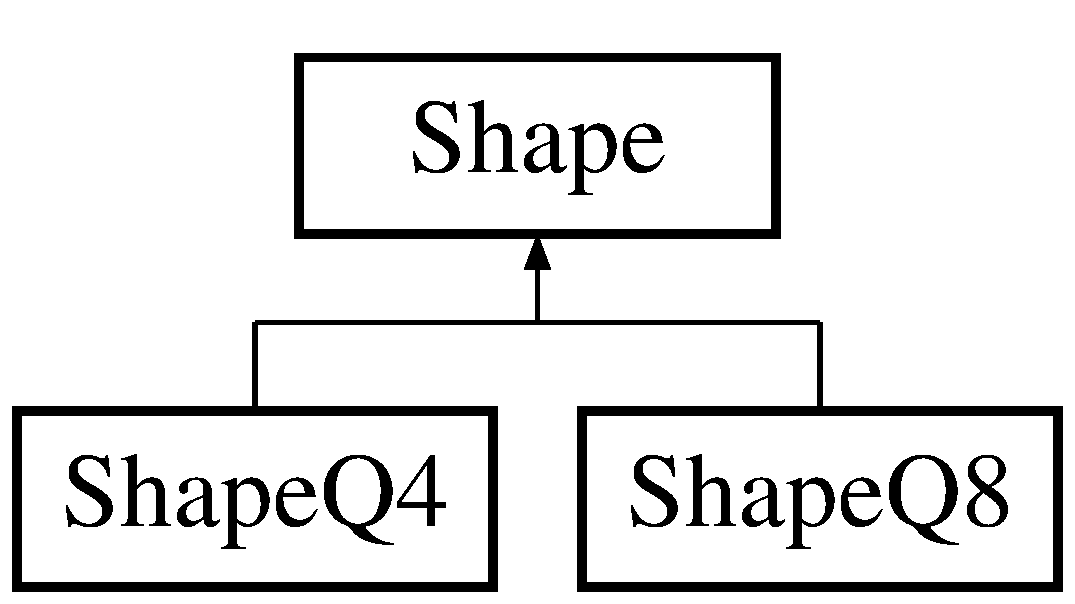
\includegraphics[height=2.000000cm]{class_shape}
\end{center}
\end{figure}
\subsection*{Public Member Functions}
\begin{DoxyCompactItemize}
\item 
\mbox{\hyperlink{class_shape_aab720d4a61d7f8016ab9a72bab846cbe}{Shape}} (const int \&nodes, const int \&gaussians, const int \&edges, const int \&edge\+Nodes, const int \&edge\+Gaussians)
\begin{DoxyCompactList}\small\item\em Constructor for \mbox{\hyperlink{class_shape}{Shape}} class. \end{DoxyCompactList}\item 
\mbox{\Hypertarget{class_shape_ac3b9fc48965274893f25b18aa14ba665}\label{class_shape_ac3b9fc48965274893f25b18aa14ba665}} 
virtual \mbox{\hyperlink{class_shape_ac3b9fc48965274893f25b18aa14ba665}{$\sim$\+Shape}} ()
\begin{DoxyCompactList}\small\item\em Destructor for \mbox{\hyperlink{class_shape}{Shape}}. \end{DoxyCompactList}\item 
virtual Vector\+Xd \mbox{\hyperlink{class_shape_a0e0400bca54c29b5097c84ace51ecc7b}{function\+Vec}} (const Vector2d \&point) const =0
\begin{DoxyCompactList}\small\item\em Compute the shape Function N in a column vector at a given point. \end{DoxyCompactList}\item 
virtual Matrix\+Xd \mbox{\hyperlink{class_shape_a7a2dc7c642bdea2a1359e3795fd9414d}{function\+Mat}} (const Vector2d \&point) const =0
\begin{DoxyCompactList}\small\item\em Stack and interleave the shape Function N above into a matrix for the convenience of stiffness matrix computation. \end{DoxyCompactList}\item 
virtual Matrix\+Xd \mbox{\hyperlink{class_shape_a29de5d31e0fa74a4d1067f6d14cd94ed}{function\+Deriv}} (const Vector2d \&point) const =0
\begin{DoxyCompactList}\small\item\em Compute the local derivatives d\+N/d(xi) and d\+N/d(eta) of the shape function at a given point in isoparametric coordinates. \end{DoxyCompactList}\item 
virtual Vector\+Xd \mbox{\hyperlink{class_shape_aeb6b5b956ca89b571d17ee7e140bb689}{edge\+Function\+Vec}} (const double \&point) const =0
\begin{DoxyCompactList}\small\item\em Compute the edge shape Function N in a column vector at a given point. \end{DoxyCompactList}\item 
virtual Matrix\+Xd \mbox{\hyperlink{class_shape_ac9854f15377ea07c97be16049e3058d5}{edge\+Function\+Mat}} (const double \&point) const =0
\begin{DoxyCompactList}\small\item\em Stack and interleave the edge shape Function N above into a matrix. \end{DoxyCompactList}\item 
virtual Vector\+Xd \mbox{\hyperlink{class_shape_a652164292592de3157eb4021f43c9305}{edge\+Function\+Deriv}} (const double \&point) const =0
\begin{DoxyCompactList}\small\item\em Compute the local derivatives d\+N/dx of the edge shape function at a given point in isoparametric coordinates. \end{DoxyCompactList}\item 
const std\+::vector$<$ Vector2d $>$ \& \mbox{\hyperlink{class_shape_a8d53e88ab51926dc57177c56c3fde714}{gaussian\+Pt}} () const
\begin{DoxyCompactList}\small\item\em Get the gaussian integration points to be used in load distribution and stress/strain computation. \end{DoxyCompactList}\item 
const Vector2d \& \mbox{\hyperlink{class_shape_a66cd2cc62229a4757a5d0eeeb36197de}{gaussian\+Pt}} (const int \&i) const
\begin{DoxyCompactList}\small\item\em Get the ith gaussian integration points. \end{DoxyCompactList}\item 
const std\+::vector$<$ double $>$ \& \mbox{\hyperlink{class_shape_aa6112974b77db75f70e5a7367d30ed78}{gaussian\+Wt}} () const
\begin{DoxyCompactList}\small\item\em Get the gaussian integration weights to be used in load distribution and stress/strain computation. \end{DoxyCompactList}\item 
const double \& \mbox{\hyperlink{class_shape_ab59598c42a7ecbe41998820bf43e1307}{gaussian\+Wt}} (const int \&i) const
\begin{DoxyCompactList}\small\item\em Get the ith gaussian weights. \end{DoxyCompactList}\item 
const Vector\+Xd \& \mbox{\hyperlink{class_shape_a69936bb268e5a1547f5e5838dde5bcdf}{function\+Vec}} (const int \&i) const
\begin{DoxyCompactList}\small\item\em Get pre-\/cached shape function (vector form) at certin Gaussian point. \end{DoxyCompactList}\item 
const Matrix\+Xd \& \mbox{\hyperlink{class_shape_a96b2b268631566142aa054211ddd9655}{function\+Mat}} (const int \&i) const
\begin{DoxyCompactList}\small\item\em Get pre-\/cached shape function (matrix form) at certin Gaussian point. \end{DoxyCompactList}\item 
const Matrix\+Xd \& \mbox{\hyperlink{class_shape_abb3d4512095e82bcaf821385e1952336}{function\+Deriv}} (const int \&i) const
\begin{DoxyCompactList}\small\item\em Get pre-\/cached shape function derivative matrix at certin Gaussian point. \end{DoxyCompactList}\item 
const Vector\+Xd \& \mbox{\hyperlink{class_shape_a1d79b0ac86d547e06121eec43cbdea2b}{edge\+Function\+Vec}} (const int \&i) const
\begin{DoxyCompactList}\small\item\em Get pre-\/cached edge shape function (vector form) at certin Gaussian point. \end{DoxyCompactList}\item 
const Matrix\+Xd \& \mbox{\hyperlink{class_shape_a5d6e400458f3381b3adeeac34839e401}{edge\+Function\+Mat}} (const int \&i) const
\begin{DoxyCompactList}\small\item\em Get pre-\/cached edge shape function (matrix form) at certin Gaussian point. \end{DoxyCompactList}\item 
const Vector\+Xd \& \mbox{\hyperlink{class_shape_adb82ef67f86561caa0cebdb4abb7342a}{edge\+Function\+Deriv}} (const int \&i) const
\begin{DoxyCompactList}\small\item\em Get pre-\/cached edge shape function derivative matrix at certin Gaussian point. \end{DoxyCompactList}\item 
const std\+::vector$<$ double $>$ \& \mbox{\hyperlink{class_shape_af004504284fc26fee888906a13a6fab2}{edge\+Gaussian\+Pt}} () const
\begin{DoxyCompactList}\small\item\em Get the edge gaussian integration points to be used in load distribution and stress/strain computation. \end{DoxyCompactList}\item 
const std\+::vector$<$ double $>$ \& \mbox{\hyperlink{class_shape_a651a829c004900fe28c9bdadf0939306}{edge\+Gaussian\+Wt}} () const
\begin{DoxyCompactList}\small\item\em Get the edge gaussian integration weights to be used in load distribution and stress/strain computation. \end{DoxyCompactList}\item 
const std\+::vector$<$ int $>$ \& \mbox{\hyperlink{class_shape_a3d0c3331bae4cad90eb8b5de8f095140}{edge}} (const int \&i) const
\begin{DoxyCompactList}\small\item\em Get the node index of ith edge. \end{DoxyCompactList}\end{DoxyCompactItemize}
\subsection*{Protected Member Functions}
\begin{DoxyCompactItemize}
\item 
\mbox{\Hypertarget{class_shape_aea3b1ebc3bc64d488e8d55877fcd5ec7}\label{class_shape_aea3b1ebc3bc64d488e8d55877fcd5ec7}} 
void \mbox{\hyperlink{class_shape_aea3b1ebc3bc64d488e8d55877fcd5ec7}{\+\_\+cache\+Shape}} ()
\begin{DoxyCompactList}\small\item\em Private helper function for Pre-\/caching the shape functions at Gaussian integration points. \end{DoxyCompactList}\end{DoxyCompactItemize}
\subsection*{Protected Attributes}
\begin{DoxyCompactItemize}
\item 
\mbox{\Hypertarget{class_shape_a8bf4568013144202ee5152bd3cb615ce}\label{class_shape_a8bf4568013144202ee5152bd3cb615ce}} 
int \mbox{\hyperlink{class_shape_a8bf4568013144202ee5152bd3cb615ce}{num\+Nodes\+\_\+}}
\begin{DoxyCompactList}\small\item\em The number of nodes of this element type. \end{DoxyCompactList}\item 
\mbox{\Hypertarget{class_shape_a23d18bcf055ecd99e5754bb749ca28b5}\label{class_shape_a23d18bcf055ecd99e5754bb749ca28b5}} 
std\+::vector$<$ Vector2d $>$ \mbox{\hyperlink{class_shape_a23d18bcf055ecd99e5754bb749ca28b5}{node\+Coord\+\_\+}}
\begin{DoxyCompactList}\small\item\em The local isoparametric coordinates (xi,eta) of the element nodes. \end{DoxyCompactList}\item 
\mbox{\Hypertarget{class_shape_aa12dd7e6505e22036ab61b1b0a3debd3}\label{class_shape_aa12dd7e6505e22036ab61b1b0a3debd3}} 
int \mbox{\hyperlink{class_shape_aa12dd7e6505e22036ab61b1b0a3debd3}{num\+Gaussian\+Pts\+\_\+}}
\begin{DoxyCompactList}\small\item\em The number of Gaussian integration points of the element. \end{DoxyCompactList}\item 
\mbox{\Hypertarget{class_shape_ab8ca49604843e6153730bb2138aa1255}\label{class_shape_ab8ca49604843e6153730bb2138aa1255}} 
std\+::vector$<$ Vector2d $>$ \mbox{\hyperlink{class_shape_ab8ca49604843e6153730bb2138aa1255}{gaussian\+Pt\+\_\+}}
\begin{DoxyCompactList}\small\item\em An array of the coordinates of 2D Gaussian integration points. \end{DoxyCompactList}\item 
\mbox{\Hypertarget{class_shape_a0a81426ae65a0216eb099ab63cd4691b}\label{class_shape_a0a81426ae65a0216eb099ab63cd4691b}} 
std\+::vector$<$ double $>$ \mbox{\hyperlink{class_shape_a0a81426ae65a0216eb099ab63cd4691b}{gaussian\+Wt\+\_\+}}
\begin{DoxyCompactList}\small\item\em An array of the weights of Gaussian integration points. \end{DoxyCompactList}\item 
\mbox{\Hypertarget{class_shape_ab20d7fb49963b09d1c294f28c6e5295b}\label{class_shape_ab20d7fb49963b09d1c294f28c6e5295b}} 
std\+::vector$<$ Vector\+Xd $>$ \mbox{\hyperlink{class_shape_ab20d7fb49963b09d1c294f28c6e5295b}{shape\+Vec\+\_\+}}
\begin{DoxyCompactList}\small\item\em An array of the shape functions (vector form) at all Gaussian points. \end{DoxyCompactList}\item 
\mbox{\Hypertarget{class_shape_a9eab26923dfc3dbe90dbcab164e63f28}\label{class_shape_a9eab26923dfc3dbe90dbcab164e63f28}} 
std\+::vector$<$ Matrix\+Xd $>$ \mbox{\hyperlink{class_shape_a9eab26923dfc3dbe90dbcab164e63f28}{shape\+Mat\+\_\+}}
\begin{DoxyCompactList}\small\item\em An array of the shape functions (stacked matrix form) at all Gaussian points. \end{DoxyCompactList}\item 
\mbox{\Hypertarget{class_shape_a11bf0927166d002fb730889275d608ea}\label{class_shape_a11bf0927166d002fb730889275d608ea}} 
std\+::vector$<$ Matrix\+Xd $>$ \mbox{\hyperlink{class_shape_a11bf0927166d002fb730889275d608ea}{shape\+Deriv\+\_\+}}
\begin{DoxyCompactList}\small\item\em An array of the derivatives of shape function (stacked matrix form) at all Gaussian points. \end{DoxyCompactList}\item 
\mbox{\Hypertarget{class_shape_a48cc39a592761dce468c50c9bf0d77fe}\label{class_shape_a48cc39a592761dce468c50c9bf0d77fe}} 
int \mbox{\hyperlink{class_shape_a48cc39a592761dce468c50c9bf0d77fe}{num\+Edges\+\_\+}}
\begin{DoxyCompactList}\small\item\em The number of edges of this element type. \end{DoxyCompactList}\item 
\mbox{\Hypertarget{class_shape_a0de5974df65f16f324f3c1f3fcfaee81}\label{class_shape_a0de5974df65f16f324f3c1f3fcfaee81}} 
int \mbox{\hyperlink{class_shape_a0de5974df65f16f324f3c1f3fcfaee81}{num\+Edge\+Nodes\+\_\+}}
\begin{DoxyCompactList}\small\item\em The number of nodes an edge has. \end{DoxyCompactList}\item 
\mbox{\Hypertarget{class_shape_a5834a3c81b025002ff7325c7e030f2cf}\label{class_shape_a5834a3c81b025002ff7325c7e030f2cf}} 
std\+::vector$<$ std\+::vector$<$ int $>$ $>$ \mbox{\hyperlink{class_shape_a5834a3c81b025002ff7325c7e030f2cf}{edge\+List\+\_\+}}
\begin{DoxyCompactList}\small\item\em An array of the edges with its node indices. \end{DoxyCompactList}\item 
\mbox{\Hypertarget{class_shape_a974a69473ea089377e2a45295306142d}\label{class_shape_a974a69473ea089377e2a45295306142d}} 
int \mbox{\hyperlink{class_shape_a974a69473ea089377e2a45295306142d}{num\+Edge\+Gaussian\+Pts\+\_\+}}
\begin{DoxyCompactList}\small\item\em The number of Gaussian integration points of an edge. \end{DoxyCompactList}\item 
\mbox{\Hypertarget{class_shape_a607f731349b6bc16fe81a08289c7e452}\label{class_shape_a607f731349b6bc16fe81a08289c7e452}} 
std\+::vector$<$ double $>$ \mbox{\hyperlink{class_shape_a607f731349b6bc16fe81a08289c7e452}{edge\+Gaussian\+Pt\+\_\+}}
\begin{DoxyCompactList}\small\item\em An array of the coordinates of the 1D Gaussian points of an edge. \end{DoxyCompactList}\item 
\mbox{\Hypertarget{class_shape_ac44104e1110f94f376419f62c76d4428}\label{class_shape_ac44104e1110f94f376419f62c76d4428}} 
std\+::vector$<$ double $>$ \mbox{\hyperlink{class_shape_ac44104e1110f94f376419f62c76d4428}{edge\+Gaussian\+Wt\+\_\+}}
\begin{DoxyCompactList}\small\item\em An array of the weights of Gaussian points of an edge. \end{DoxyCompactList}\item 
\mbox{\Hypertarget{class_shape_ac668fd1eff17dac98616158e1cab17fa}\label{class_shape_ac668fd1eff17dac98616158e1cab17fa}} 
std\+::vector$<$ Vector\+Xd $>$ \mbox{\hyperlink{class_shape_ac668fd1eff17dac98616158e1cab17fa}{edge\+Shape\+Vec\+\_\+}}
\begin{DoxyCompactList}\small\item\em An array of the edge shape functions (vector form) at Gaussian points. \end{DoxyCompactList}\item 
\mbox{\Hypertarget{class_shape_af81a39560f87d14ba1a50c9eda7fff12}\label{class_shape_af81a39560f87d14ba1a50c9eda7fff12}} 
std\+::vector$<$ Matrix\+Xd $>$ \mbox{\hyperlink{class_shape_af81a39560f87d14ba1a50c9eda7fff12}{edge\+Shape\+Mat\+\_\+}}
\begin{DoxyCompactList}\small\item\em An array of the edge shape functions (stacked matrix form) at Gaussian points. \end{DoxyCompactList}\item 
\mbox{\Hypertarget{class_shape_a5cc69ac9662365109eabd0a193e48781}\label{class_shape_a5cc69ac9662365109eabd0a193e48781}} 
std\+::vector$<$ Vector\+Xd $>$ \mbox{\hyperlink{class_shape_a5cc69ac9662365109eabd0a193e48781}{edge\+Shape\+Deriv\+\_\+}}
\begin{DoxyCompactList}\small\item\em An array of the derivatives of edge shape function (vector form) at Gaussian points. \end{DoxyCompactList}\end{DoxyCompactItemize}


\subsection{Constructor \& Destructor Documentation}
\mbox{\Hypertarget{class_shape_aab720d4a61d7f8016ab9a72bab846cbe}\label{class_shape_aab720d4a61d7f8016ab9a72bab846cbe}} 
\index{Shape@{Shape}!Shape@{Shape}}
\index{Shape@{Shape}!Shape@{Shape}}
\subsubsection{\texorpdfstring{Shape()}{Shape()}}
{\footnotesize\ttfamily Shape\+::\+Shape (\begin{DoxyParamCaption}\item[{const int \&}]{nodes,  }\item[{const int \&}]{gaussians,  }\item[{const int \&}]{edges,  }\item[{const int \&}]{edge\+Nodes,  }\item[{const int \&}]{edge\+Gaussians }\end{DoxyParamCaption})}



Constructor for \mbox{\hyperlink{class_shape}{Shape}} class. 


\begin{DoxyParams}{Parameters}
{\em nodes} & Number of nodes of this shape of element. \\
\hline
{\em gaussians} & Number of Gaussian integration points of this shape of element. \\
\hline
{\em edges} & Number of edges of this shape of element. \\
\hline
{\em edge\+Nodes} & Number of nodes each edge consists of. \\
\hline
{\em edge\+Gaussians} & Number of Gaussian intergration points at each edge.\\
\hline
\end{DoxyParams}
\begin{DoxyNote}{Note}
The information about edges and its integration are specified at initialization because no assumption or generic forms can be made. It should leave the decision for user to define and select different types of integration scheme (normal integration, reduced integration, etc.). Additionally, no assumption can be made because the shape could be triangular, quadrilateral, or any arbitrary form so that no predetermined \mbox{\hyperlink{class_node}{Node}} number-\/\+Edge number-\/\+Gaussian point number relation exists. 
\end{DoxyNote}


\subsection{Member Function Documentation}
\mbox{\Hypertarget{class_shape_a3d0c3331bae4cad90eb8b5de8f095140}\label{class_shape_a3d0c3331bae4cad90eb8b5de8f095140}} 
\index{Shape@{Shape}!edge@{edge}}
\index{edge@{edge}!Shape@{Shape}}
\subsubsection{\texorpdfstring{edge()}{edge()}}
{\footnotesize\ttfamily const std\+::vector$<$ int $>$ \& Shape\+::edge (\begin{DoxyParamCaption}\item[{const int \&}]{i }\end{DoxyParamCaption}) const}



Get the node index of ith edge. 


\begin{DoxyParams}{Parameters}
{\em i} & The zero-\/based edge index being queried. \\
\hline
\end{DoxyParams}
\begin{DoxyReturn}{Returns}
An array of node indices belonging to ith edge. 
\end{DoxyReturn}
\mbox{\Hypertarget{class_shape_a652164292592de3157eb4021f43c9305}\label{class_shape_a652164292592de3157eb4021f43c9305}} 
\index{Shape@{Shape}!edge\+Function\+Deriv@{edge\+Function\+Deriv}}
\index{edge\+Function\+Deriv@{edge\+Function\+Deriv}!Shape@{Shape}}
\subsubsection{\texorpdfstring{edge\+Function\+Deriv()}{edgeFunctionDeriv()}\hspace{0.1cm}{\footnotesize\ttfamily [1/2]}}
{\footnotesize\ttfamily virtual Vector\+Xd Shape\+::edge\+Function\+Deriv (\begin{DoxyParamCaption}\item[{const double \&}]{point }\end{DoxyParamCaption}) const\hspace{0.3cm}{\ttfamily [pure virtual]}}



Compute the local derivatives d\+N/dx of the edge shape function at a given point in isoparametric coordinates. 


\begin{DoxyParams}{Parameters}
{\em point} & A 1D point x at which the edge shape function to be evaluated. Pass-\/by-\/ref. \\
\hline
\end{DoxyParams}
\begin{DoxyReturn}{Returns}
The edge shape function derivatives dN as a column vector at given point. 
\end{DoxyReturn}


Implemented in \mbox{\hyperlink{class_shape_q8_a81582d03b2fc79a8a5705111ad85163f}{Shape\+Q8}}.

\mbox{\Hypertarget{class_shape_adb82ef67f86561caa0cebdb4abb7342a}\label{class_shape_adb82ef67f86561caa0cebdb4abb7342a}} 
\index{Shape@{Shape}!edge\+Function\+Deriv@{edge\+Function\+Deriv}}
\index{edge\+Function\+Deriv@{edge\+Function\+Deriv}!Shape@{Shape}}
\subsubsection{\texorpdfstring{edge\+Function\+Deriv()}{edgeFunctionDeriv()}\hspace{0.1cm}{\footnotesize\ttfamily [2/2]}}
{\footnotesize\ttfamily const Vector\+Xd \& Shape\+::edge\+Function\+Deriv (\begin{DoxyParamCaption}\item[{const int \&}]{i }\end{DoxyParamCaption}) const}



Get pre-\/cached edge shape function derivative matrix at certin Gaussian point. 


\begin{DoxyParams}{Parameters}
{\em i} & The index of Gaussian points to be queried. \\
\hline
\end{DoxyParams}
\begin{DoxyReturn}{Returns}
The derivatives of shape function dN as a column vector at Gaussian point i. 
\end{DoxyReturn}
\mbox{\Hypertarget{class_shape_ac9854f15377ea07c97be16049e3058d5}\label{class_shape_ac9854f15377ea07c97be16049e3058d5}} 
\index{Shape@{Shape}!edge\+Function\+Mat@{edge\+Function\+Mat}}
\index{edge\+Function\+Mat@{edge\+Function\+Mat}!Shape@{Shape}}
\subsubsection{\texorpdfstring{edge\+Function\+Mat()}{edgeFunctionMat()}\hspace{0.1cm}{\footnotesize\ttfamily [1/2]}}
{\footnotesize\ttfamily virtual Matrix\+Xd Shape\+::edge\+Function\+Mat (\begin{DoxyParamCaption}\item[{const double \&}]{point }\end{DoxyParamCaption}) const\hspace{0.3cm}{\ttfamily [pure virtual]}}



Stack and interleave the edge shape Function N above into a matrix. 


\begin{DoxyParams}{Parameters}
{\em point} & A 1D point x at which the edge shape function to be evaluated. Pass-\/by-\/ref. \\
\hline
\end{DoxyParams}
\begin{DoxyReturn}{Returns}
The stacked and interleaved edge shape function N as a matrix at given point. 
\end{DoxyReturn}


Implemented in \mbox{\hyperlink{class_shape_q8_a0c52ac2dbeb9297c11e03c664d4750b7}{Shape\+Q8}}.

\mbox{\Hypertarget{class_shape_a5d6e400458f3381b3adeeac34839e401}\label{class_shape_a5d6e400458f3381b3adeeac34839e401}} 
\index{Shape@{Shape}!edge\+Function\+Mat@{edge\+Function\+Mat}}
\index{edge\+Function\+Mat@{edge\+Function\+Mat}!Shape@{Shape}}
\subsubsection{\texorpdfstring{edge\+Function\+Mat()}{edgeFunctionMat()}\hspace{0.1cm}{\footnotesize\ttfamily [2/2]}}
{\footnotesize\ttfamily const Matrix\+Xd \& Shape\+::edge\+Function\+Mat (\begin{DoxyParamCaption}\item[{const int \&}]{i }\end{DoxyParamCaption}) const}



Get pre-\/cached edge shape function (matrix form) at certin Gaussian point. 


\begin{DoxyParams}{Parameters}
{\em i} & The index of Gaussian points to be queried. \\
\hline
\end{DoxyParams}
\begin{DoxyReturn}{Returns}
The edge shape function N as a matrix (interleaved) at Gaussian point i. 
\end{DoxyReturn}
\mbox{\Hypertarget{class_shape_aeb6b5b956ca89b571d17ee7e140bb689}\label{class_shape_aeb6b5b956ca89b571d17ee7e140bb689}} 
\index{Shape@{Shape}!edge\+Function\+Vec@{edge\+Function\+Vec}}
\index{edge\+Function\+Vec@{edge\+Function\+Vec}!Shape@{Shape}}
\subsubsection{\texorpdfstring{edge\+Function\+Vec()}{edgeFunctionVec()}\hspace{0.1cm}{\footnotesize\ttfamily [1/2]}}
{\footnotesize\ttfamily virtual Vector\+Xd Shape\+::edge\+Function\+Vec (\begin{DoxyParamCaption}\item[{const double \&}]{point }\end{DoxyParamCaption}) const\hspace{0.3cm}{\ttfamily [pure virtual]}}



Compute the edge shape Function N in a column vector at a given point. 


\begin{DoxyParams}{Parameters}
{\em point} & A 1D point x at which the edge shape function to be evaluated. Pass-\/by-\/ref. \\
\hline
\end{DoxyParams}
\begin{DoxyReturn}{Returns}
The edge shape function N as a column vector at given point. 
\end{DoxyReturn}


Implemented in \mbox{\hyperlink{class_shape_q8_a6d5e89cd06d6639e599215686553adbe}{Shape\+Q8}}.

\mbox{\Hypertarget{class_shape_a1d79b0ac86d547e06121eec43cbdea2b}\label{class_shape_a1d79b0ac86d547e06121eec43cbdea2b}} 
\index{Shape@{Shape}!edge\+Function\+Vec@{edge\+Function\+Vec}}
\index{edge\+Function\+Vec@{edge\+Function\+Vec}!Shape@{Shape}}
\subsubsection{\texorpdfstring{edge\+Function\+Vec()}{edgeFunctionVec()}\hspace{0.1cm}{\footnotesize\ttfamily [2/2]}}
{\footnotesize\ttfamily const Vector\+Xd \& Shape\+::edge\+Function\+Vec (\begin{DoxyParamCaption}\item[{const int \&}]{i }\end{DoxyParamCaption}) const}



Get pre-\/cached edge shape function (vector form) at certin Gaussian point. 


\begin{DoxyParams}{Parameters}
{\em i} & The index of Gaussian points to be queried. \\
\hline
\end{DoxyParams}
\begin{DoxyReturn}{Returns}
The edge shape function N as a column vector at Gaussian point i. 
\end{DoxyReturn}
\mbox{\Hypertarget{class_shape_af004504284fc26fee888906a13a6fab2}\label{class_shape_af004504284fc26fee888906a13a6fab2}} 
\index{Shape@{Shape}!edge\+Gaussian\+Pt@{edge\+Gaussian\+Pt}}
\index{edge\+Gaussian\+Pt@{edge\+Gaussian\+Pt}!Shape@{Shape}}
\subsubsection{\texorpdfstring{edge\+Gaussian\+Pt()}{edgeGaussianPt()}}
{\footnotesize\ttfamily const std\+::vector$<$ double $>$ \& Shape\+::edge\+Gaussian\+Pt (\begin{DoxyParamCaption}{ }\end{DoxyParamCaption}) const}



Get the edge gaussian integration points to be used in load distribution and stress/strain computation. 

\begin{DoxyReturn}{Returns}
An array of 1D points. 
\end{DoxyReturn}
\mbox{\Hypertarget{class_shape_a651a829c004900fe28c9bdadf0939306}\label{class_shape_a651a829c004900fe28c9bdadf0939306}} 
\index{Shape@{Shape}!edge\+Gaussian\+Wt@{edge\+Gaussian\+Wt}}
\index{edge\+Gaussian\+Wt@{edge\+Gaussian\+Wt}!Shape@{Shape}}
\subsubsection{\texorpdfstring{edge\+Gaussian\+Wt()}{edgeGaussianWt()}}
{\footnotesize\ttfamily const std\+::vector$<$ double $>$ \& Shape\+::edge\+Gaussian\+Wt (\begin{DoxyParamCaption}{ }\end{DoxyParamCaption}) const}



Get the edge gaussian integration weights to be used in load distribution and stress/strain computation. 

\begin{DoxyReturn}{Returns}
An array of weight values. 
\end{DoxyReturn}
\mbox{\Hypertarget{class_shape_a29de5d31e0fa74a4d1067f6d14cd94ed}\label{class_shape_a29de5d31e0fa74a4d1067f6d14cd94ed}} 
\index{Shape@{Shape}!function\+Deriv@{function\+Deriv}}
\index{function\+Deriv@{function\+Deriv}!Shape@{Shape}}
\subsubsection{\texorpdfstring{function\+Deriv()}{functionDeriv()}\hspace{0.1cm}{\footnotesize\ttfamily [1/2]}}
{\footnotesize\ttfamily virtual Matrix\+Xd Shape\+::function\+Deriv (\begin{DoxyParamCaption}\item[{const Vector2d \&}]{point }\end{DoxyParamCaption}) const\hspace{0.3cm}{\ttfamily [pure virtual]}}



Compute the local derivatives d\+N/d(xi) and d\+N/d(eta) of the shape function at a given point in isoparametric coordinates. 

If n is the number of nodes of this element type, then this function will returns a 2-\/by-\/n matrix\+:

\mbox{[} d\+N1(x)/d(xi) d\+N2(x)/d(xi) ... d\+Nn(x)/d(xi) \mbox{]} \mbox{[} d\+N1(x)/d(eta) d\+N2(x)/d(eta) ... d\+Nn(x)/d(eta) \mbox{]}


\begin{DoxyParams}{Parameters}
{\em point} & A 2D point x(r,z) at which the shape function to be evaluated. Pass-\/by-\/ref. \\
\hline
\end{DoxyParams}
\begin{DoxyReturn}{Returns}
The stacked and interleaved shape function derivatives dN as a matrix at given point. 
\end{DoxyReturn}


Implemented in \mbox{\hyperlink{class_shape_q8_a49ab65aee22c0b8df4b9cb24b973a882}{Shape\+Q8}}, and \mbox{\hyperlink{class_shape_q4_a23e45399e8867f74c47eb41a30328e3e}{Shape\+Q4}}.

\mbox{\Hypertarget{class_shape_abb3d4512095e82bcaf821385e1952336}\label{class_shape_abb3d4512095e82bcaf821385e1952336}} 
\index{Shape@{Shape}!function\+Deriv@{function\+Deriv}}
\index{function\+Deriv@{function\+Deriv}!Shape@{Shape}}
\subsubsection{\texorpdfstring{function\+Deriv()}{functionDeriv()}\hspace{0.1cm}{\footnotesize\ttfamily [2/2]}}
{\footnotesize\ttfamily const Matrix\+Xd \& Shape\+::function\+Deriv (\begin{DoxyParamCaption}\item[{const int \&}]{i }\end{DoxyParamCaption}) const}



Get pre-\/cached shape function derivative matrix at certin Gaussian point. 


\begin{DoxyParams}{Parameters}
{\em i} & The index of Gaussian points to be queried. \\
\hline
\end{DoxyParams}
\begin{DoxyReturn}{Returns}
The derivatives of shape function dN as a matrix (not interleaved) at Gaussian point i. 
\end{DoxyReturn}
\mbox{\Hypertarget{class_shape_a7a2dc7c642bdea2a1359e3795fd9414d}\label{class_shape_a7a2dc7c642bdea2a1359e3795fd9414d}} 
\index{Shape@{Shape}!function\+Mat@{function\+Mat}}
\index{function\+Mat@{function\+Mat}!Shape@{Shape}}
\subsubsection{\texorpdfstring{function\+Mat()}{functionMat()}\hspace{0.1cm}{\footnotesize\ttfamily [1/2]}}
{\footnotesize\ttfamily virtual Matrix\+Xd Shape\+::function\+Mat (\begin{DoxyParamCaption}\item[{const Vector2d \&}]{point }\end{DoxyParamCaption}) const\hspace{0.3cm}{\ttfamily [pure virtual]}}



Stack and interleave the shape Function N above into a matrix for the convenience of stiffness matrix computation. 

If n is the number of nodes of this element type, then this function will returns a 2-\/by-\/2n matrix\+:

\mbox{[} N1(x) 0 $\vert$ N2(x) 0 $\vert$ ... $\vert$ Nn(x) 0 \mbox{]} \mbox{[} 0 N1(x) $\vert$ 0 N2(x) $\vert$ ... $\vert$ 0 Nn(x) \mbox{]}

this is because our displacement vector is stored in an interleaving form as \mbox{[}r1, z1, r2, z2, ..., rn, zn\mbox{]}.


\begin{DoxyParams}{Parameters}
{\em point} & A 2D point x(r,z) at which the shape function to be evaluated. Pass-\/by-\/ref. \\
\hline
\end{DoxyParams}
\begin{DoxyReturn}{Returns}
The stacked and interleaved shape function N as a matrix at given point. 
\end{DoxyReturn}


Implemented in \mbox{\hyperlink{class_shape_q8_a5e84879bda809350eb6f70a6d01d73f1}{Shape\+Q8}}, and \mbox{\hyperlink{class_shape_q4_a9a74aff61bbcbfa73480cbe520a21563}{Shape\+Q4}}.

\mbox{\Hypertarget{class_shape_a96b2b268631566142aa054211ddd9655}\label{class_shape_a96b2b268631566142aa054211ddd9655}} 
\index{Shape@{Shape}!function\+Mat@{function\+Mat}}
\index{function\+Mat@{function\+Mat}!Shape@{Shape}}
\subsubsection{\texorpdfstring{function\+Mat()}{functionMat()}\hspace{0.1cm}{\footnotesize\ttfamily [2/2]}}
{\footnotesize\ttfamily const Matrix\+Xd \& Shape\+::function\+Mat (\begin{DoxyParamCaption}\item[{const int \&}]{i }\end{DoxyParamCaption}) const}



Get pre-\/cached shape function (matrix form) at certin Gaussian point. 


\begin{DoxyParams}{Parameters}
{\em i} & The index of Gaussian points to be queried. \\
\hline
\end{DoxyParams}
\begin{DoxyReturn}{Returns}
The shape function N as a matrix (interleaved) at Gaussian point i. 
\end{DoxyReturn}
\mbox{\Hypertarget{class_shape_a0e0400bca54c29b5097c84ace51ecc7b}\label{class_shape_a0e0400bca54c29b5097c84ace51ecc7b}} 
\index{Shape@{Shape}!function\+Vec@{function\+Vec}}
\index{function\+Vec@{function\+Vec}!Shape@{Shape}}
\subsubsection{\texorpdfstring{function\+Vec()}{functionVec()}\hspace{0.1cm}{\footnotesize\ttfamily [1/2]}}
{\footnotesize\ttfamily virtual Vector\+Xd Shape\+::function\+Vec (\begin{DoxyParamCaption}\item[{const Vector2d \&}]{point }\end{DoxyParamCaption}) const\hspace{0.3cm}{\ttfamily [pure virtual]}}



Compute the shape Function N in a column vector at a given point. 

If n is the number of nodes of this element type, then this function will returns a n-\/by-\/1 column vector\+:

\mbox{[} N1(x), N2(x), ..., Nn(x) \mbox{]}

where Ni(x) is the shape function with respect to ith node at point x.


\begin{DoxyParams}{Parameters}
{\em point} & A 2D point x(r,z) at which the shape function to be evaluated. Pass-\/by-\/ref. \\
\hline
\end{DoxyParams}
\begin{DoxyReturn}{Returns}
The shape function N as a column vector at given point.
\end{DoxyReturn}
\begin{DoxyNote}{Note}
Use a const qualifier for reference variable is the recommended programming style. \mbox{\hyperlink{class_shape}{Shape}} function depends on given point, so we can only return-\/by-\/value, no more space for optimization. 
\end{DoxyNote}


Implemented in \mbox{\hyperlink{class_shape_q8_a7e2de42658deff3c6912cc102b12cc96}{Shape\+Q8}}.

\mbox{\Hypertarget{class_shape_a69936bb268e5a1547f5e5838dde5bcdf}\label{class_shape_a69936bb268e5a1547f5e5838dde5bcdf}} 
\index{Shape@{Shape}!function\+Vec@{function\+Vec}}
\index{function\+Vec@{function\+Vec}!Shape@{Shape}}
\subsubsection{\texorpdfstring{function\+Vec()}{functionVec()}\hspace{0.1cm}{\footnotesize\ttfamily [2/2]}}
{\footnotesize\ttfamily const Vector\+Xd \& Shape\+::function\+Vec (\begin{DoxyParamCaption}\item[{const int \&}]{i }\end{DoxyParamCaption}) const}



Get pre-\/cached shape function (vector form) at certin Gaussian point. 


\begin{DoxyParams}{Parameters}
{\em i} & The index of Gaussian points to be queried. \\
\hline
\end{DoxyParams}
\begin{DoxyReturn}{Returns}
The shape function N as a column vector at Gaussian point i.
\end{DoxyReturn}
\begin{DoxyNote}{Note}
Note that there are two sets of functions that have same name but different function signatures (i.\+e., have different types of parameters). The above one is used to compute shape function at any arbitrary point, this function is to get the pre-\/cached shape function at Gaussian points. 
\end{DoxyNote}
\mbox{\Hypertarget{class_shape_a8d53e88ab51926dc57177c56c3fde714}\label{class_shape_a8d53e88ab51926dc57177c56c3fde714}} 
\index{Shape@{Shape}!gaussian\+Pt@{gaussian\+Pt}}
\index{gaussian\+Pt@{gaussian\+Pt}!Shape@{Shape}}
\subsubsection{\texorpdfstring{gaussian\+Pt()}{gaussianPt()}\hspace{0.1cm}{\footnotesize\ttfamily [1/2]}}
{\footnotesize\ttfamily const std\+::vector$<$ Vector2d $>$ \& Shape\+::gaussian\+Pt (\begin{DoxyParamCaption}{ }\end{DoxyParamCaption}) const}



Get the gaussian integration points to be used in load distribution and stress/strain computation. 

\begin{DoxyReturn}{Returns}
An array of 2D points. Since the whole \mbox{\hyperlink{class_shape}{Shape}} object is dynamically allocated on heap, we can return-\/by-\/ref. 
\end{DoxyReturn}
\mbox{\Hypertarget{class_shape_a66cd2cc62229a4757a5d0eeeb36197de}\label{class_shape_a66cd2cc62229a4757a5d0eeeb36197de}} 
\index{Shape@{Shape}!gaussian\+Pt@{gaussian\+Pt}}
\index{gaussian\+Pt@{gaussian\+Pt}!Shape@{Shape}}
\subsubsection{\texorpdfstring{gaussian\+Pt()}{gaussianPt()}\hspace{0.1cm}{\footnotesize\ttfamily [2/2]}}
{\footnotesize\ttfamily const Vector2d \& Shape\+::gaussian\+Pt (\begin{DoxyParamCaption}\item[{const int \&}]{i }\end{DoxyParamCaption}) const}



Get the ith gaussian integration points. 


\begin{DoxyParams}{Parameters}
{\em i} & The index of Gaussian points to be queried. \\
\hline
\end{DoxyParams}
\begin{DoxyReturn}{Returns}
The Gaussian point. 
\end{DoxyReturn}
\mbox{\Hypertarget{class_shape_aa6112974b77db75f70e5a7367d30ed78}\label{class_shape_aa6112974b77db75f70e5a7367d30ed78}} 
\index{Shape@{Shape}!gaussian\+Wt@{gaussian\+Wt}}
\index{gaussian\+Wt@{gaussian\+Wt}!Shape@{Shape}}
\subsubsection{\texorpdfstring{gaussian\+Wt()}{gaussianWt()}\hspace{0.1cm}{\footnotesize\ttfamily [1/2]}}
{\footnotesize\ttfamily const std\+::vector$<$ double $>$ \& Shape\+::gaussian\+Wt (\begin{DoxyParamCaption}{ }\end{DoxyParamCaption}) const}



Get the gaussian integration weights to be used in load distribution and stress/strain computation. 

\begin{DoxyReturn}{Returns}
An array of weight values. Since the whole \mbox{\hyperlink{class_shape}{Shape}} object is dynamically allocated on heap, we can return-\/by-\/ref. 
\end{DoxyReturn}
\mbox{\Hypertarget{class_shape_ab59598c42a7ecbe41998820bf43e1307}\label{class_shape_ab59598c42a7ecbe41998820bf43e1307}} 
\index{Shape@{Shape}!gaussian\+Wt@{gaussian\+Wt}}
\index{gaussian\+Wt@{gaussian\+Wt}!Shape@{Shape}}
\subsubsection{\texorpdfstring{gaussian\+Wt()}{gaussianWt()}\hspace{0.1cm}{\footnotesize\ttfamily [2/2]}}
{\footnotesize\ttfamily const double \& Shape\+::gaussian\+Wt (\begin{DoxyParamCaption}\item[{const int \&}]{i }\end{DoxyParamCaption}) const}



Get the ith gaussian weights. 


\begin{DoxyParams}{Parameters}
{\em i} & The index of Gaussian points to be queried. \\
\hline
\end{DoxyParams}
\begin{DoxyReturn}{Returns}
The Gaussian weight. 
\end{DoxyReturn}


The documentation for this class was generated from the following files\+:\begin{DoxyCompactItemize}
\item 
\mbox{\hyperlink{_shape_8h}{Shape.\+h}}\item 
\mbox{\hyperlink{_shape_8cpp}{Shape.\+cpp}}\end{DoxyCompactItemize}

\hypertarget{class_shape_q4}{}\section{Shape\+Q4 Class Reference}
\label{class_shape_q4}\index{Shape\+Q4@{Shape\+Q4}}
Inheritance diagram for Shape\+Q4\+:\begin{figure}[H]
\begin{center}
\leavevmode
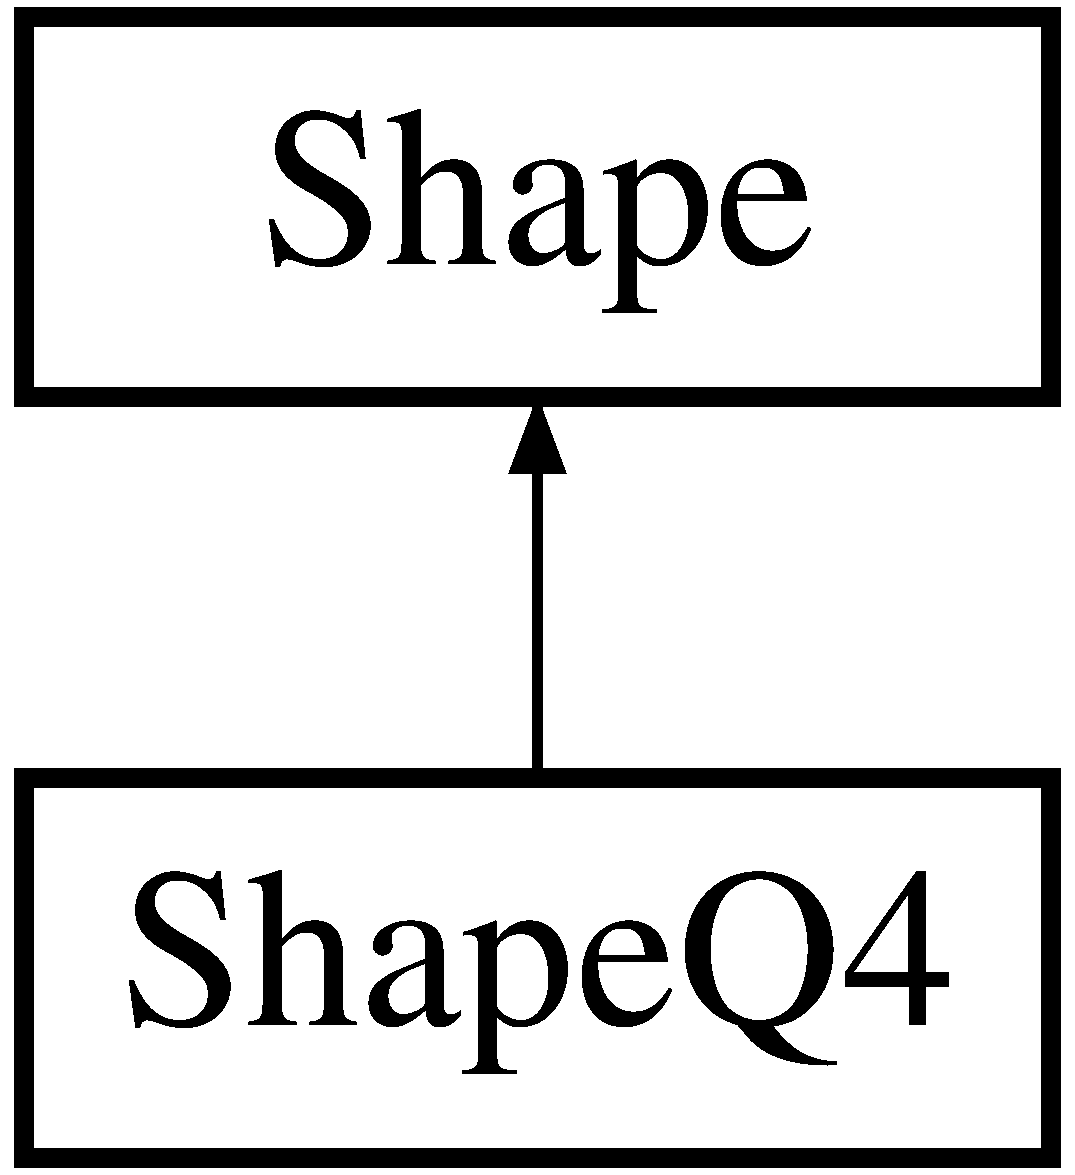
\includegraphics[height=2.000000cm]{class_shape_q4}
\end{center}
\end{figure}
\subsection*{Public Member Functions}
\begin{DoxyCompactItemize}
\item 
Matrix\+Xd \mbox{\hyperlink{class_shape_q4_a306cacfd4d87384b3d06c2788cafd4ba}{function}} (const Vector2d \&point) const
\begin{DoxyCompactList}\small\item\em Stack and interleave the shape Function N above into a matrix for the convenience of stiffness matrix computation. \end{DoxyCompactList}\item 
Matrix\+Xd \mbox{\hyperlink{class_shape_q4_ad3e1f5e25aee96cd21b1c8770c35afd0}{local\+Deriv}} (const Vector2d \&point) const
\begin{DoxyCompactList}\small\item\em Compute the local derivatives d\+N/d(xi) and d\+N/d(eta) of the shape function at a given point in isoparametric coordinates. \end{DoxyCompactList}\item 
const std\+::vector$<$ Vector2d $>$ \& \mbox{\hyperlink{class_shape_q4_a5c185036352eabf489007b92f6d48ad2}{gaussian\+Point}} () const
\begin{DoxyCompactList}\small\item\em Get the gaussian integration points to be used in load distribution and stress/strain computation. \end{DoxyCompactList}\item 
const std\+::vector$<$ double $>$ \& \mbox{\hyperlink{class_shape_q4_a51233dd1caaabbe8404c06b5b0db5755}{gaussian\+Weight}} () const
\begin{DoxyCompactList}\small\item\em Get the gaussian integration weights to be used in load distribution and stress/strain computation. \end{DoxyCompactList}\end{DoxyCompactItemize}


\subsection{Member Function Documentation}
\mbox{\Hypertarget{class_shape_q4_a306cacfd4d87384b3d06c2788cafd4ba}\label{class_shape_q4_a306cacfd4d87384b3d06c2788cafd4ba}} 
\index{Shape\+Q4@{Shape\+Q4}!function@{function}}
\index{function@{function}!Shape\+Q4@{Shape\+Q4}}
\subsubsection{\texorpdfstring{function()}{function()}}
{\footnotesize\ttfamily Matrix\+Xd Shape\+Q4\+::function (\begin{DoxyParamCaption}\item[{const Vector2d \&}]{point }\end{DoxyParamCaption}) const\hspace{0.3cm}{\ttfamily [virtual]}}



Stack and interleave the shape Function N above into a matrix for the convenience of stiffness matrix computation. 

If n is the number of nodes of this element type, then this function will returns a 2-\/by-\/2n matrix\+:

\mbox{[} N1(x) 0 $\vert$ N2(x) 0 $\vert$ ... $\vert$ Nn(x) 0 \mbox{]} \mbox{[} 0 N1(x) $\vert$ 0 N2(x) $\vert$ ... $\vert$ 0 Nn(x) \mbox{]}

this is because our displacement vector is stored in an interleaving form as \mbox{[}r1, z1, r2, z2, ..., rn, zn\mbox{]}.


\begin{DoxyParams}{Parameters}
{\em point} & A 2D point x(r,z) at which the shape function to be evaluated. Pass-\/by-\/ref. \\
\hline
\end{DoxyParams}
\begin{DoxyReturn}{Returns}
The stacked and interleaved shape function N as a matrix at given point. 
\end{DoxyReturn}


Implements \mbox{\hyperlink{class_shape_ab6e0d64b40e09c176ce2ece24bc94a37}{Shape}}.

\mbox{\Hypertarget{class_shape_q4_a5c185036352eabf489007b92f6d48ad2}\label{class_shape_q4_a5c185036352eabf489007b92f6d48ad2}} 
\index{Shape\+Q4@{Shape\+Q4}!gaussian\+Point@{gaussian\+Point}}
\index{gaussian\+Point@{gaussian\+Point}!Shape\+Q4@{Shape\+Q4}}
\subsubsection{\texorpdfstring{gaussian\+Point()}{gaussianPoint()}}
{\footnotesize\ttfamily const std\+::vector$<$ Vector2d $>$ \& Shape\+Q4\+::gaussian\+Point (\begin{DoxyParamCaption}{ }\end{DoxyParamCaption}) const\hspace{0.3cm}{\ttfamily [virtual]}}



Get the gaussian integration points to be used in load distribution and stress/strain computation. 

\begin{DoxyReturn}{Returns}
An array of 2D points. Since the whole \mbox{\hyperlink{class_shape}{Shape}} object is dynamically allocated on heap, we can return-\/by-\/ref. 
\end{DoxyReturn}


Implements \mbox{\hyperlink{class_shape_afa8029d0991fc5d9054a667823224bd0}{Shape}}.

\mbox{\Hypertarget{class_shape_q4_a51233dd1caaabbe8404c06b5b0db5755}\label{class_shape_q4_a51233dd1caaabbe8404c06b5b0db5755}} 
\index{Shape\+Q4@{Shape\+Q4}!gaussian\+Weight@{gaussian\+Weight}}
\index{gaussian\+Weight@{gaussian\+Weight}!Shape\+Q4@{Shape\+Q4}}
\subsubsection{\texorpdfstring{gaussian\+Weight()}{gaussianWeight()}}
{\footnotesize\ttfamily const std\+::vector$<$ double $>$ \& Shape\+Q4\+::gaussian\+Weight (\begin{DoxyParamCaption}{ }\end{DoxyParamCaption}) const\hspace{0.3cm}{\ttfamily [virtual]}}



Get the gaussian integration weights to be used in load distribution and stress/strain computation. 

\begin{DoxyReturn}{Returns}
An array of weight values. Since the whole \mbox{\hyperlink{class_shape}{Shape}} object is dynamically allocated on heap, we can return-\/by-\/ref. 
\end{DoxyReturn}


Implements \mbox{\hyperlink{class_shape_a4257697bb443af2871a7cc7a82c8c823}{Shape}}.

\mbox{\Hypertarget{class_shape_q4_ad3e1f5e25aee96cd21b1c8770c35afd0}\label{class_shape_q4_ad3e1f5e25aee96cd21b1c8770c35afd0}} 
\index{Shape\+Q4@{Shape\+Q4}!local\+Deriv@{local\+Deriv}}
\index{local\+Deriv@{local\+Deriv}!Shape\+Q4@{Shape\+Q4}}
\subsubsection{\texorpdfstring{local\+Deriv()}{localDeriv()}}
{\footnotesize\ttfamily Matrix\+Xd Shape\+Q4\+::local\+Deriv (\begin{DoxyParamCaption}\item[{const Vector2d \&}]{point }\end{DoxyParamCaption}) const\hspace{0.3cm}{\ttfamily [virtual]}}



Compute the local derivatives d\+N/d(xi) and d\+N/d(eta) of the shape function at a given point in isoparametric coordinates. 

If n is the number of nodes of this element type, then this function will returns a 2-\/by-\/n matrix\+:

\mbox{[} d\+N1(x)/d(xi) d\+N2(x)/d(xi) ... d\+Nn(x)/d(xi) \mbox{]} \mbox{[} d\+N1(x)/d(eta) d\+N2(x)/d(eta) ... d\+Nn(x)/d(eta) \mbox{]}


\begin{DoxyParams}{Parameters}
{\em point} & A 2D point x(r,z) at which the shape function to be evaluated. Pass-\/by-\/ref. \\
\hline
\end{DoxyParams}
\begin{DoxyReturn}{Returns}
The stacked and interleaved shape function N as a matrix at given point. 
\end{DoxyReturn}


Implements \mbox{\hyperlink{class_shape_a55575394f656e3ee4b5ac37ea04af8c9}{Shape}}.



The documentation for this class was generated from the following files\+:\begin{DoxyCompactItemize}
\item 
\mbox{\hyperlink{_shape_q4_8h}{Shape\+Q4.\+h}}\item 
\mbox{\hyperlink{_shape_q4_8cpp}{Shape\+Q4.\+cpp}}\end{DoxyCompactItemize}

\hypertarget{class_shape_q8}{}\section{Shape\+Q8 Class Reference}
\label{class_shape_q8}\index{Shape\+Q8@{Shape\+Q8}}
Inheritance diagram for Shape\+Q8\+:\begin{figure}[H]
\begin{center}
\leavevmode
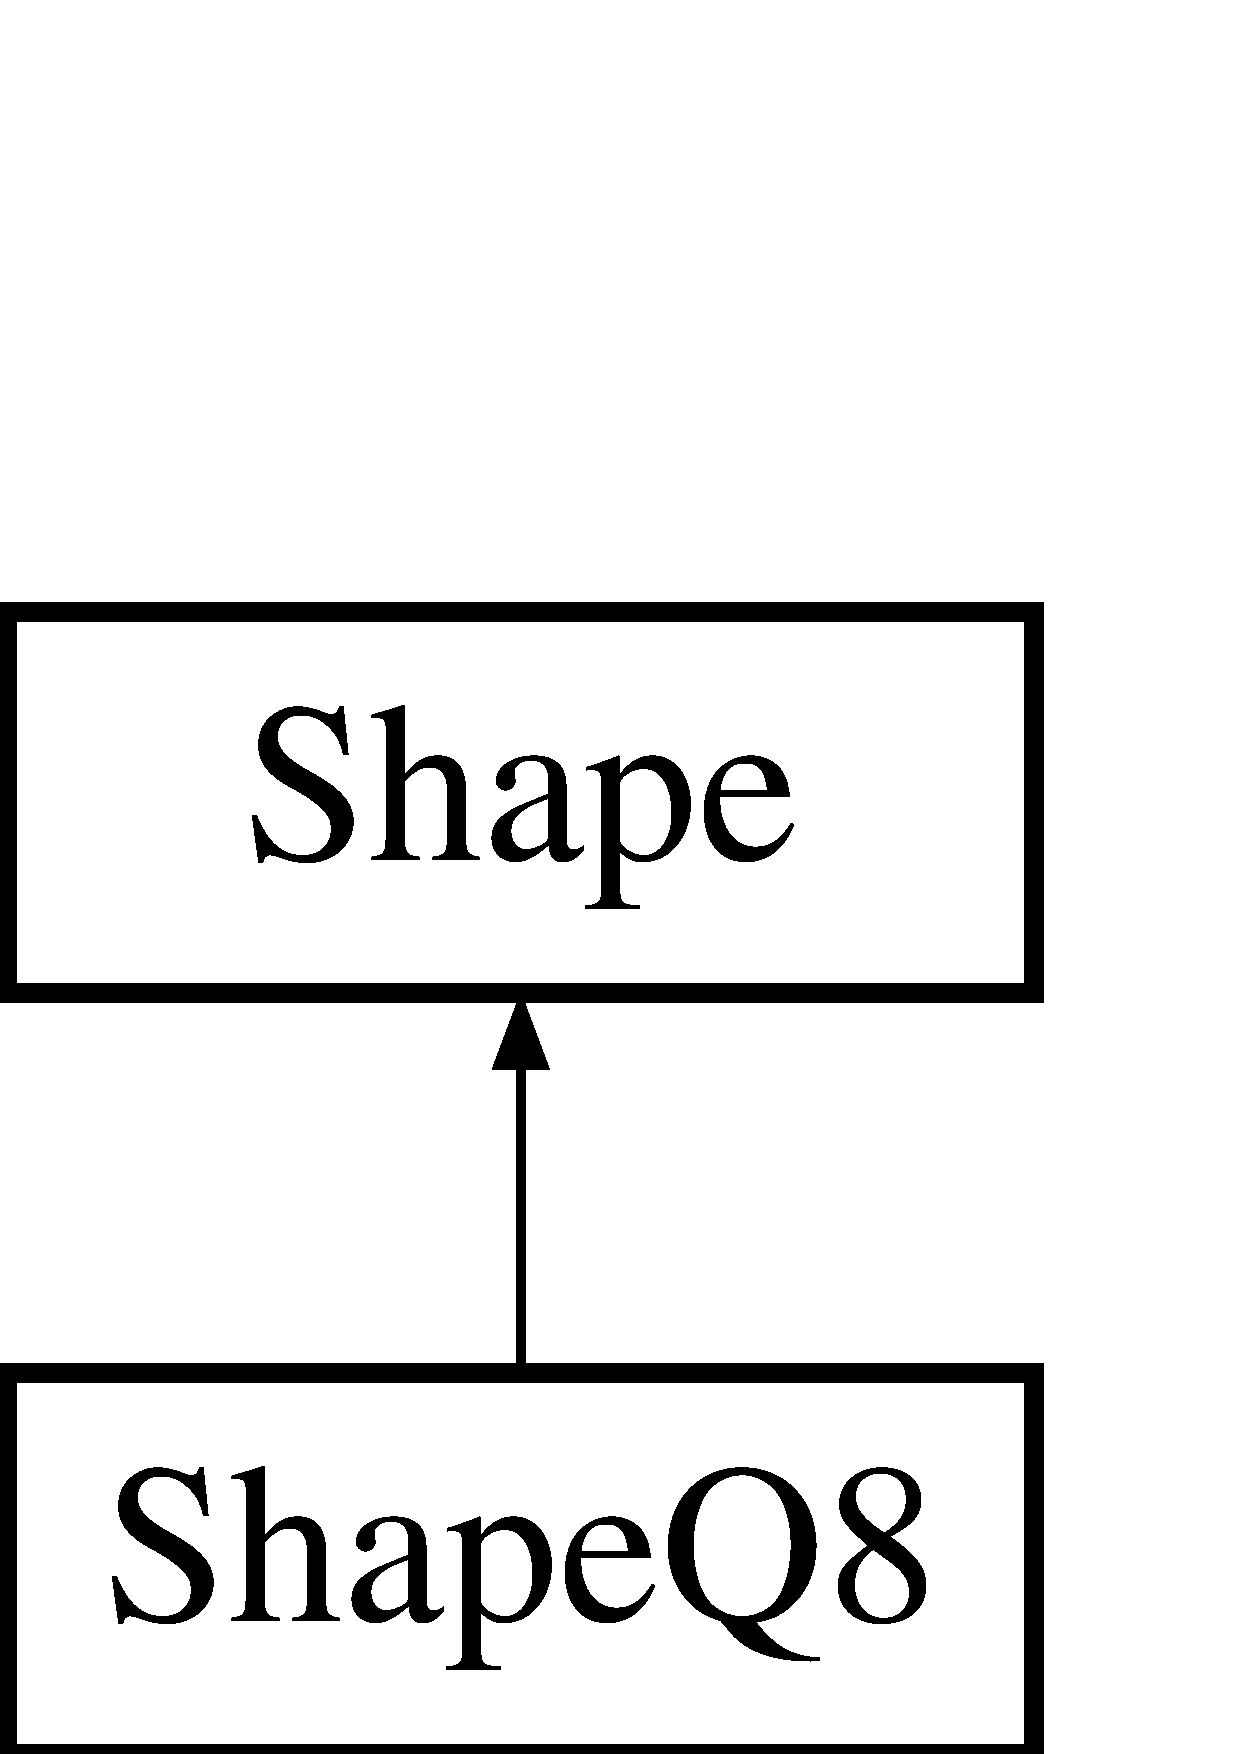
\includegraphics[height=2.000000cm]{class_shape_q8}
\end{center}
\end{figure}
\subsection*{Public Member Functions}
\begin{DoxyCompactItemize}
\item 
Vector\+Xd \mbox{\hyperlink{class_shape_q8_a7e2de42658deff3c6912cc102b12cc96}{function\+Vec}} (const Vector2d \&point) const
\begin{DoxyCompactList}\small\item\em Compute the shape Function N in a column vector at a given point. \end{DoxyCompactList}\item 
Matrix\+Xd \mbox{\hyperlink{class_shape_q8_a7e859a85ee52c8d3ab3051326fc09ab0}{function}} (const Vector2d \&point) const
\begin{DoxyCompactList}\small\item\em Stack and interleave the shape Function N above into a matrix for the convenience of stiffness matrix computation. \end{DoxyCompactList}\item 
Matrix\+Xd \mbox{\hyperlink{class_shape_q8_ac62182e6804216500c2b290efd5fd06a}{local\+Deriv}} (const Vector2d \&point) const
\begin{DoxyCompactList}\small\item\em Compute the local derivatives d\+N/d(xi) and d\+N/d(eta) of the shape function at a given point in isoparametric coordinates. \end{DoxyCompactList}\item 
const std\+::vector$<$ Vector2d $>$ \& \mbox{\hyperlink{class_shape_q8_a197f1e2109c7ee6c29d27198c96928a4}{gaussian\+Point}} () const
\begin{DoxyCompactList}\small\item\em Get the gaussian integration points to be used in load distribution and stress/strain computation. \end{DoxyCompactList}\item 
const std\+::vector$<$ double $>$ \& \mbox{\hyperlink{class_shape_q8_a30891417d7ba6d6457b8b5567add07f5}{gaussian\+Weight}} () const
\begin{DoxyCompactList}\small\item\em Get the gaussian integration weights to be used in load distribution and stress/strain computation. \end{DoxyCompactList}\end{DoxyCompactItemize}


\subsection{Member Function Documentation}
\mbox{\Hypertarget{class_shape_q8_a7e859a85ee52c8d3ab3051326fc09ab0}\label{class_shape_q8_a7e859a85ee52c8d3ab3051326fc09ab0}} 
\index{Shape\+Q8@{Shape\+Q8}!function@{function}}
\index{function@{function}!Shape\+Q8@{Shape\+Q8}}
\subsubsection{\texorpdfstring{function()}{function()}}
{\footnotesize\ttfamily Matrix\+Xd Shape\+Q8\+::function (\begin{DoxyParamCaption}\item[{const Vector2d \&}]{point }\end{DoxyParamCaption}) const\hspace{0.3cm}{\ttfamily [virtual]}}



Stack and interleave the shape Function N above into a matrix for the convenience of stiffness matrix computation. 

If n is the number of nodes of this element type, then this function will returns a 2-\/by-\/2n matrix\+:

\mbox{[} N1(x) 0 $\vert$ N2(x) 0 $\vert$ ... $\vert$ Nn(x) 0 \mbox{]} \mbox{[} 0 N1(x) $\vert$ 0 N2(x) $\vert$ ... $\vert$ 0 Nn(x) \mbox{]}

this is because our displacement vector is stored in an interleaving form as \mbox{[}r1, z1, r2, z2, ..., rn, zn\mbox{]}.


\begin{DoxyParams}{Parameters}
{\em point} & A 2D point x(r,z) at which the shape function to be evaluated. Pass-\/by-\/ref. \\
\hline
\end{DoxyParams}
\begin{DoxyReturn}{Returns}
The stacked and interleaved shape function N as a matrix at given point. 
\end{DoxyReturn}


Implements \mbox{\hyperlink{class_shape_ab6e0d64b40e09c176ce2ece24bc94a37}{Shape}}.

\mbox{\Hypertarget{class_shape_q8_a7e2de42658deff3c6912cc102b12cc96}\label{class_shape_q8_a7e2de42658deff3c6912cc102b12cc96}} 
\index{Shape\+Q8@{Shape\+Q8}!function\+Vec@{function\+Vec}}
\index{function\+Vec@{function\+Vec}!Shape\+Q8@{Shape\+Q8}}
\subsubsection{\texorpdfstring{function\+Vec()}{functionVec()}}
{\footnotesize\ttfamily Vector\+Xd Shape\+Q8\+::function\+Vec (\begin{DoxyParamCaption}\item[{const Vector2d \&}]{point }\end{DoxyParamCaption}) const\hspace{0.3cm}{\ttfamily [virtual]}}



Compute the shape Function N in a column vector at a given point. 

If n is the number of nodes of this element type, then this function will returns a n-\/by-\/1 column vector\+:

\mbox{[} N1(x), N2(x), ..., Nn(x) \mbox{]}

where Ni(x) is the shape function with respect to ith node at point x.


\begin{DoxyParams}{Parameters}
{\em point} & A 2D point x(r,z) at which the shape function to be evaluated. Pass-\/by-\/ref. \\
\hline
\end{DoxyParams}
\begin{DoxyReturn}{Returns}
The shape function N as a column vector at given point.
\end{DoxyReturn}
\begin{DoxyNote}{Note}
Use a const qualifier for reference variable is the recommended programming style. \mbox{\hyperlink{class_shape}{Shape}} function depends on given point, so we can only return-\/by-\/value, no more space for optimization. 
\end{DoxyNote}


Implements \mbox{\hyperlink{class_shape_a0e0400bca54c29b5097c84ace51ecc7b}{Shape}}.

\mbox{\Hypertarget{class_shape_q8_a197f1e2109c7ee6c29d27198c96928a4}\label{class_shape_q8_a197f1e2109c7ee6c29d27198c96928a4}} 
\index{Shape\+Q8@{Shape\+Q8}!gaussian\+Point@{gaussian\+Point}}
\index{gaussian\+Point@{gaussian\+Point}!Shape\+Q8@{Shape\+Q8}}
\subsubsection{\texorpdfstring{gaussian\+Point()}{gaussianPoint()}}
{\footnotesize\ttfamily const std\+::vector$<$ Vector2d $>$ \& Shape\+Q8\+::gaussian\+Point (\begin{DoxyParamCaption}{ }\end{DoxyParamCaption}) const\hspace{0.3cm}{\ttfamily [virtual]}}



Get the gaussian integration points to be used in load distribution and stress/strain computation. 

\begin{DoxyReturn}{Returns}
An array of 2D points. Since the whole \mbox{\hyperlink{class_shape}{Shape}} object is dynamically allocated on heap, we can return-\/by-\/ref. 
\end{DoxyReturn}


Implements \mbox{\hyperlink{class_shape_afa8029d0991fc5d9054a667823224bd0}{Shape}}.

\mbox{\Hypertarget{class_shape_q8_a30891417d7ba6d6457b8b5567add07f5}\label{class_shape_q8_a30891417d7ba6d6457b8b5567add07f5}} 
\index{Shape\+Q8@{Shape\+Q8}!gaussian\+Weight@{gaussian\+Weight}}
\index{gaussian\+Weight@{gaussian\+Weight}!Shape\+Q8@{Shape\+Q8}}
\subsubsection{\texorpdfstring{gaussian\+Weight()}{gaussianWeight()}}
{\footnotesize\ttfamily const std\+::vector$<$ double $>$ \& Shape\+Q8\+::gaussian\+Weight (\begin{DoxyParamCaption}{ }\end{DoxyParamCaption}) const\hspace{0.3cm}{\ttfamily [virtual]}}



Get the gaussian integration weights to be used in load distribution and stress/strain computation. 

\begin{DoxyReturn}{Returns}
An array of weight values. Since the whole \mbox{\hyperlink{class_shape}{Shape}} object is dynamically allocated on heap, we can return-\/by-\/ref. 
\end{DoxyReturn}


Implements \mbox{\hyperlink{class_shape_a4257697bb443af2871a7cc7a82c8c823}{Shape}}.

\mbox{\Hypertarget{class_shape_q8_ac62182e6804216500c2b290efd5fd06a}\label{class_shape_q8_ac62182e6804216500c2b290efd5fd06a}} 
\index{Shape\+Q8@{Shape\+Q8}!local\+Deriv@{local\+Deriv}}
\index{local\+Deriv@{local\+Deriv}!Shape\+Q8@{Shape\+Q8}}
\subsubsection{\texorpdfstring{local\+Deriv()}{localDeriv()}}
{\footnotesize\ttfamily Matrix\+Xd Shape\+Q8\+::local\+Deriv (\begin{DoxyParamCaption}\item[{const Vector2d \&}]{point }\end{DoxyParamCaption}) const\hspace{0.3cm}{\ttfamily [virtual]}}



Compute the local derivatives d\+N/d(xi) and d\+N/d(eta) of the shape function at a given point in isoparametric coordinates. 

If n is the number of nodes of this element type, then this function will returns a 2-\/by-\/n matrix\+:

\mbox{[} d\+N1(x)/d(xi) d\+N2(x)/d(xi) ... d\+Nn(x)/d(xi) \mbox{]} \mbox{[} d\+N1(x)/d(eta) d\+N2(x)/d(eta) ... d\+Nn(x)/d(eta) \mbox{]}


\begin{DoxyParams}{Parameters}
{\em point} & A 2D point x(r,z) at which the shape function to be evaluated. Pass-\/by-\/ref. \\
\hline
\end{DoxyParams}
\begin{DoxyReturn}{Returns}
The stacked and interleaved shape function N as a matrix at given point. 
\end{DoxyReturn}


Implements \mbox{\hyperlink{class_shape_a55575394f656e3ee4b5ac37ea04af8c9}{Shape}}.



The documentation for this class was generated from the following files\+:\begin{DoxyCompactItemize}
\item 
\mbox{\hyperlink{_shape_q8_8h}{Shape\+Q8.\+h}}\item 
\mbox{\hyperlink{_shape_q8_8cpp}{Shape\+Q8.\+cpp}}\end{DoxyCompactItemize}

\hypertarget{struct_element_1_1static_members}{}\section{Element\+:\+:static\+Members Struct Reference}
\label{struct_element_1_1static_members}\index{Element\+::static\+Members@{Element\+::static\+Members}}
\subsection*{Public Member Functions}
\begin{DoxyCompactItemize}
\item 
\mbox{\hyperlink{struct_element_1_1static_members_a1686a16e7655673413d850e7ab8d0aea}{static\+Members}} (int nodes, int gaussians, int edges, int edge\+Nodes, int edge\+Gaussians)
\begin{DoxyCompactList}\small\item\em Constructor for the strucuture. \end{DoxyCompactList}\item 
\mbox{\Hypertarget{struct_element_1_1static_members_afc6b24b9e09467da8f832c44e3aa9d1c}\label{struct_element_1_1static_members_afc6b24b9e09467da8f832c44e3aa9d1c}} 
\mbox{\hyperlink{struct_element_1_1static_members_afc6b24b9e09467da8f832c44e3aa9d1c}{$\sim$static\+Members}} ()
\begin{DoxyCompactList}\small\item\em Destructor for the strucuture. \end{DoxyCompactList}\end{DoxyCompactItemize}
\subsection*{Public Attributes}
\begin{DoxyCompactItemize}
\item 
\mbox{\hyperlink{class_shape}{Shape}} $\ast$ \mbox{\hyperlink{struct_element_1_1static_members_ae4cc99299c3d19da297d8faec65529c6}{shape}}
\begin{DoxyCompactList}\small\item\em A pointer to the shape instance of this element type. \end{DoxyCompactList}\end{DoxyCompactItemize}


\subsection{Constructor \& Destructor Documentation}
\mbox{\Hypertarget{struct_element_1_1static_members_a1686a16e7655673413d850e7ab8d0aea}\label{struct_element_1_1static_members_a1686a16e7655673413d850e7ab8d0aea}} 
\index{Element\+::static\+Members@{Element\+::static\+Members}!static\+Members@{static\+Members}}
\index{static\+Members@{static\+Members}!Element\+::static\+Members@{Element\+::static\+Members}}
\subsubsection{\texorpdfstring{static\+Members()}{staticMembers()}}
{\footnotesize\ttfamily Element\+::static\+Members\+::static\+Members (\begin{DoxyParamCaption}\item[{int}]{nodes,  }\item[{int}]{gaussians,  }\item[{int}]{edges,  }\item[{int}]{edge\+Nodes,  }\item[{int}]{edge\+Gaussians }\end{DoxyParamCaption})\hspace{0.3cm}{\ttfamily [inline]}}



Constructor for the strucuture. 


\begin{DoxyParams}{Parameters}
{\em nodes} & Number of nodes of this shape of element. \\
\hline
{\em gaussians} & Number of Gaussian integration points of this shape of element. \\
\hline
{\em edges} & Number of edges of this shape of element. \\
\hline
{\em edge\+Nodes} & Number of nodes each edge consists of. \\
\hline
{\em edge\+Gaussians} & Number of Gaussian intergration points at each edge. \\
\hline
\end{DoxyParams}


\subsection{Member Data Documentation}
\mbox{\Hypertarget{struct_element_1_1static_members_ae4cc99299c3d19da297d8faec65529c6}\label{struct_element_1_1static_members_ae4cc99299c3d19da297d8faec65529c6}} 
\index{Element\+::static\+Members@{Element\+::static\+Members}!shape@{shape}}
\index{shape@{shape}!Element\+::static\+Members@{Element\+::static\+Members}}
\subsubsection{\texorpdfstring{shape}{shape}}
{\footnotesize\ttfamily \mbox{\hyperlink{class_shape}{Shape}}$\ast$ Element\+::static\+Members\+::shape}



A pointer to the shape instance of this element type. 



The documentation for this struct was generated from the following file\+:\begin{DoxyCompactItemize}
\item 
\mbox{\hyperlink{_element_8h}{Element.\+h}}\end{DoxyCompactItemize}

\chapter{File Documentation}
\hypertarget{_analysis_8cpp}{}\section{Analysis.\+cpp File Reference}
\label{_analysis_8cpp}\index{Analysis.\+cpp@{Analysis.\+cpp}}


Implementation of \mbox{\hyperlink{class_analysis}{Analysis}} class.  


{\ttfamily \#include $<$cmath$>$}\newline
{\ttfamily \#include \char`\"{}Analysis.\+h\char`\"{}}\newline
{\ttfamily \#include $<$iostream$>$}\newline
{\ttfamily \#include $<$fstream$>$}\newline
{\ttfamily \#include $<$iomanip$>$}\newline
{\ttfamily \#include $<$unordered\+\_\+map$>$}\newline


\subsection{Detailed Description}
Implementation of \mbox{\hyperlink{class_analysis}{Analysis}} class. 

\begin{DoxyAuthor}{Author}
Haohang Huang 
\end{DoxyAuthor}
\begin{DoxyDate}{Date}
Feburary 26, 2018 
\end{DoxyDate}

\hypertarget{_analysis_8h}{}\section{Analysis.\+h File Reference}
\label{_analysis_8h}\index{Analysis.\+h@{Analysis.\+h}}


Abstract \mbox{\hyperlink{class_analysis}{Analysis}} class for various types of analysis.  


{\ttfamily \#include \char`\"{}Mesh.\+h\char`\"{}}\newline
\subsection*{Classes}
\begin{DoxyCompactItemize}
\item 
class \mbox{\hyperlink{class_analysis}{Analysis}}
\end{DoxyCompactItemize}


\subsection{Detailed Description}
Abstract \mbox{\hyperlink{class_analysis}{Analysis}} class for various types of analysis. 

\begin{DoxyAuthor}{Author}
Haohang Huang 
\end{DoxyAuthor}
\begin{DoxyDate}{Date}
Feburary 26, 2018 
\end{DoxyDate}
\begin{DoxyNote}{Note}
No efficiency optimization required on March 26, 2018.  Query point method. 
\end{DoxyNote}

\hypertarget{_element_8cpp}{}\section{Element.\+cpp File Reference}
\label{_element_8cpp}\index{Element.\+cpp@{Element.\+cpp}}


Implementation of \mbox{\hyperlink{class_element}{Element}} class.  


{\ttfamily \#include $<$cmath$>$}\newline
{\ttfamily \#include \char`\"{}Element.\+h\char`\"{}}\newline


\subsection{Detailed Description}
Implementation of \mbox{\hyperlink{class_element}{Element}} class. 

\begin{DoxyAuthor}{Author}
Haohang Huang 
\end{DoxyAuthor}
\begin{DoxyDate}{Date}
Feburary 4, 2018 
\end{DoxyDate}

\hypertarget{_element_8h}{}\section{Element.\+h File Reference}
\label{_element_8h}\index{Element.\+h@{Element.\+h}}


Abstract base class for various isoparametric elements.  


{\ttfamily \#include \char`\"{}Node.\+h\char`\"{}}\newline
{\ttfamily \#include \char`\"{}Shape.\+h\char`\"{}}\newline
\subsection*{Classes}
\begin{DoxyCompactItemize}
\item 
class \mbox{\hyperlink{class_element}{Element}}
\end{DoxyCompactItemize}


\subsection{Detailed Description}
Abstract base class for various isoparametric elements. 

\begin{DoxyAuthor}{Author}
Haohang Huang 
\end{DoxyAuthor}
\begin{DoxyDate}{Date}
Feburary 4, 2018 
\end{DoxyDate}
\begin{DoxyNote}{Note}
Efficiency optimized by return-\/by-\/ref on March 26, 2018. 
\end{DoxyNote}

\hypertarget{_element_q4_8cpp}{}\section{Element\+Q4.\+cpp File Reference}
\label{_element_q4_8cpp}\index{Element\+Q4.\+cpp@{Element\+Q4.\+cpp}}


Implementation of \mbox{\hyperlink{class_element_q4}{Element\+Q4}} class.  


{\ttfamily \#include \char`\"{}Element\+Q4.\+h\char`\"{}}\newline


\subsection{Detailed Description}
Implementation of \mbox{\hyperlink{class_element_q4}{Element\+Q4}} class. 

\begin{DoxyAuthor}{Author}
Haohang Huang 
\end{DoxyAuthor}
\begin{DoxyDate}{Date}
Feburary 10, 2018 
\end{DoxyDate}

\hypertarget{_element_q4_8h}{}\section{Element\+Q4.\+h File Reference}
\label{_element_q4_8h}\index{Element\+Q4.\+h@{Element\+Q4.\+h}}


Derived class from \mbox{\hyperlink{class_element}{Element}} for the isoparametric Q4 element.  


{\ttfamily \#include \char`\"{}Element.\+h\char`\"{}}\newline
{\ttfamily \#include \char`\"{}Shape\+Q4.\+h\char`\"{}}\newline
\subsection*{Classes}
\begin{DoxyCompactItemize}
\item 
class \mbox{\hyperlink{class_element_q4}{Element\+Q4}}
\end{DoxyCompactItemize}


\subsection{Detailed Description}
Derived class from \mbox{\hyperlink{class_element}{Element}} for the isoparametric Q4 element. 

\begin{DoxyAuthor}{Author}
Haohang Huang 
\end{DoxyAuthor}
\begin{DoxyDate}{Date}
Feburary 10, 2018 
\end{DoxyDate}

\hypertarget{_element_q8_8cpp}{}\section{Element\+Q8.\+cpp File Reference}
\label{_element_q8_8cpp}\index{Element\+Q8.\+cpp@{Element\+Q8.\+cpp}}


Implementation of \mbox{\hyperlink{class_element_q8}{Element\+Q8}} class.  


{\ttfamily \#include \char`\"{}Element\+Q8.\+h\char`\"{}}\newline
{\ttfamily \#include $<$cmath$>$}\newline


\subsection{Detailed Description}
Implementation of \mbox{\hyperlink{class_element_q8}{Element\+Q8}} class. 

\begin{DoxyAuthor}{Author}
Haohang Huang 
\end{DoxyAuthor}
\begin{DoxyDate}{Date}
Feburary 13, 2018 
\end{DoxyDate}

\hypertarget{_element_q8_8h}{}\section{Element\+Q8.\+h File Reference}
\label{_element_q8_8h}\index{Element\+Q8.\+h@{Element\+Q8.\+h}}


Derived class from \mbox{\hyperlink{class_element}{Element}} for the isoparametric Q8 element.  


{\ttfamily \#include \char`\"{}Element.\+h\char`\"{}}\newline
\subsection*{Classes}
\begin{DoxyCompactItemize}
\item 
class \mbox{\hyperlink{class_element_q8}{Element\+Q8}}
\end{DoxyCompactItemize}


\subsection{Detailed Description}
Derived class from \mbox{\hyperlink{class_element}{Element}} for the isoparametric Q8 element. 

\begin{DoxyAuthor}{Author}
Haohang Huang 
\end{DoxyAuthor}
\begin{DoxyDate}{Date}
Feburary 13, 2018 
\end{DoxyDate}
\begin{DoxyNote}{Note}
Efficiency optimized by polymorph shape on March 26, 2018. 

Efficiency optimized by storing local stiffness matrix and return-\/by-\/ref on March 27, 2018 

Efficiency optimized by the generalization of all element-\/wise operations into base class \mbox{\hyperlink{class_element}{Element}} on Apr 22, 2018. 
\end{DoxyNote}

\hypertarget{_element_t6_8cpp}{}\section{Element\+T6.\+cpp File Reference}
\label{_element_t6_8cpp}\index{Element\+T6.\+cpp@{Element\+T6.\+cpp}}


Implementation of Element\+T6 class.  




\subsection{Detailed Description}
Implementation of Element\+T6 class. 

\begin{DoxyAuthor}{Author}
Haohang Huang 
\end{DoxyAuthor}
\begin{DoxyDate}{Date}
Apr 22, 2018 
\end{DoxyDate}

\hypertarget{_element_t6_8h}{}\section{Element\+T6.\+h File Reference}
\label{_element_t6_8h}\index{Element\+T6.\+h@{Element\+T6.\+h}}


Derived class from \mbox{\hyperlink{class_element}{Element}} for the isoparametric T6 element.  




\subsection{Detailed Description}
Derived class from \mbox{\hyperlink{class_element}{Element}} for the isoparametric T6 element. 

\begin{DoxyAuthor}{Author}
Haohang Huang 
\end{DoxyAuthor}
\begin{DoxyDate}{Date}
Apr 22, 2018 
\end{DoxyDate}

\hypertarget{_linear_elastic_8cpp}{}\section{Linear\+Elastic.\+cpp File Reference}
\label{_linear_elastic_8cpp}\index{Linear\+Elastic.\+cpp@{Linear\+Elastic.\+cpp}}


Implementation of \mbox{\hyperlink{class_linear_elastic}{Linear\+Elastic}} class.  


{\ttfamily \#include \char`\"{}Linear\+Elastic.\+h\char`\"{}}\newline
{\ttfamily \#include $<$chrono$>$}\newline
{\ttfamily \#include $<$iostream$>$}\newline


\subsection{Detailed Description}
Implementation of \mbox{\hyperlink{class_linear_elastic}{Linear\+Elastic}} class. 

\begin{DoxyAuthor}{Author}
Haohang Huang 
\end{DoxyAuthor}
\begin{DoxyDate}{Date}
Feburary 26, 2018 
\end{DoxyDate}

\hypertarget{_linear_elastic_8h}{}\section{Linear\+Elastic.\+h File Reference}
\label{_linear_elastic_8h}\index{Linear\+Elastic.\+h@{Linear\+Elastic.\+h}}


Derived class from \mbox{\hyperlink{class_analysis}{Analysis}} for linear elastic problems.  


{\ttfamily \#include \char`\"{}Analysis.\+h\char`\"{}}\newline
\subsection*{Classes}
\begin{DoxyCompactItemize}
\item 
class \mbox{\hyperlink{class_linear_elastic}{Linear\+Elastic}}
\end{DoxyCompactItemize}


\subsection{Detailed Description}
Derived class from \mbox{\hyperlink{class_analysis}{Analysis}} for linear elastic problems. 

\begin{DoxyAuthor}{Author}
Haohang Huang 
\end{DoxyAuthor}
\begin{DoxyDate}{Date}
Feburary 26, 2018 
\end{DoxyDate}
\begin{DoxyNote}{Note}
No efficiency optimization required on March 26, 2018. 
\end{DoxyNote}

\hypertarget{main_8cpp}{}\section{main.\+cpp File Reference}
\label{main_8cpp}\index{main.\+cpp@{main.\+cpp}}


Main execution interface.  


{\ttfamily \#include $<$iostream$>$}\newline
{\ttfamily \#include $<$fstream$>$}\newline
{\ttfamily \#include $<$string$>$}\newline
{\ttfamily \#include $<$chrono$>$}\newline
{\ttfamily \#include \char`\"{}Linear\+Elastic.\+h\char`\"{}}\newline
{\ttfamily \#include \char`\"{}I\+O.\+h\char`\"{}}\newline
\subsection*{Functions}
\begin{DoxyCompactItemize}
\item 
\mbox{\Hypertarget{main_8cpp_ae66f6b31b5ad750f1fe042a706a4e3d4}\label{main_8cpp_ae66f6b31b5ad750f1fe042a706a4e3d4}} 
int {\bfseries main} ()
\end{DoxyCompactItemize}


\subsection{Detailed Description}
Main execution interface. 

\begin{DoxyAuthor}{Author}
Haohang Huang 
\end{DoxyAuthor}
\begin{DoxyDate}{Date}
Feburary 4, 2018 
\end{DoxyDate}

\hypertarget{_material_8cpp}{}\section{Material.\+cpp File Reference}
\label{_material_8cpp}\index{Material.\+cpp@{Material.\+cpp}}


Implementation of the \mbox{\hyperlink{class_material}{Material}} class.  


{\ttfamily \#include \char`\"{}Material.\+h\char`\"{}}\newline


\subsection{Detailed Description}
Implementation of the \mbox{\hyperlink{class_material}{Material}} class. 

\begin{DoxyAuthor}{Author}
Haohang Huang 
\end{DoxyAuthor}
\begin{DoxyDate}{Date}
Apr 27, 2018 
\end{DoxyDate}

\hypertarget{_material_8h}{}\section{Material.\+h File Reference}
\label{_material_8h}\index{Material.\+h@{Material.\+h}}


\mbox{\hyperlink{class_material}{Material}} class for the element properties.  


{\ttfamily \#include \char`\"{}Eigen/\+Eigen\char`\"{}}\newline
{\ttfamily \#include $<$vector$>$}\newline
\subsection*{Classes}
\begin{DoxyCompactItemize}
\item 
class \mbox{\hyperlink{class_material}{Material}}
\begin{DoxyCompactList}\small\item\em \mbox{\hyperlink{class_material}{Material}} class for storing the engineering properties of elements. \end{DoxyCompactList}\end{DoxyCompactItemize}


\subsection{Detailed Description}
\mbox{\hyperlink{class_material}{Material}} class for the element properties. 

\begin{DoxyAuthor}{Author}
Haohang Huang 
\end{DoxyAuthor}
\begin{DoxyDate}{Date}
Apr 27, 2018 
\end{DoxyDate}

\hypertarget{_mesh_8cpp}{}\section{Mesh.\+cpp File Reference}
\label{_mesh_8cpp}\index{Mesh.\+cpp@{Mesh.\+cpp}}


Implementation of \mbox{\hyperlink{class_mesh}{Mesh}} class.  


{\ttfamily \#include \char`\"{}Mesh.\+h\char`\"{}}\newline
{\ttfamily \#include \char`\"{}Element\+Q4.\+h\char`\"{}}\newline
{\ttfamily \#include \char`\"{}Shape\+Q4.\+h\char`\"{}}\newline
{\ttfamily \#include \char`\"{}Element\+Q8.\+h\char`\"{}}\newline
{\ttfamily \#include \char`\"{}Shape\+Q8.\+h\char`\"{}}\newline
{\ttfamily \#include $<$iostream$>$}\newline
{\ttfamily \#include $<$fstream$>$}\newline
{\ttfamily \#include $<$string$>$}\newline
{\ttfamily \#include $<$vector$>$}\newline


\subsection{Detailed Description}
Implementation of \mbox{\hyperlink{class_mesh}{Mesh}} class. 

\begin{DoxyAuthor}{Author}
Haohang Huang 
\end{DoxyAuthor}
\begin{DoxyDate}{Date}
Feburary 5, 2018  line 95, 98, change to T3, Q6 element later  line 124, various load pattern 
\end{DoxyDate}

\hypertarget{_mesh_8h}{}\section{Mesh.\+h File Reference}
\label{_mesh_8h}\index{Mesh.\+h@{Mesh.\+h}}


\mbox{\hyperlink{class_mesh}{Mesh}} class for the entire mesh information read from input file.  


{\ttfamily \#include \char`\"{}Node.\+h\char`\"{}}\newline
{\ttfamily \#include \char`\"{}Element.\+h\char`\"{}}\newline
{\ttfamily \#include $<$vector$>$}\newline
\subsection*{Classes}
\begin{DoxyCompactItemize}
\item 
class \mbox{\hyperlink{class_mesh}{Mesh}}
\end{DoxyCompactItemize}


\subsection{Detailed Description}
\mbox{\hyperlink{class_mesh}{Mesh}} class for the entire mesh information read from input file. 

\begin{DoxyAuthor}{Author}
Haohang Huang 
\end{DoxyAuthor}
\begin{DoxyDate}{Date}
Feburary 5, 2018 
\end{DoxyDate}
\begin{DoxyNote}{Note}
No efficiency optimization required on March 26, 2018 
\end{DoxyNote}

\hypertarget{_node_8cpp}{}\section{Node.\+cpp File Reference}
\label{_node_8cpp}\index{Node.\+cpp@{Node.\+cpp}}


Implementation of \mbox{\hyperlink{class_node}{Node}} class.  


{\ttfamily \#include \char`\"{}Node.\+h\char`\"{}}\newline


\subsection{Detailed Description}
Implementation of \mbox{\hyperlink{class_node}{Node}} class. 

\begin{DoxyAuthor}{Author}
Haohang Huang 
\end{DoxyAuthor}
\begin{DoxyDate}{Date}
Feburary 4, 2018 
\end{DoxyDate}

\hypertarget{_node_8h}{}\section{Node.\+h File Reference}
\label{_node_8h}\index{Node.\+h@{Node.\+h}}


\mbox{\hyperlink{class_node}{Node}} class for the basic coordinates and mechanical properties.  


{\ttfamily \#include \char`\"{}Eigen/\+Eigen\char`\"{}}\newline
\subsection*{Classes}
\begin{DoxyCompactItemize}
\item 
class \mbox{\hyperlink{class_node}{Node}}
\end{DoxyCompactItemize}


\subsection{Detailed Description}
\mbox{\hyperlink{class_node}{Node}} class for the basic coordinates and mechanical properties. 

\begin{DoxyAuthor}{Author}
Haohang Huang 
\end{DoxyAuthor}
\begin{DoxyDate}{Date}
Feburary 4, 2018 
\end{DoxyDate}
\begin{DoxyNote}{Note}
Efficiency optimized by return-\/by-\/ref on March 26, 2018. 
\end{DoxyNote}

\hypertarget{_shape_8cpp}{}\section{Shape.\+cpp File Reference}
\label{_shape_8cpp}\index{Shape.\+cpp@{Shape.\+cpp}}


Implementation of \mbox{\hyperlink{class_shape}{Shape}} class.  


{\ttfamily \#include \char`\"{}Shape.\+h\char`\"{}}\newline
{\ttfamily \#include $<$cmath$>$}\newline


\subsection{Detailed Description}
Implementation of \mbox{\hyperlink{class_shape}{Shape}} class. 

\begin{DoxyAuthor}{Author}
Haohang Huang 
\end{DoxyAuthor}
\begin{DoxyDate}{Date}
Feburary 10, 2018 
\end{DoxyDate}

\hypertarget{_shape_8h}{}\section{Shape.\+h File Reference}
\label{_shape_8h}\index{Shape.\+h@{Shape.\+h}}


Abstract base class for various isoparametric element shapes.  


{\ttfamily \#include \char`\"{}Eigen/\+Eigen\char`\"{}}\newline
{\ttfamily \#include $<$vector$>$}\newline
\subsection*{Classes}
\begin{DoxyCompactItemize}
\item 
class \mbox{\hyperlink{class_shape}{Shape}}
\end{DoxyCompactItemize}


\subsection{Detailed Description}
Abstract base class for various isoparametric element shapes. 

\begin{DoxyAuthor}{Author}
Haohang Huang 
\end{DoxyAuthor}
\begin{DoxyDate}{Date}
Feburary 10, 2018 
\end{DoxyDate}
\begin{DoxyNote}{Note}
Efficiency optimized by return-\/by-\/ref of Gaussian points on March 25, 2018. 
\end{DoxyNote}

\hypertarget{_shape_q4_8cpp}{}\section{Shape\+Q4.\+cpp File Reference}
\label{_shape_q4_8cpp}\index{Shape\+Q4.\+cpp@{Shape\+Q4.\+cpp}}


Implementation of \mbox{\hyperlink{class_shape_q8}{Shape\+Q8}} class.  


{\ttfamily \#include \char`\"{}Shape\+Q4.\+h\char`\"{}}\newline


\subsection{Detailed Description}
Implementation of \mbox{\hyperlink{class_shape_q8}{Shape\+Q8}} class. 

\begin{DoxyAuthor}{Author}
Haohang Huang 
\end{DoxyAuthor}
\begin{DoxyDate}{Date}
Feburary 10, 2018  Gaussian points and function\+Vec not implemented yet. 
\end{DoxyDate}

\hypertarget{_shape_q4_8h}{}\section{Shape\+Q4.\+h File Reference}
\label{_shape_q4_8h}\index{Shape\+Q4.\+h@{Shape\+Q4.\+h}}


Derived class from \mbox{\hyperlink{class_shape}{Shape}} for the shape information of isoparametric Q4 element.  


{\ttfamily \#include \char`\"{}Shape.\+h\char`\"{}}\newline
\subsection*{Classes}
\begin{DoxyCompactItemize}
\item 
class \mbox{\hyperlink{class_shape_q4}{Shape\+Q4}}
\end{DoxyCompactItemize}


\subsection{Detailed Description}
Derived class from \mbox{\hyperlink{class_shape}{Shape}} for the shape information of isoparametric Q4 element. 

\begin{DoxyAuthor}{Author}
Haohang Huang 
\end{DoxyAuthor}
\begin{DoxyDate}{Date}
Feburary 10, 2018  Gaussian points and function\+Vec not implemented yet. 
\end{DoxyDate}

\hypertarget{_shape_q8_8cpp}{}\section{Shape\+Q8.\+cpp File Reference}
\label{_shape_q8_8cpp}\index{Shape\+Q8.\+cpp@{Shape\+Q8.\+cpp}}


Implementation of \mbox{\hyperlink{class_shape_q8}{Shape\+Q8}} class.  


{\ttfamily \#include \char`\"{}Shape\+Q8.\+h\char`\"{}}\newline
{\ttfamily \#include $<$cmath$>$}\newline


\subsection{Detailed Description}
Implementation of \mbox{\hyperlink{class_shape_q8}{Shape\+Q8}} class. 

\begin{DoxyAuthor}{Author}
Haohang Huang 
\end{DoxyAuthor}
\begin{DoxyDate}{Date}
Feburary 13, 2018 
\end{DoxyDate}

\hypertarget{_shape_q8_8h}{}\section{Shape\+Q8.\+h File Reference}
\label{_shape_q8_8h}\index{Shape\+Q8.\+h@{Shape\+Q8.\+h}}


Derived class from \mbox{\hyperlink{class_shape}{Shape}} for the shape information of isoparametric Q8 element.  


{\ttfamily \#include \char`\"{}Shape.\+h\char`\"{}}\newline
\subsection*{Classes}
\begin{DoxyCompactItemize}
\item 
class \mbox{\hyperlink{class_shape_q8}{Shape\+Q8}}
\end{DoxyCompactItemize}


\subsection{Detailed Description}
Derived class from \mbox{\hyperlink{class_shape}{Shape}} for the shape information of isoparametric Q8 element. 

\begin{DoxyAuthor}{Author}
Haohang Huang 
\end{DoxyAuthor}
\begin{DoxyDate}{Date}
Feburary 13, 2018 
\end{DoxyDate}
\begin{DoxyNote}{Note}
Efficiency optimized by pass/return-\/by-\/ref of Gaussian points on March 25, 2018. 

Efficiency optimized by pre-\/cached the shape functions evaluated at all Gaussian integraton points on Apr 22, 2018. 
\end{DoxyNote}

\hypertarget{_shape_t6_8cpp}{}\section{Shape\+T6.\+cpp File Reference}
\label{_shape_t6_8cpp}\index{Shape\+T6.\+cpp@{Shape\+T6.\+cpp}}


Implementation of Shape\+T6 class.  




\subsection{Detailed Description}
Implementation of Shape\+T6 class. 

\begin{DoxyAuthor}{Author}
Haohang Huang 
\end{DoxyAuthor}
\begin{DoxyDate}{Date}
Apr 22, 2018 
\end{DoxyDate}

\hypertarget{_shape_t6_8h}{}\section{Shape\+T6.\+h File Reference}
\label{_shape_t6_8h}\index{Shape\+T6.\+h@{Shape\+T6.\+h}}


Derived class from \mbox{\hyperlink{class_shape}{Shape}} for the shape information of isoparametric T6 element.  




\subsection{Detailed Description}
Derived class from \mbox{\hyperlink{class_shape}{Shape}} for the shape information of isoparametric T6 element. 

\begin{DoxyAuthor}{Author}
Haohang Huang 
\end{DoxyAuthor}
\begin{DoxyDate}{Date}
Apr 22, 2018 
\end{DoxyDate}

%--- End generated contents ---

% Index
\backmatter
\newpage
\phantomsection
\clearemptydoublepage
\addcontentsline{toc}{chapter}{Index}
\printindex

\end{document}
